\documentclass[ecp,tc,english]{iiufrgs}

% Use unicode
\usepackage[utf8]{inputenc}   % pacote para acentuação
\usepackage{mathptmx}          % p/ usar fonte Adobe Times nas fórmulas
\usepackage{pdfpages}
\usepackage{textgreek}
\usepackage{xfrac}
\usepackage{siunitx}
\usepackage{float}

\title{Classification of suicidality in a large occupational cohort: an analysis of machine learning algorithms applied to the ELSA-Brasil study}

\author{Seibel}{Gabriel de Souza}
%\author{Passos}{Ives Cavalcante}
%\author{Brunoni}{André Russowsky}
\advisor[Prof.~Dr.]{Mendoza}{Mariana Recamonde}

\date{Dezembro}{2020}
\location{Porto Alegre}{RS}

% keywords: start with lower case, unless abbreviation
\keyword{Machine Learning}
\keyword{Classification}
\keyword{Suicide}
\keyword{Suicide Ideation}
\keyword{ELSA-Brasil}
%\keyword{?}

\begin{document}

    \maketitle

    \clearpage
    \begin{flushright}
        \mbox{}\vfill
        {\sffamily\itshape
        ``When you see a man casting pearls without getting even a pork chop in return—it is not against the swine that you feel indignation.
        It is against the man who valued his pearls so little that he was willing to fling them into the muck and let them become the occasion for a whole concert of grunting, transcribed by the court stenographer.''\\}
        --- \textsc{Ayn Rand}
    \end{flushright}

    \chapter*{acknowledgment}
    A special acknowledgment is given to professors André Russowsky Brunoni, Ives Cavalcante Passos, and Mariana Recamonde Mendoza, for the valuable help and input on this work.
    As this study relates to both the medical and the informatics fields, their involvement and advising were crucial.

    \begin{abstract}
        Suicide ideation is strongly correlated to suicide acts, a grave problem for society quantified in hundreds of thousands of deaths per year.
        Nevertheless, patterns regarding the emergence and presence of suicidal thoughts are not completely elucidated.
        Techniques from the Machine Learning field of study have shown great potential and success in tackling the problem of identifying or predicting suicidality in individuals, even though they still often face challenges in scenarios where the available data has a small percentage of occurrences of the class of interest.
        Thus, the main goal of this work is to train and evaluate models to identify instances as presenting \textit{suicidality}, which we refer to as a combination of self-reported suicide ideation, \textit{"taedium vitae"} (feeling that life is not worth living), and hopelessness.
        We also aim to analyse the factors involved in these models decision-making processes.
        Our proposed solution to this challenge is a general classifier-induction pipeline for dealing with datasets with class imbalance and feature abundance, which was validated using data obtained from the Brazilian Longitudinal Study of Adult Health (ELSA-Brasil), restricted to a subset only containing people with common mental disorders.
        Experiments using our approach to fit Elastic Nets, Neural Networks, Random Forests, and to combine them in a probability-averaging ensemble yielded classifiers with over 0.8 area under the receiver operating characteristic curve, F\textsubscript{2}-Score from 0.6 to around 0.7, sensitivity up to 0.8, and specificity of ranging from 0.6 to 0.8 depending on the algorithm.
        The most important variables in the models' inference of suicidality were related to feelings of inferiority, sadness, disappearance of interests, unnecessary guilt and self-blaming, energy (disposition) levels,  preclusion of activities including chores and leisure for bad feelings, income, anxiety, worrying, libido, irritability, obsession, and physical activities.
    \end{abstract}

% abstract in second language
% passed as parameters: title and comma-separated keywords
    \begin{englishabstract}{Classificação de Suicidalidade em uma vasta coorte ocupacional: uma análise de algoritmos de aprendizado de máquina aplicados ao estudo ELSA-Brasil}{Aprendizado de Máquina, Classificação, Suicídio, Ideação Suicida, ELSA-Brasil}

        Ideação suicida está fortemente correlacionada a atos de suicídio, um problema social grave quantificado em centenas de milhares de mortes por ano.
        Não obstante, padrões quanto ao surgimento e a presença desses pensamentos não estão completamente elucidados.
        Técnicas do campo de estudo de aprendizado de máquina já mostraram grande potencial e sucesso para enfrentar o problema de identificar ou prever suicidalidade em indivíduos, apesar de frequentemente encontrarem dificuldades em cenários em que os dados disponíveis têm uma porcentagem pequena de ocorrências da classe de interesse.
        Portanto, o objetivo deste trabalho é treinar e avaliar modelos para identificar instâncias apresentando \textit{suicidalidade}, a que nos referimos como uma combinação de ideação suicida, \textit{"taedium vitae"} (sentir que a vida não vale a pena ser vivida) e desesperança auto-relatados.
        Nós também queremos analisar os fatores envolvidos no processo de decisão desses modelos.
        Nossa solução proposta para esse desafio é um fluxo geral de indução de classificadores para lidar com conjuntos de dados com desbalanço de classe e abundância de atributos, que foi validado usando dados obtidos do Estudo Longitudinal de Saúde do Adulto brasileiro (ELSA-Brasil), restritos a um subconjunto composto apenas por pessoas com transtornos mentais comuns.
        Experimentos usando nossa abordagem para ajustar modelos de Redes Elásticas, Redes Neurais e Florestas Aleatórias e então combiná-los em um modelo conjunto de média ponderada de probabilidades produziu classificadores com área sob a curva característica de operação do receptor maior que 0.8, Valor-F2 de 0.6 a por aproximadamente 0.7, sensibilidade de até 0.8 e especificidade variando de 0.6 a 0.8 dependendo do algoritmo.
        As variáveis mais importantes na inferência de suicidalidade pelos modelos são relacionadas a sentimentos de inferioridade, tristeza, desaparecimento de interesses, sensação de culpa mesmo que desnecessária, níveis de energia (disposição), incapacidade de realizar atividades incluindo responsabilidades e lazer por sentimentos ruins, renda, ansiedade, preocupação, libido, irritabilidade, obsessão e atividades físicas.
    \end{englishabstract}

% list of abreviations
% passed parameter: longest abbreviatioin
    \begin{listofabbrv}{ELSA-Brasil}
        \item[ELSA-Brasil] Longitudinal Study of Adult Health (Brasil)
        \item[CIS-R] Clinical Interview Schedule - Revised Version
        \item[MDD] Major Depressive disorder
        \item[MADD] Mixed Anxiety–Depressive Disorder
        \item[SLR] Systematic Literature Review
        \item[ML] Machine Learning
        \item[EN] Elastic Net
        \item[MLP] Multilayer Perceptron
        \item[ANN] Artificial Neural Network
        \item[RF] Random Forest
        \item[XGB] eXtreme Gradient Boosting
        \item[SVM] Support Vector Machine
        \item[FE] Feature Elimination
        \item[RFE] Recursive Feature Elimination
        \item[AUC] Area Under Curve
        \item[ROC] Receiver Operating Characteristic
        \item[AUCROC] Area under ROC curve
        \item[CV] Cross Validation
        \item[GS] Grid Search
        \item[NZV] Near-zero variance
    \end{listofabbrv}

% same for the symbols list
%\begin{listofsymbols}{$\alpha\beta\pi\omega$}
%       \item[$\sum{\frac{a}{b}}$] Summation of Product
%\end{listofsymbols}

    \listoffigures
    \listoftables
    \tableofcontents


    \chapter{Introduction}\label{ch:introduction}
    Suicide is a major concern worldwide, given its broad and severe impact: more than 800,000 people die from suicide each year - every 40 seconds, one person takes their own life~\cite{Reid2010a}.
Suicide globally represents the second highest cause of death among people aged between 15 to 29 years, and it is estimated that about 80\% of the acts occur in developing countries~\cite{WHO2017}.
Therefore, it is evident the need for actions to better understand its patterns, especially on the population most affected by it, to support the creation of prevention methods.

Within the concept of suicidal behavior, there is the category of suicide ideation (SI; to consider committing suicide, or to think about it in general)~\cite{Reid2010a}.
Self-reported suicide ideation rates end up being underestimated depending on the interview method~\cite{Spiers2014b}, which could present itself as a methodological limitation on the investigation of suicide causes and associated factors.
Nevertheless, SI is a strong indicator of vulnerability to suicidal acts~\cite{Bebbington2010}, hence the prevention of the latter could be achieved by better understanding the profile of people affected by the former, ideally predicting its incidence.
The term "suicidality" has often had a lack of clarity of definition, sometimes generalized up to the point of being conflated with self-injury, but a prevalent and surely constituent characteristic of this concept is \textit{suicide intention}~\cite{Carballo2020}.
Although suicidality can also be identified in cases of suicide attempts or plans, in this work we specifically refer to it as a proxy to suicide intention, by considering self-reported feelings of hopelessness, or feelings that life is not worth living (also called \textit{"taedium vitae"}), or direct suicide ideation.

In recent years, in a context of an exponential generation and availability of data regarding virtually any phenomena, the computer science field of machine learning, dedicated to deriving knowledge from information, has been steadily growing and flourishing in both academic and business fronts.
In particular, in a scenario made possible by methodological advancements in machine learning combined with the availability of electronic medical records (EMRs) and socioeconomic and behavioral demographic data, automatic diagnosis or prediction of diseases has had considerable success in supporting physicians and health professionals in general, while also providing a better understanding of studied the phenomena~\cite{Darcy2016}.
These approaches, however, still oftentimes face challenges in identifying adequate patterns when dealing with data that has fewer examples of one representative class than of the other, which is a recurrent problem for diseases and medical conditions in general~\cite{Burke2019}.
This has been aptly the "class-imbalance problem".

In Brazil, a dataset with the potential of fruitful employment of machine learning techniques is the one produced by the Longitudinal Study of Adult Health (ELSA-Brasil) cohort study~\cite{Schmidt2015}.
The study evaluated social and biological factors related to, among other health topics, mental health.
Moreover, it includes responses to a questionnaire called Clinical Interview Schedule-Revised (CIS-R), with information on the interviewees' self-reported thoughts surrounding suicide ~\cite{Nunes2016, Lewis1992} that compose our labeling of suicidality.
Although the ELSA-Brasil project has interviewed over 15,000 adults in its first wave, in our study we restrict our analysis to the people presenting common mental disorders (CMD), around 4,000 individuals.

Therefore, we hypothesize that using state-of-the-art machine learning techniques over data from the ELSA-Brasil project, we can build models to identify patterns in suicidality, and based on certain structured characterizations of a person, correctly classify whether they present it.
Thus, the goal of this work is to develop classifiers able to identify individuals presenting suicidality-associated patterns with high performance, despite data limitations due to the low sample size for this class of interest.
In addition, we aim to provide useful knowledge regarding factors associated with suicidality that may be further explored by mental-health professionals in clinical and academic settings.

To pursue this goal, we train classification models using a combination of techniques for mitigating the class-imbalance problem, reducing the predictors set to keep only the most relevant for the task, and tuning model-specific hyperparameters.
We adopted three algorithms, Elastic Net, Random Forest, and Multilayer Perceptron, comparing multiple performance metrics and motivating the aggregation of these models into a single probability-averaging ensemble.

The remainder of this work is organized as follows: Chapter 2 describes the basic concepts relevant to our methodology and related-work analysis;
Chapter 3 reviews studies from the literature that have approached related problems;
Chapter 4 motivates and introduces our solution to the problem in question;
Chapter 5 explores the findings of an application of our solution;
and, finally, Chapter 6 critically evaluates the impacts, the relevance and some improvement opportunities of the study as a whole.



    \chapter{Theoretical Background}\label{ch:theoretical-background}
    This section describes algorithms and techniques commonly employed in supervised machine learning, specifically in classification problems.
We also discuss the \textit{class imbalance problem}, mentioning and comparing mitigation techniques and elaborating on methods to evaluate results under class imbalance.


\section{Classification Algorithms} \label{sec:classification_algorithms}

Supervised learning consists of extracting knowledge by obtaining patterns from curated domain data.
More specifically, through a process called "training" or "induction" of models, a function that relates independent input variables to a dependant output is approximated.
This is made possible by the fact that in supervised learning the data points are examples of the true mapping from input to output variables.
When the output of the models is categorical (that is, its values are always of a finite set of \textit{classes}) this task is then named supervised learning classification, as opposed to the alternative of continuous values that is named regression.
Thus, these models are useful for their ability to classify or predict new occurrences of a phenomenon, based on the values of the independent variables.
Several algorithms are available for the creation of classification models, each with interesting and important peculiarities.
In this section, we review the ones employed in the methodology of our study.

\subsection{Decision Trees} \label{subsec:decision_trees}

Decision trees (DTs) are widely used in machine learning applications in general~\cite{Kotsiantis2013}, and in the medical domain~\cite{Burke2019}, for their potential for human understanding and classification effectiveness~\cite{Podgorelec2002}.
Instances are classified in decision trees by following a path from the trees' root down to one of its leaves.
At each node, as depicted in Figure~\ref{fig:decision-tree}, the instance has its value for some feature compared to some inducted rule of classification to define the decision path~\cite{Kubat2017}.

The problem of finding the shortest trees with the best rules and tests of variables is approached (though not optimally solved) with different \textit{heuristics}, mainly distinguished by their \textit{node-splitting} criteria (e.g. \textit{information gain}, \textit{gain ratio}, and \textit{Gini value})~\cite{Kotsiantis2013}.
Growth in size and complexity in decision trees tends to lead to losses in interpretability generality, tending to overfit training data, which is the reason why techniques like \textit{pruning} and \textit{feature selection} are applied~\cite{Kotsiantis2013}.

\begin{figure}[H]
    \caption{A depiction of a decision tree}
    \centerline{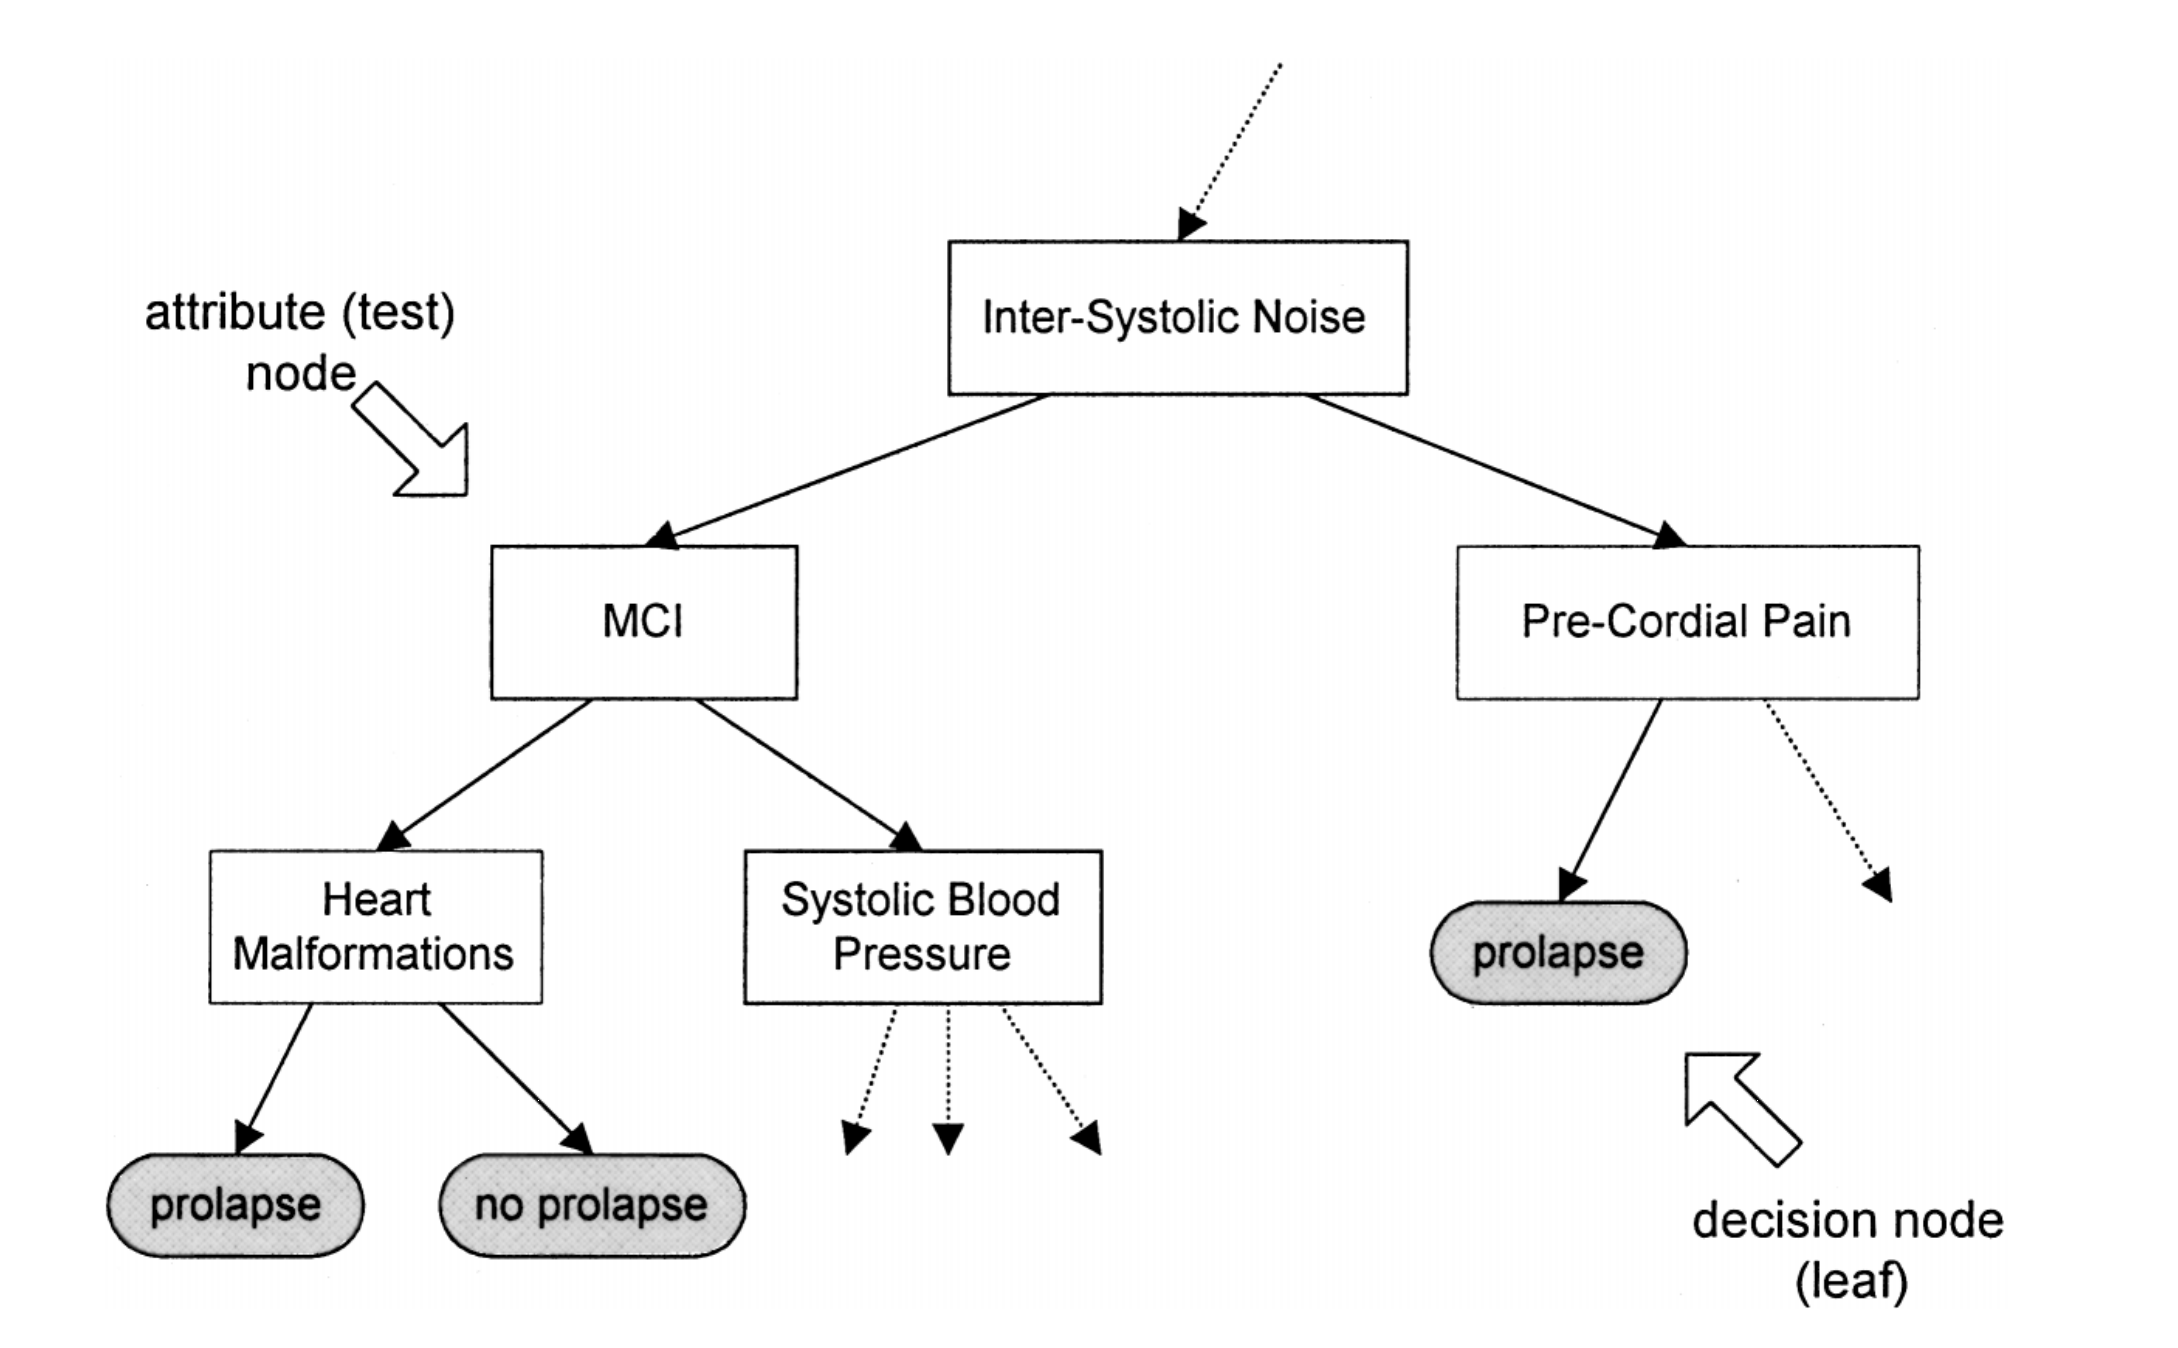
\includegraphics[scale=.4]{fig_decision_tree.png}}
    \label{fig:decision-tree}
    \legend{Source: ~\citet{Podgorelec2002}}
\end{figure}

%\subsection{Adaboost}\label{subsec:adaboost}
%
%\textit{Boosting} is an ensemble induction approach that achieves a similar effect to bagging, but without relying on randomness and the performance of each independently-induced classifier.
%Instead, boosting trains each new predictor based on the shortcomings of its predecessors, so they are correlated by an iterative improvement~\cite{Kubat2017}.
%Originally designed as the aggregate of three classifiers, boosting is adapted by the \textit{Adaboost} algorithm to have many more learners.
%The induction is done by the probabilistic selection of training examples in a way that reinforces ones with more misclassifications each time.
%Moreover, Adaboost uses \textit{weighted majority voting} with decision power (weights) concentrated according to performance~\cite{Kubat2017}.

%\textcolor{red}{\textbf{mention afterwards why not used}}

%\subsection{Support Vector Machines}\label{subsec:svms}
%
%Support Vector Machines (SVMs) are classifiers that find class separation boundaries for problems where there is "class overlap" in feature space (from which simple a linear boundary wouldn't make an accurate separation)~\cite{Hastie2009}.
%SVMs achieve this by transforming (enlarging) the feature space with non-linear \textit{kernel} function to enable higher-dimension hyperplane boundaries to separate the data.
%
%\textcolor{red}{\textbf{mention afterwards why not used}}

\subsection{Elastic Nets}\label{subsec:elastic_nets}

The Elastic Net (EN) is a regularization and feature selection method for linear or logistic regression that essentially combines two other regression methods called ridge and lasso.
It improves on lasso by generalizing it~\cite{Zou2005}.
The technique introduces a \textit{grouping effect} with which correlated variables stick together in regards to their relative contribution to the prediction, which can be estimated for the same usefulness as \textit{p}-values for assessing their importance~\cite{Burke2018}.
The nature of the algorithm begs the definition or selection of two hyperparameters: lambda (the regularization parameter) and alpha (the ridge-lasso-mixing parameter).

\subsection{Artificial Neural Networks}\label{subsec:anns}

Artificial Neural Networks (ANNs) are machine learning algorithms based on a graph structure of nodes (called \textit{neurons}) interconnected by weighted links.
Each neuron calculates an output that is a combination of its inputs (the network actual inputs or the outputs of other neurons) based on linear or non-linear functions.
Arranged in layers, these structures are also called \textit{multilayer perceptrons}, using \textit{forward propagation} to classify instances.
This process in the chain calculation of the neurons' activations up to the \textit{output layer}, where the prediction is decided to be class represented by the neuron with the highest value.
Based on a calculated error, the network updates its weights by the process called \textit{backpropagation}, implementing error minimization by \textit{gradient descent}~\cite{Kubat2017}.
Since ANNs are a large family of algorithms, many hyperparameters can be explored depending on the exact variation employed, but arguably the most basic ones are the number of hidden layers and neurons per in each hidden layer of the network.


\section{Ensemble Learning}\label{sec:ensemble-learning}

Supervised learning algorithms can be grouped to improve prediction performance and robustness, constituting an \textit{ensemble}.
This can be achieved by several different approaches, each with varying degrees of complexity.
The emerging trade-off between lesser interpretability by increased complexity and predictive power should always be considered, as its asymmetry is dependent on the domain, the dataset, and the underlying algorithms involved.
That said, it has been shown that, in general, good results can be achieved with relatively simple combinations of predictors~\cite{Clemen1989}.
Commonly employed techniques of lower complexity include:
\begin{itemize}
    \item majority voting: when the classification outcome is defined by the most predicted class among the ensemble's constituents;
    \item weighted averaging: when the class with the highest linearly-combined probability between constituents is chosen.
\end{itemize}

\subsection{Random Forests}\label{subsec:random_forests}

Random Forests are defined as ensembles of decision trees (grown considering random vectors) that classify instances by majority voting\cite{Breiman2001}.
Random forests are also useful for generating ranks of features importance by assessing the automatically computed variable importance measures (VIMs) of the forest~\cite{Boulesteix2012}.

This ensemble is trained using \textit{bagging}, an acronym for \textit{bootstrapping} and \textit{aggregation} (majority voting).
Bootstrapping works by composing a number of training subsets by sampling from the original training data with replacement, then inducing a tree classifier from each~\cite{Kubat2017}.
This process is illustrated in the left half of Figure~\ref{fig:random-forest}, while the right half shows how inference takes place.
Bagging performance depends on how well the classifiers perform for different examples (the dependence between classifiers), and the individual performance of each~\cite{Breiman2001}, coupled with the reliance that with sufficient randomness and forest size individuals' errors will be corrected by others~\cite{Kubat2017}.

\begin{figure}[H]
    \caption{A depiction of the random forest algorithm}
    \centerline{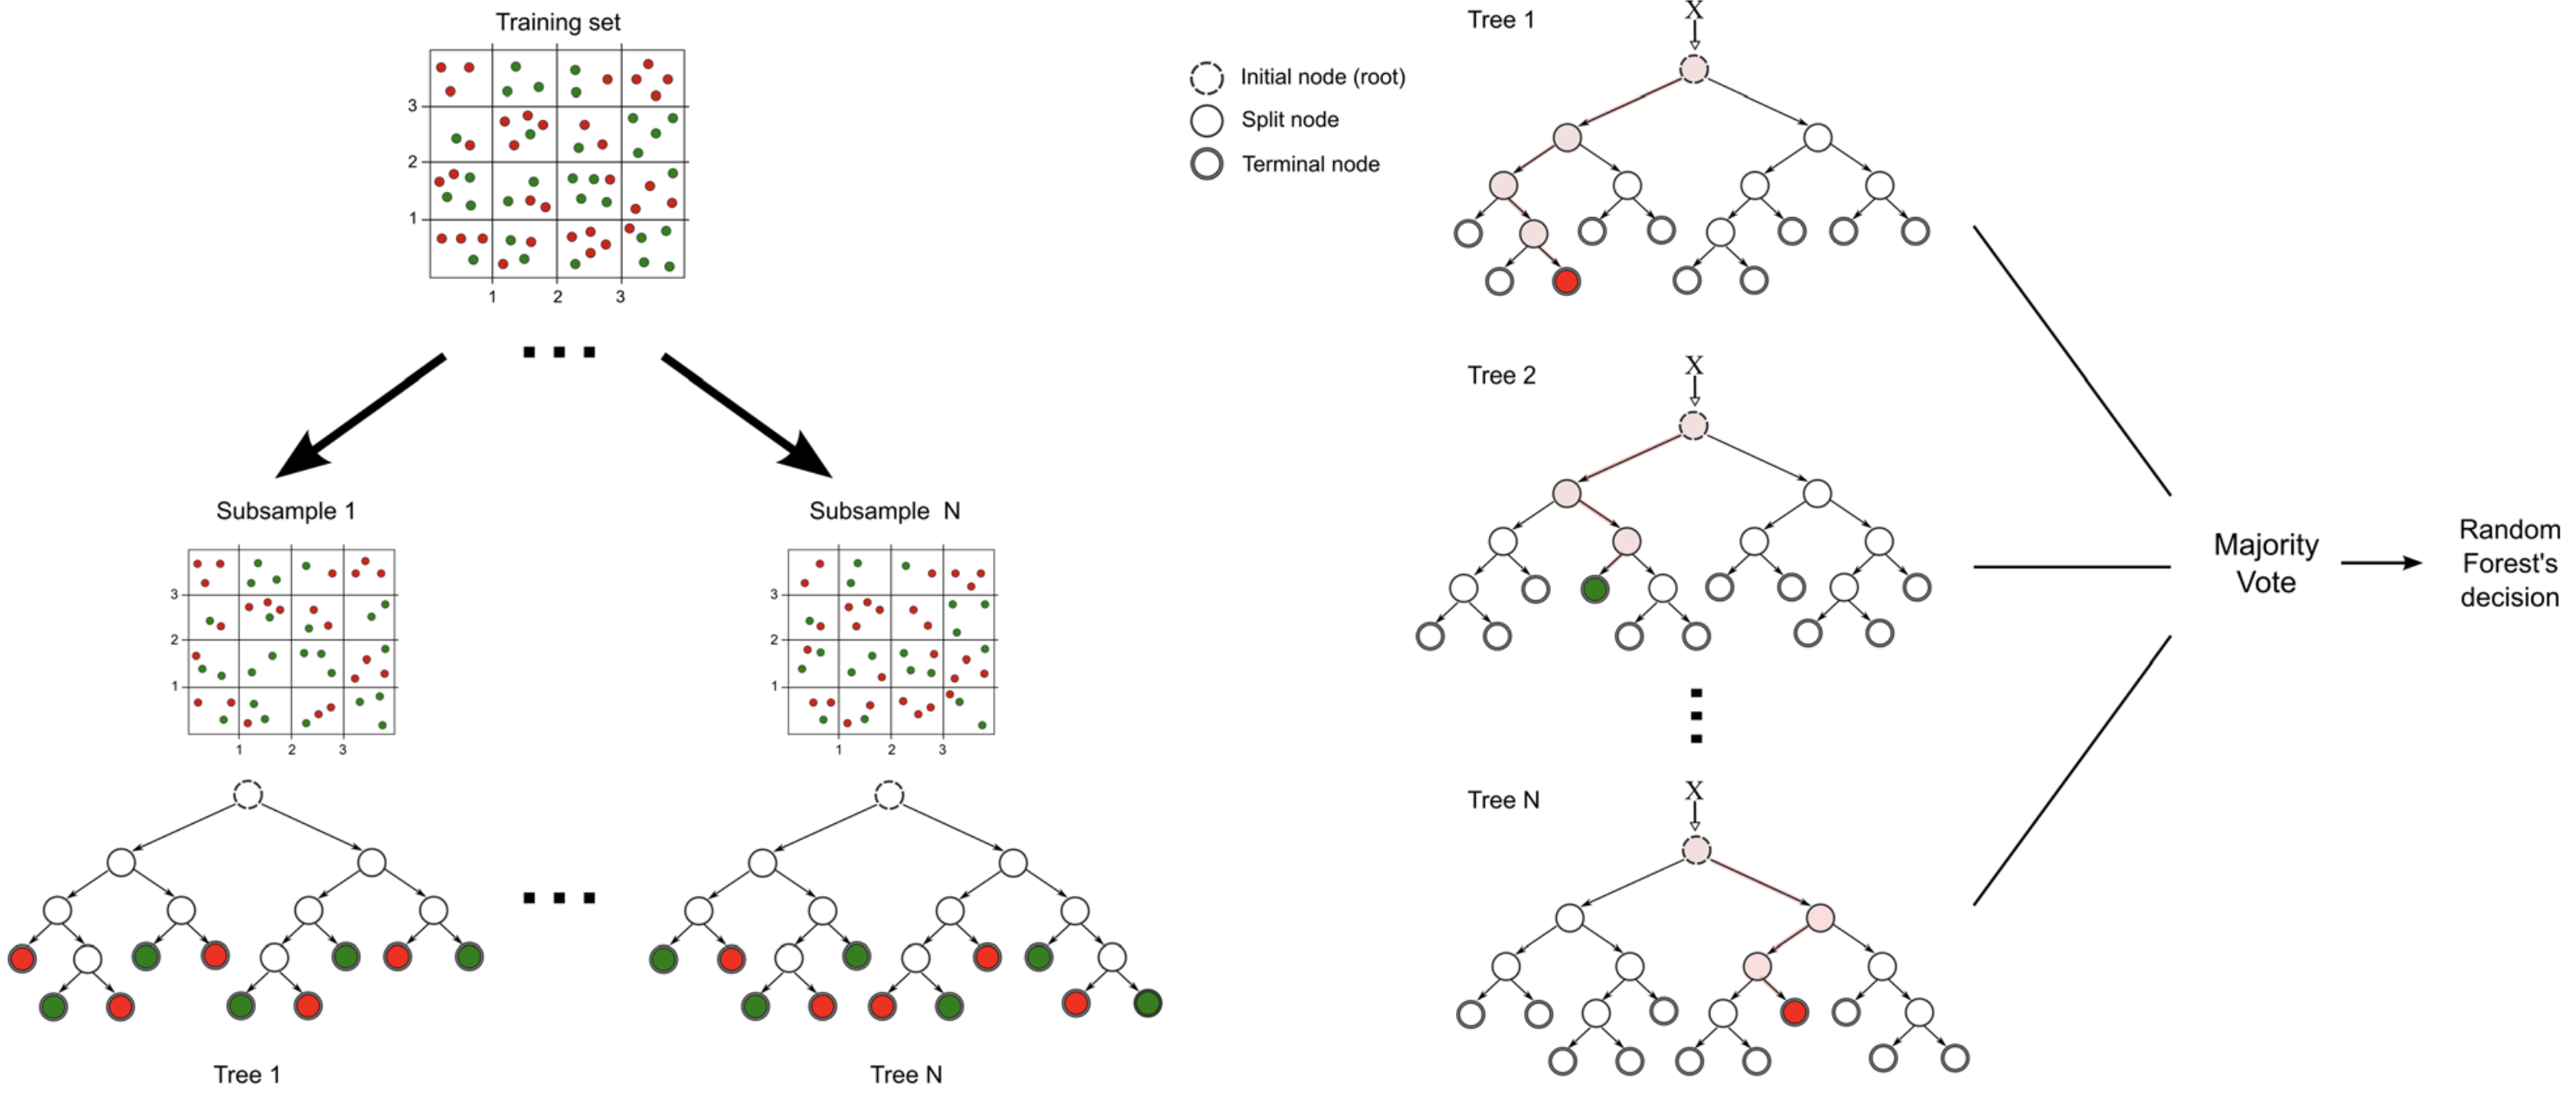
\includegraphics[scale=.27]{fig_random_forest.png}}
    \label{fig:random-forest}
    \legend{Source: ~\citet{Machado2011}}
\end{figure}

Injecting randomness in the procedure through \textit{random feature selection} in node splits can yield benefits in prediction performance including enhancement of generalization capacity and resilience to noise (variance), with overall results comparable to Adaboost (another tree-based ensemble algorithm, but based on boosting)~\cite{Breiman2001}.
Several variations on the classical random forests have been proposed, one of which being the Extremely Randomized Trees~\cite{Geurts2006}.
This algorithm differentiates itself from the others by its approach to node-splitting, which (as the name suggests) strongly randomizes the choice of attribute and cut-point.


\section{Feature Selection Wrappers}

Classification models can be improved upon, in regards to their interpretability and inference capability, by being embedded in a feature selection wrapper algorithm.
Different approaches to this optimization heuristic have been proposed, implemented, and tested.
A common and intuitive approach is Feature Elimination (FE), which has been shown to improve performance and reduce model complexity~\cite{Svetnik2004, Guyon2002}.
It consists of repeatedly eliminating irrelevant features to improve interpretability and performance upon model retraining.
The variable importances can be assessed once, the first time the model is trained, or reassessed each time the model is retrained, configuring a Recursive Feature Elimination (RFE)~\cite{Svetnik2004}.

%Evidence has been found that the learners wrapped RFE are more prone to overfitting \textcolor{red}{\textbf{Svetnik, V}} compared to ones wrapped in the non-recursive variant, although this evidence has been presented as being derived from "limited experience".


\section{Class Imbalance} \label{sec:class_imbalance}

The \textit{class imbalance problem} pervades machine learning research and applications in general~\cite{Chawla2009}.
A consequence of training from datasets skewed towards a majority class, it hinders the performance of classifiers by introducing biases in standard induction algorithms that work best with balanced distributions of classes~\cite{Japkowicz2000}.
This situation consistently manifests itself in medical diagnosis contexts~\cite{Vluymans2019a}, where it is common to have many more examples of some healthy (generally called \textit{negative}) class than the unhealthy (generally called \textit{positive}) one.
Moreover, the domains of application where these skewed distributions arise frequently have an inherently higher cost of mispredictions of the positive minority classes (e.g.\ labeling an ill instance as healthy)~\cite{Kotsiantis2013}.
Nevertheless, many works dealing with applications in mental health do not confer the appropriate attention to the evaluation and treatment of class imbalance~\cite{Burke2019}.
~\citet{Vluymans2019a} separates techniques for the mitigation of class-imbalance effects into four groups: data level preprocessing (\textit{external)}, algorithm-level (\textit{internal}) approaches, and cost-sensitive and ensemble learning.
The two latter are combinations or special applications of the two formers.
While data-level preprocessing consists of modifying the original dataset to have less class imbalance, algorithm-level approaches focus on slightly altering the mechanisms of standard learners to reduce their bias towards the majority class.

Data-level methods can operate by oversampling the minority class, undersampling the majority class, or combining the two.
Undersampling and oversampling can be done randomly or focused~\cite{Kubat1997, Laurikkala2001}, with reportedly mixed results of improvement of one over the other~\cite{Japkowicz2002}.
Oversampling methods work by copying or generating new instances.
In the latter category, the \textit{SMOTE} algorithm~\cite{Chawla2002} reportedly yields considerable performance gains from synthetically creating minority class examples.
In effect, it enlarges decision regions that contain nearby minority class points.

Cost-sensitive learning consists of enhancing the importance of minority classes by altering the amount of cost to different types of errors, classes, or features~\cite{Vluymans2019a}.
One example of this type of approach is MetaCost~\cite{Domingos1999}, which wraps general classifiers training with the introduction of a \textit{cost matrix} that assigns different costs to false positive and false negative errors.

Lastly, in a broad context, ensembles are usually employed for improving accuracy, which by itself would not be of much help for the class imbalance problem.
Thus, ensemble-based solutions for the class imbalance problem introduce specific adaptations, usually done by embedding data-level preprocessing methods or cost-sensitive learning in the induction of the ensemble~\cite{Vluymans2019a}.


\section{Model Evaluation} \label{sec:model-evaluation}

To correctly evaluate the performance of a classification model, it is necessary an understanding of some key concepts, briefly explained in this section.
Evaluation can be done with multiple techniques, assessing different metrics - each having peculiarities in relevance and interpretation depending on the specific context.
Deciding the correct metrics to employ is crucial when dealing with class-imbalanced data because not every metric adequately describes classification quality reliably in this scenario.

\subsection{Evaluation Metrics}\label{subsec:evaluation_metrics}

Since all performance metrics for classifiers correlate to the model's predictions of the labels (or classes) of instances (also called examples), it's useful to employ some common naming of the possible classification cases.
A binary classifier can either predict an instance's label correctly (inferring its true class) or incorrectly (inferring a false class).
When a positive class is inferred correctly, it's called a \textit{true positive}.
Conversely, a misprediction of a positive class is a \textit{false negative}.
The terms \textit{true negative} and \textit{false positive} have analogous definitions.
For convenience, throughout this paper, in the context of some set of predictions, we'll refer to the size of the subsets of \textit{true positives}, \textit{true negatives}, \textit{false positives}, and \textit{false negatives} as \textit{TP}, \textit{TN}, \textit{FP}, and \textit{FN}, respectively.

The first metrics that enable quantitative evaluation of a classifier are its accuracy and error rate.
Both concepts are very intuitive: accuracy is the rate of correct labeling of a set of predictions.
On the other hand, the error rate of this batch of inferences is the frequency of misclassifications.
Accuracy (\textit{Acc}) and error rate (\textit{E}) are therefore correlated (by $Acc = 1 - E$), and can be defined as follows~\cite{Kubat2017}:

\begin{equation}
    Acc = \frac{TP+TN}{TP+TN+FP+FN}
\end{equation}

\begin{equation}
    E = \frac{FP+FN}{TP+TN+FP+FN}
\end{equation}

However, error rate and accuracy are not good estimators for the performance of learners, especially in the presence of class imbalance.
It's easy to see why by imagining the following scenario.
Suppose some model learns from a dataset composed of 80\% negative-class instances (healthy dogs) and 20\% of positive-class instances (diseased dogs).
If measured by accuracy, this learner could be deemed quite successful by always predicting negative labels (asserting that all dogs it analyses are fine).
Yet, that predictor would be disastrous for identifying ill specimens, worse than useless - since animals bearing sickness would not be treated, after confidently being labeled healthy.
Thus, accuracy can mask a learner's problematic performance profile and misjudge its usefulness, especially with imbalanced datasets and false-positive-critical applications - a frequent case in clinical medicine~\cite{Vluymans2019a}.

Alternatively, we could evaluate classification capacity by measuring \textit{precision} (\textit{Pr}) and \textit{recall} (\textit{Re}).
These metrics improve on accuracy by focusing on a class of interest, providing better insight from \textit{TP}, \textit{TN}, \textit{FP}, and \textit{FN}~\cite{Kubat2017}.
Intuitively, precision is the probability that a learner is correct when inferring a positive class, whereas \textit{recall} measures if true positives are identified accordingly.
Depending on the context of the application, one would train its predictor with special attention to one of \textit{precision} or \textit{recall}.
Precision may be more desired in applications where we do not want our model to yield many false positives.
For example, in identifying criminals from pictures, we would not want to accuse innocents.
On the other hand, in studies of clinical conditions, \textit{recall} is generally the most important indicator, since we do not want to miss any positive instance by classifying it as a (false) negative.
We can see that minimizing false positives yields higher precision and minimizing false negatives yields higher recall by analyzing the formulas for these quantities:

\begin{equation}
    Pr = \frac{TP}{TP+FP}
\end{equation}

\begin{equation}
    Re = \frac{TP}{P} = \frac{TP}{TP+FN}
\end{equation}

When a learner changes its profile to be more prone to label instances as positive in general, it will probably increase \textit{recall} at the cost of reduced \textit{precision}.
Thus, a relevant performance metric is the F\textsubscript{\textbeta }-Score, which combines precision and recall in a weighted harmonic mean.
The \textbeta{} factor defines which of the two quantities will have more importance in the measure.
The F\textsubscript{2}-Score is particularly interesting in clinical applications where positive instances are fewer in number and at the same time more important to be noticed (i.e. FNs are more costly).
This is because this metric is affected by changes in the class distribution~\cite{Tharwat2018}, and has an intuitive meaning of its user valuing recall two times more than precision~\cite{C.J.vanRijsbergen1977}.
The F\textsubscript{2}-Score can be reduced to the following equations:

\begin{equation}
    F_2 = \frac{5*TP}{5*TP+4*FN+FP}
\end{equation}

\begin{equation}
    F_2 = \frac{5*Pr*Re}{4*Pr+Re}
\end{equation}

Other important metrics for the medical domain are \textit{sensitivity} and \textit{specificity}.
Although quite traditional to the field, these indicators are rarer in machine learning studies in general~\cite{Kubat2017}.
\textit{Sensitivity} is another name for \textit{recall}, while \textit{specificity} is essentially \textit{recall} for the negative class.
More precisely:

\begin{equation}
    Se = \frac{TP}{P} = \frac{TP}{TP+FN}
\end{equation}

\begin{equation}
    Sp = \frac{TN}{N} = \frac{TN}{TN+FP}
\end{equation}

Just as there is often a trade-off between precision and recall, sensitivity and specificity can vary at odds with each other.
This inference-behavior changes, reflecting the balance between sensitivity and specificity under different hyperparameters, are illustrated by \textit{receiver operating characteristic} (ROC) curves~\cite{Kubat2017}.
These graphs portray sensitivity (also called \textit{true positive rate}) on the y-axis versus a proxy for specificity named \textit{false positive rate} (also called \textit{false alarm rate}) on the x-axis.
The \textit{false positive rate} is defined as~\cite{Fawcett2006}:

\begin{equation}
    Fpr = 1 - Sp = \frac{FP}{N} = \frac{FP}{TN+FP}
\end{equation}

ROC space has some notable points, each translating to a characteristic behavior in classification profile~\cite{Fawcett2006}:
\begin{itemize}
    \item (0,0): to always infer the negative class
    \item (1,1): to always infer the positive class
    \item (0,1): to always infer the correct class
\end{itemize}

%For a given ROC curve, we can identify optimal classifiers by considering only the ROC \textit{convex-hull} (ROCCH), instead of all the available points~\cite{Fawcett2006}.
%These points in the ROC space represent, intuitively, classifiers with lower expected cost, positioned in the northwestern extremities of the graph.
%A classifier is optimal if and only if it lies in the ROCCH~\cite{Fawcett2006}, so we can discard the sub-optimal models and consider only the ones over the convex-hull.
%This graph section is also useful for class imbalance performance assessment.
%Because of the ROC graphs invariance to class imbalance or error costs, one can derive \textit{iso-performance lines}~\cite{Provost2001} and find optimal classifiers over a specific range of the hull for defined class skews and costs.

Based on the analysis of ROC curves, it is customary to consider a classifier's \textit{area under the ROC curve} (\textit{AUC} or \textit{AUCROC}) - a scalar value~\cite{Fawcett2006}.
A perfect classifier will have \textit{AUC}=1, since its ROC curve will be the point (0,1).
The area under the ROC curve can be interpreted as a model's capacity to distinguish instances of different classes as so - it may also be interpreted as the probability of ranking a positive random instance higher than a random negative one~\cite{Fawcett2006}.
It is important to note, however, that the AUCROC is also subject to hiding the true performance of a model under class imbalance, although not as much as accuracy.
With imbalanced classes, a high AUC could merely indicate a better capacity for identifying negative instances~\cite{Burke2019}.

In conclusion, as each approach has its strengths and weaknesses, it is prudent to consider multiple metrics assessments to have a holistic evaluation of classification models.

\subsection{Evaluation Methodologies}\label{subsec:evaluation_methodologies}

With the interest of inducing the best classifier in our reach, we are now ready to consider the methods for using performance metrics to achieve our goal of evaluating and choosing machine learning models.
Several algorithms could be leveraged for that - hence we'll discuss baseline approaches, \textit{random subsampling}, \textit{N-fold Cross-Validation} (CV), and \textit{stratification}.
Nevertheless, The general idea is to perform a \textit{model selection}, choosing the one with parameters that yield the best results, or to perform a final evaluation purely for estimation of performance on unseen data.

The ideal approach for model selection and evaluation would be to separate our dataset into three parts - for training, validation, and tests~\cite{Hastie2009}.
The validation set would be used to assess the performance of models trained with the training set, while testing instances would be reserved for evaluating the chosen best classifier.
There is also the approach to separate the data into only two sets (training and testing)~\cite{Kubat2017}.
Although this could lead to test-error underestimation, this is done to check the generality of the learner~\cite{Hastie2009} - or else we could deem desirable a model overfit to the training data, with no guarantees of extending its prediction capability to new instances.
Both methods are suitable for situations with data abundance.
With smaller datasets, the distribution of instances within each subset is subject to be substantially different from the original dataset~\cite{Kubat2017} - especially with class-imbalanced data.

As an alternative to these standard approaches, one could use \textit{random subsampling} to mitigate the limitations in distribution representation fidelity of the subsets of the baseline methods.
The difference in this procedure is that the training and testing separation is repeated multiple times, each composing different subsets randomly~\cite{Kubat2017}.
This yields, each time, some performance metrics, which are averaged to finish the evaluation.

On the other hand, instead of randomly repeating the training-testing division, the dataset could be divided into K equally-sized parts (also called \textit{folds}, typically 5 or 10).
Then, for each fold, have a round of training, evaluations, and improvements, using the fold as a validation set and the others for training~\cite{Hastie2009}.
One key (advantageous) difference that arises from this approach, called \textit{K-fold cross-validation}, compared to \textit{random subsampling}, is that each of the training sets (and test sets) is disjoint from the others~\cite{Kubat2017}.
This concept can be extended to incorporate a repetition (then being loosely named N-times K-fold cross-validation), where new cutting-points to separate the folds are selected each time, to achieve assessments with more statistical robustness.

Although promising, CV is subject to problems when dealing with highly imbalanced datasets;
the distribution of instances within folds could bear little resemblance to the complete dataset~\cite{Kubat2017}. \textit{Stratified} approaches mitigate this by guaranteeing that all the folds have the same class ratio, respecting the original data's distribution.


    \chapter{Related Work} \label{ch:related_work}
    To better understand the scenario of machine learning studies in medicine in recent years, and specifically in the field of mental health, a systematic literature review (SLR) was brought to analysis.
~\citet{Burke2019} focused its attention on suicide-related applications and employed a methodology oriented by inclusion and exclusion criteria, where papers from multiple sources were processed through a systematic pipeline.

The SLR targeted papers published until February 2018 in the PsycINFO, PsycARTICLES, ERIC, CINAHL and MEDLIN databases.
From an initial set of 288 retrieved studies, derived by search terms of methodological (e.g.\ "machine learning", "data mining" and "big data") and domain ("suicide", "self-injury", "suicide ideation") imprint, only 35 papers met the inclusion criteria and went on to further analysis.

As for the conclusions of the review, we are interested mainly in its insights on the successes and difficulties of previously employed ML algorithms in problems with similar characteristics to ours - to predict suicide ideation.
The study was able to demonstrate the potential of ML algorithms in the mental health field;
it was shown that this branch of technology can greatly improve the prediction performance of mental disorders.
Furthermore, the exploration and finding of predictor variables replicate established results but also find novel variables and identifies subgroups of interest.
This SLR also emphasizes the importance of the interpretability of the models and their trade-off over performance.
To that extent, this subset of the literature tends to favor simpler predictors like decision trees.
As \autoref{fig:burke-algorithm-prevalence} shows, over 60\% of the analysed papers employed DTs, while ANNs (a generally less interpretable model, though a strong performer in a myriad of applications) appeared only in about 10\% of the articles.

\citet{Burke2019} separate the study of suicide into distinct (though sometimes intersecting) categories: suicide death, suicide attempt, suicide planning, and suicide ideation.
SI studies (a small subset of only 10 papers in this SLR) used both cross-sectional and longitudinal designs (with one to five years follow-ups), considering data from population samples distinct in age, locale, and mental health.
The trained models incorporated, on average, 32 attributes (ranging from 3 to 62), and each study used one to four (M=1.6) ML methods.
Almost all of the ten papers used structure data, safe from one that employed an NLP approach.
As for the performance metrics, however, the inconsistency in strict and standardized reporting is evident.
Some papers do not show any performance estimation whatsoever, while others generally do not share the same indicators and scores (reporting exclusively AUC-ROC, accuracy, or sensitivity and specificity, etc.).
Along with the small paper sample size, this makes the effort to derive statistics on their models' performance futile.

Nevertheless, the reported metrics are indicative of the potential of employing the algorithms from \autoref{fig:burke-algorithm-prevalence} in the prediction of suicide ideation.
As~\citet{Burke2019} compiled, suicide ideation prediction studies reported AUC values ranging from 0.8 with DTs~\cite{Handley2014} to 0.92 with DTs and RFs~\cite{Gradus2017}, and sensitivity and specificity reaching 0.88 and 0.94~\cite{Just2017} with decision trees, neural networks and Support Vector Machines (SVMs), although considering only 34 data points, half of which were of the positive class).

Besides the gaps and inconsistencies in reported performance, Burke's SLR brings to light the lack of consistency and depth in treatment and discussions of class imbalance in training data in the analysed studies.
While many papers report AUC, which better describes the performance than just the accuracy, it still falls short in completely describing the actual performance of the predictor in the presence of class imbalance~\cite{Burke2019}.
And while some papers report precision and recall, few studies address the problem of unbalanced data in their sampling and training.

\begin{figure}[h]
    \caption{Algorithms prevalence from~\citet{Burke2019}}
    \centerline{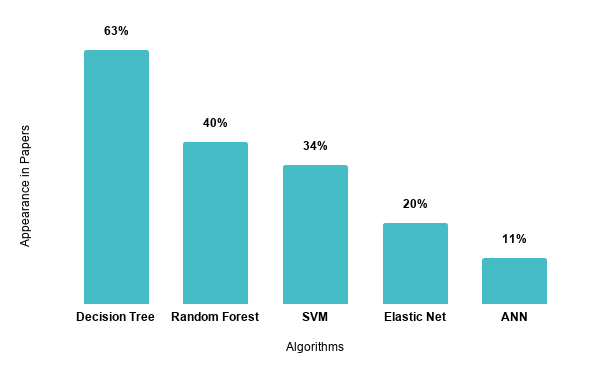
\includegraphics[scale=.75]{fig_burke_alg_usage.png}}
    \label{fig:burke-algorithm-prevalence}
    \legend{Source: Author}
\end{figure}

That said, even though the beneficial attribute selection (for data dimensionality reduction) and class-imbalance mitigation techniques are oftentimes lacking in classifications problems in the context of mental health ~\cite{Burke2019}, that is not always the case.
An example of successful attribute selection is presented in ~\cite{Barros2017}, which used a wrapper-based method in a Chilean mental-health patients dataset to reduce the feature set size from 343 to 22, reporting sensibility and specificity between 0.7 and 0.8, approximately.
On the other hand, in the context of class-imbalance reduction, ~\citet{Schubach2017}} employs both downsampling of the negative class and oversampling of the positive class (with the SMOTE algorithm) to balance data partitions and train a random forest on each, afterward combining them in what is described as an ensemble of ensembles.
The models' performance estimation from~\citet{Schubach2017} varied substantially depending on the evaluated dataset, achieving at best around 0.7 area under a precision and recall curve, but at worst barely over 0.4.
That said, the calculated AUCROC was always around 0.98 (again showing a problem in relying only on this metric).

Since the afore-mentioned SLR did not review works after February 2018~\cite{Burke2019}, it is also worth mentioning some related works developed since then - again, searching for insights on their achievements and limitations, bringing to light their similarities to our study.

With a similar problem to the one our work aims to solve, future risk of suicidal thoughts was chosen as the outcome variable to the models of ~\citet{Roy2020}, although the employed data was unstructured (text, from Tweeter).
The study considered a vast amount of tweets per individual, but on the other hand, the suicide ideation cases in the dataset were less than 300.
That said, the study achieved a high AUCROC value of 0.88 using a model that combines the outputs of several neural networks using a random forest.

Using structured data from Korean population samples, two studies~\cite{Oh2020, Jung2019} also tackled problems akin to ours, with similar approaches too.
Both proposed to solve the problem of classification of suicide ideation (with our without suicide attempt), but with different datasets.
The first focused adults~\cite{Oh2020} and the second on adolescents~\cite{Jung2019}.
With over 16,400 instances, the Korea National Health and Nutritional Examination Survey (KNHNES) data employed in~\citet{Oh2020} is more than four times larger in this regard than our restricted (to common mental disorders) sample of the ELSA-Brasil dataset.
On the other hand, although the Korean Young Risk Behavior Web-basedSurvey (KYRBWS) dataset from~\citet{Jung2019} included data from over 62,200 adolescents, ~\citet{Jung2019} employed a drastic downsampling strategy in its preprocessing, achieving class balance to the cost of reducing the instances count to approximately 15,300 - just as the data in ~\citet{Oh2020}, amounting to approximately 400\% of our dataset size.

As far as assessed variables are concerned, a key difference between a fully automatic approach to variable selection (as we propose in Chapter~\ref{ch:methodology}) and the one from~\citet{Oh2020} is that the study resorted to filtering based on the manual inspection and review of two health professionals, reducing the dimensionality from 800 variables to only 48.
That said, ~\citet{Oh2020} also employed wrapper-based feature selection in their computational methodology, in a similar way to our efforts in that regard.

In regards to classification qualities, the best model from~\citet{Jung2019}, an artificial neural network, was estimated to have an AUCROC of almost 0.88, with sensibility of around 0.81 and specificity close to 0.77.
The most successful algorithm used in ~\citet{Jung2019} (called \textit{extreme gradient boosting}) yielded very similar results, with slightly lower AUCROC and sensitivity and higher specificity.
Since these two studies also report the estimated positive predictive values (precision) of their classifiers, we can also calculate their F\textsubscript{2}-Scores, which amount to 0.48~\cite{Oh2020} and a distinguishing value of 0.84~\cite{Jung2019}.

Finally, in Brazil, some studies have already employed machine learning techniques over the ELSA-Brasil dataset.
Both~\citet{Brunoni2020} and~\citet{Librenza-Garcia2020} treat as dependant variables the depression incidence or persistence - in other words, how interviewees' depression evolves in the four years between the two ELSA-Brasil waves.
While~\citet{Brunoni2020} focused on analyzing the risk factors of depression, ~\citet{Librenza-Garcia2020} performed a similar classification task to our own, with an elastic net reportedly having sensitivity of 0.67, specificity of 0.78, and AUCROC of 0.79.
Since ~\citet{Librenza-Garcia2020} also reported the precision of its model, we can estimate its F\textsubscript{2}-Score as 0.45.

A summary of the performance of some of the studies mentioned in this chapter is presented in Table~\ref{tab:related-work-comparison}, which has empty cells for the metrics that were not reported and could not be derived.
The works included in the table are the ones that presented the most similarities to ours in scope and approach and are ordered by the F\textsubscript{2}-Score and the AUCROC\@.
Although the best performance is attributed to an application of the eXtreme gRadient Boosting (XGB) algorithm~\cite{Jung2019}, it is worth noting that this is not necessarily the most decisive factor to its success: the study employed the largest dataset between the ones presented in the table by a substantial margin, and was able to circumvent the class-imbalance problem by discarding a huge chunk of the data and yet remain with a high number of instances.

\begin{table}[h]
\caption{Summary of performance estimates of related works}
\begin{center}
\begin{tabular}{c|c|c|c|c|c}
\textit{Paper} & \textit{Algorithm} & \textit{F\textsubscript{2}-Score} & \textit{AUCROC} & \textit{Sensitivity} & \textit{Specificity} \\
\hline
\hline
A              & XGB                & 0.84              & 0.86            & 0.79                 & 0.79                 \\
B              & ANNs + RF          & 0.71              & 0.88            & 0.80                 & 0.79                 \\
C              & ANN                & 0.48              & 0.88            & 0.81                 & 0.77                 \\
D              & EN                 & 0.45              & 0.79            & 0.67                 & 0.78                 \\
E              & RFs                &                   & 0.98            &                      &                      \\
F              & RF                 &                   & 0.92            &                      &                      \\
G              & SVM                &                   &                 & 0.77                 & 0.79                 \\
\hline
\end{tabular}
\end{center}
\legend{Source: The Author

A: ~\cite{Jung2019};

B: ~\cite{Roy2020};

C: ~\cite{Oh2020};

D: ~\cite{Librenza-Garcia2020};

E: ~\cite{Schubach2017};

F: ~\cite{Gradus2017};

G: ~\cite{Barros2017}.}
\label{tab:related-work-comparison}
\end{table}


    \chapter{Methodology}\label{ch:methodology}
    This chapter describes our methodology to approach the problem of prediction of suicidality using machine learning algorithms.
First, we present the dataset used (the ELSA-Brasil study) and the steps adopted during its cleansing.
Next, we describe our model-induction pipeline for a set of supervised learning algorithms of interest.
Finally, we explain our strategies for model evaluation and for building an ensemble classifier.

Our proposal to approach the problem of prediction of suicidality can be summarized in three steps.
First, the data (in our case, from the \textit{ELSA-Brasil} study) is cleansed and minimally prepared.
Afterward, it is used by a model-induction pipeline, for a set of supervised learning algorithms of interest.
Finally, the models are evaluated and combined in an ensemble (which is also evaluated in the same manner).


\section{Dataset}\label{sec:dataset}

The Brazilian Longitudinal Study of Adult Health (ELSA-Brasil) dataset is a cohort of Brazilian adults (public universities' employees) in a longitudinal study with a follow-up of about 4 years~\cite{Schmidt2015, Aquino2012}.
Up to now, two waves of interviews and examinations have been conducted: the first from 2008 to 2010, the second from 2012 to 2014~\cite{Olivera2017}.
The baseline assessment included 15105 participants, with about 3000 assessed variables (although the availability of the attributes is restricted depending on the application).
Given the scope and context of our application, after requesting data access with the interest of investigating suicidality, a version of the ELSA-Brasil dataset was made available to this study that includes 2288 "baseline" features.

Moreover, the ELSA-Brasil study assessed non-psychotic psychiatric morbidity using the Clinical Interview Schedule-Revised (CIS-R) ~\cite{Nunes2016, Lewis1992}, which makes available information regarding depressive and/or suicidal thoughts on the cohort.
The full version of the applied CIS-R questionnaire is made available in annex ~\ref{ch:cis-r}.
Although the full array of 176 questions is not explored in this section, the ones found to be of most importance are discussed in Chapter~\ref{ch:experiments-and-results}.

In our work, we analysed only the first wave of the study and focused on a specific population of the ELSA-Brasil dataset, corresponding to the individuals presenting any common mental disorders, indicated by the \textit{mentalvar\_A\_TMC} feature.
The reason for restricting the dataset is that our goal is not to develop a model that identifies the presence of suicidality in the general population, as this would have limited utility, but rather to identify this condition for a population at risk.
Individuals with CMD are probably under the assistance of mental health professionals, who could act upon the suggestion of machine learning classifiers that the patient is prone to suicidal ideation and, by proxy, suicide attempts.
Besides, we also avoid broadening too much the training dataset to the point where class imbalance becomes too severe to handle, as the prevalence of suicidality is about 8.53\% in this cohort.
Although there is a clear trade-off between the ratio of instances in the positive class and the total number of instances in the training data, we apply this restriction since in our domain it is indispensable to make correct predictions for the positive class.
As a result of excluding the instances without CMD, our number of data points is reduced from 15105 to 4039, incurring the loss of 169 (13.11\%) positive class instances, but raising the probability of the class from 8.53\% to 27.73\%.

\subsection{Input Variables - Features}\label{subsec:features}

Besides socio-demographic and economic attributes, the ELSA-Brasil study assessed the participants' health in different aspects and means, from electrocardiograms to retinal photographs and mental health questionnaires~\cite{Schmidt2015}.
The available data in ELSA-Brasil includes attributes previously described in the literature as associated with suicide ideation, including gender, age, marital status~\cite{Nock2008}, socioeconomic status~\cite{Gunnell2009, Meltzer2012, Meneghel2004}, physical activity, alcohol consumption, self and family education levels~\cite{Souza2010a} and emotional difficulties (e.g.\ deaths of close relatives), social capital variables, pain conditions, chronic diseases, obesity and body mass index, the existence of physical disabilities~\cite{Meltzer2012a}, and sexual orientation~\cite{Silenzio2007}.

As predictors of our models, we used all 2288 variables from the baseline dataset.
Besides, we also included variables from the CIS-R questionnaire, which, after excluding the variables used as outcomes, consists of 173 variables.
Therefore, the total number of predictors before data cleansing was 2461 features.

\subsection{Outcome Variables - Labels}\label{subsec:labels}

To represent the concept of suicidality, which is the outcome of our classifiers (i.e.\ a binary factor indicating the presence or absence of suicidality for a given instance), we assess and combine hopelessness, "taedium vitae", and suicidal ideation in logical disjunction, a boolean \textit{OR}.
These variables are, respectively, indicated by the responses to the CIS-R's H6, H8, and H9 questions:
\begin{itemize}
    \item CIS-R H6 (hopelessness): \textit{Have you felt hopeless at all during the past seven days, for instance about your future?}
    \item CIS-R H8 (taedium vitae): \textit{In the past week have you felt that life isn't worth living?}
    \item CIS-R H9 (suicidal ideation): \textit{In the past week, have you thought of killing yourself?}
\end{itemize}

Although the formulation of the questions implies a naturally binary "yes or no" response, both H8 and H9 have a third option, which is of presenting taedium vitae or suicidal ideation but not exactly in the last 7 days.
To this study, the third-option responses are considered as positive ones (i.e., as if the person had responded to the questions with a "yes").
These variables had several missing values since the majority of the interviewees did not reach the point of being asked their respective questions - they responded negatively to prior ones that are more general, such that we can assume there is an implicit negative answer to the more specific ones which we are interested.
Thus, absent values for CIS-R's H6, H8, and H9 variables were inferred as negative entries.

\subsection{Data Cleansing}\label{subsec:cleansing}

As a stride in the direction of improving data quality for the induction of the models, it is desirable to validate and clean (or \textit{wrangle}) the data before usage.
~\citet{Kandel2011} describe data wrangling and analysis as an iterative process consisting of cleansing, merging, adapting, and evaluating the data.

Considering that the ELSA-Brasil study has several variables obtained by non-linear interviews (skipping questions depending on answers), some instances present missing values.
Although our methodology includes a mechanism for inference of unavailable (NA) values (see Section ~\ref{sec:preproc-train-eval}), we considered important for data fidelity and for model quality to leave aside variables that have more NAs than a certain threshold - which we set as 10\% in this study.

Our solution does not include any natural language processing techniques, thus all free-text variables in ELSA-Brasil were removed.
We provide a list of textual variables removed in Table~\ref{tab:free-text-removed}.

Finally, and perhaps most importantly, given the chosen CIS-R questions (H6, H8, and H9) to be combined into our outcome label, we removed the predictors that indirectly make use of these variables - except for \textit{mentalvar\_A\_ESCORETOTAL}, which is adapted to be the sum of the numerical value of answers in the CIS-R H section excluding H6, H8, and H9.
These are, in the dataset, the variables shown in Table~\ref{tab:removed-info-leak}.
This step is crucial to avoid data leakage in model training, where our input variables (i.e.\ predictors) would improperly contain information about the outcome to be predicted.

\begin{table}[h]
    \caption{Attributes removed for introducing information leakage}
    \begin{center}
        \begin{tabular}{l|l}
            \textit{Attribute}           & \textit{Description}                     \\
            \hline
            \hline
            mentalvar\_\_TMAD            & Mixed anxiety-depressive disorder (MADD) \\
            mentalvar\_a\_DEP            & Major depressive disorder (MDD)          \\
            mentalvar\_A\_DEPGRAVE       & Severe MDD                               \\
            mentalvar\_A\_DEPLEVCSINT    & Mild MDD with somatic symptoms           \\
            mentalvar\_A\_DEPLEVSSINT    & Mild MDD no somatic symptoms             \\
            mentalvar\_A\_DEPMODCSINT    & Moderate MDD with somatic                \\
            mentalvar\_A\_DEPMODSSINT    & Moderate MDD no somatic                  \\
            mentalvar\_A\_ESCORETOTAL    & CMD score (continuous)                   \\
            mentalvar\_A\_SINTIDEIADEP   & Depressive thoughts symptoms             \\
            mentalvar\_A\_TMC            & Common Mental Disorder (CMD) (bin)       \\
            mentalvar\_A\_TMCGRAV        & Common Mental Disorders (CMD) (3 levels) \\
            mentalvar\_MDD\_trajectories & group(a\_DEP b\_DEP)                     \\
            mentalvar\_only\_incident    & Incident MDD                             \\
            mentalvar\_only\_remitted    & Remitted MDD                             \\
            \hline
        \end{tabular}
    \end{center}
    \legend{Source: The Author}
    \label{tab:removed-info-leak}
\end{table}

Upon removal of these variables, it is desirable to supply the models with some sensible substitute to the data that was taken away, since the variables were of great importance for the clinical diagnosis of suicidality.
Since interpretations of responses to the H section of CIS-R were summarized in the removed features, the idea is that the learners would instead interpret these relations by themselves given the necessary data.
Thus, our cleansing needs steps to also impute missing values in CIS-R answers, which were frequent given the interview is non-linear, so they are not removed by our afore-mentioned 10\%-maximum NA filter.
For this task, we realized that the majority of the answers could be reliably inferred from the context, if the person responded negatively to a question X, then some question Y which only makes sense if X was answered positively can be inferred to be negative too.

In conclusion, because of absent values, textual input, and information leakage, our cleansing procedure reduces the number of predictors to be employed in the model-fitting process, represented in Table~\ref{tab:dataset-cleansing}, and does not change the number of instances in the data.
The final high-level quantitative characteristics of our dataset are summarized in Table~\ref{tab:final-dataset-characteristics}.

\begin{table}[h]
    \caption{Number of variables in light of dataset cleansing process}
    \begin{center}
        \begin{tabular}{c|c}
            \textit{Attribute Set}        & \textit{Set Size}       \\
            \hline
            \hline
            Total (uncleansed)            & 2463 (100\%)            \\
            Removed (information leakage) & 13 (0.69\%)             \\
            Removed (NA excess)           & 773 (31.38\%)           \\
            Removed (free-text)           & 47 (1.91\%)             \\
            \textbf{Remaining (cleansed)} & \textbf{1626 (66.02\%)} \\
            \hline
        \end{tabular}
    \end{center}
    \legend{Source: The Author}
    \label{tab:dataset-cleansing}
\end{table}

\begin{table}[h]
    \caption{Main quantitative characteristics of cleansed dataset}
    \begin{center}
        \begin{tabular}{c|c}
            \textit{Dataset Characteristic} & \textit{Value} \\
            \hline
            \hline
            \#Instances                     & 4039           \\
            \#Attributes                    & 1626           \\
            \#Positives                     & 1120 (27.73\%) \\
            \#Negatives                     & 2919 (72.27\%) \\
            \hline
        \end{tabular}
    \end{center}
    \legend{Source: The Author}
    \label{tab:final-dataset-characteristics}
\end{table}


\section{Pre-processing, Training, and Evaluation}\label{sec:preproc-train-eval}

The goals in the proposed approach to produce our learners are: to attain interpretability and prediction performance.

With this goal in mind, we define our methodology considering the particularities of our dataset that make the development of predictive models particularly challenging.
The adopted dataset is highly skewed towards a majority class of non-suicidal instances, such that our procedures require the usage of techniques to mitigate class imbalance biases and to appropriately evaluate model performance in such a scenario.
There is also the problem of having numerous features for each instance, which can make it harder for the learners to have both good predictive qualities and interpretability.

\subsection{Pipeline and Pre-Processing}\label{subsec:pipeline-and-preprocessing}

The ordered combination of the main steps of our approach is summarized in the three-staged pipeline diagram of Figure~\ref{fig:train-pipeline}.
The highest layer, of evaluation, encompasses the whole cleansed dataset and orchestrates the fitting of models (abstracted by lower layers) and their performance assessment for each supervised learning algorithm.
The RFE procedure has its own layer (in blue), where the data is each training fold of the evaluation phase (also in blue), so the final test data is never used in induction.
Finally, within the scope of the yellow data boxes, the RFE models training folds, the most basic supervised learning layer (also in yellow) induces classifiers with hyperparameter tuning.

To avoid data leakage in the base learners induction, pre-processing is only applied in the lowest layer of our pipeline.
If pre-processing were applied before, the training data in the lowest layer would have been processed in a manner that uses information from its corresponding test data.
In this undesirable scenario, we could expect to have models with optimistic performance estimates that would perform (drastically) differently upon inferences on new data.

\begin{figure}[]
    \caption{Preprocessing, training and evaluation pipeline}
    \centerline{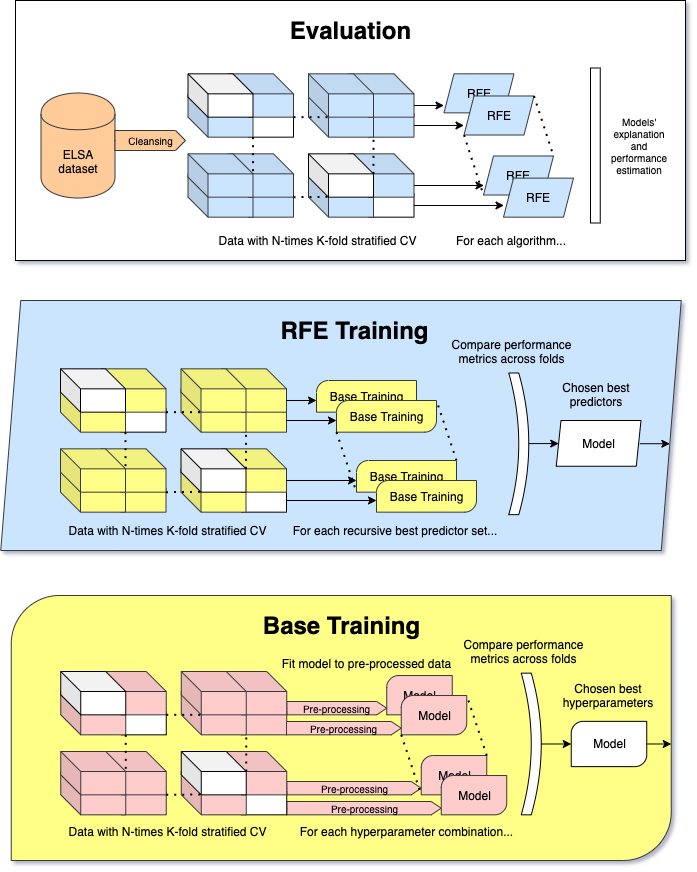
\includegraphics[scale=.6]{fig_pipeline_diagram}}
    \label{fig:train-pipeline}
    \legend{Source: Author}
\end{figure}

The preprocessing itself is proposed to be a sequential application of the following steps, each parameterized and described as general procedures:
\begin{itemize}
    \item \textbf{downsampling}, removing negative instances until the class distribution is of a given ratio (e.g.,\ 2N:1P, 3N:2P, etc - but not 1:1);
    \item \textbf{NA imputation}, inferring missing values using a function of the respective predictor values (e.g.\, the mean, or some classification or clustering ML technique, etc.);
    \item \textbf{near-zero variance (NZV) cut}, excluding useless predictors with a uniformity of values, defined by a parameterized quantitative criteria (e.g\, frequency distribution thresholds);
    \item \textbf{high-correlation filtering}, removing variables that are highly correlated to others (i.e.\ with correlation over a threshold) and that do not present distinct and useful information;
    \item \textbf{SMOTE}, synthetically creating positive instances derived from a fixed number of nearest neighbors (e.g.\ 3, 5, 7 etc) until the class distribution is of a given ratio (e.g.\ 1:1), (nearly) balancing the ratio of observations per class.
\end{itemize}

Note that the pre-processing steps of the pipeline do not necessarily promote perfect class balance for subsequent model induction.
This is controlled by adjusting the parameters related to the balance ratio, taking into account whether the supervised learning algorithm by itself can deal with the class imbalance to some extent.

\subsection{Model Induction Approach}\label{subsec:model-induction-approach}

We also aim to reduce the number of attributes of the data used in training and predictions to have a more interpretable classifier, from which clinicians can obtain intuitive knowledge.
In our work, we applied RFE to wrap "base learners" in a feature selection loop, where a model will have as the final predictor set the one that yielded the highest F\textsubscript{2}-Score.
Each iteration of feature elimination retrains the model and reassesses the variable importances rank so that only the best predictors are carried on to the next induction.
Again, to avoid selection bias~\cite{Ambroise2002, Reunanen2003} and for the other reasons presented in~\ref{subsec:performance-assessment-approach}, the feature elimination procedure must be embedded in an N-times K-fold stratified cross-validation.

Finally, the essential and basic supervised learning procedure (which is wrapped in RFE) makes use of hyperparameter tuning by grid search (GS), where we select optimal models by performance comparisons (again, using the F\textsubscript{2}-Score) of inductions done with several combinations of hyperparameters.
Another cross-validation of the same sort as the ones just described must be applied here, for the same reasons.

\subsection{Performance Assessment Approach}\label{subsec:performance-assessment-approach}

The F\textsubscript{2}-Score is used as the optimization metric during model induction and as the main evaluation metric.
In the latter case, other values are also calculated to estimate the generalization power of the classifier: the area under the ROC curve (AUCROC), the sensibility, and the specificity.

The F\textsubscript{2}-Score is chosen as the most relevant measure not only for its intuitive meaning of valuing the positive class more than the negative one (which is essential for a suicide ideation classification, where the false negatives errors are the most costly) but also because it forces models not to sacrifice precision.
This metric is often neglected in favor of specificity, thus in many cases being, without notice, quite low while the other is high.
It shows possible deficiencies of having many errors in the positive predictions, while specificity shows whether we have correctly found the true negatives within the negative instances.
Thus, although the positive class requires the highest attention in our study, we must also assess both specificity and precision.

With a zeal for realistic and statistically-robust estimates of real-life performance, we employed a stratified N-times K-fold CV to separate our data, in our final evaluation mechanism.

\subsection{Ensemble Composition}\label{subsec:ensemble-composition}

\begin{figure}[h]
    \caption{Weighted-averaging ensemble constitution and evaluation}
    \centerline{\includegraphics[scale=.3]{../notes/ensemble-diagram/ensemble.png}}
    \label{fig:ensemble}
    \legend{Source: Author}
\end{figure}

Lastly, our approach includes the composition of multiple models trained with different algorithms or pipeline parameters in an ensemble.
This model is not trained by itself as a whole, its constituents are trained separately.
For each CV resample of the pipeline's highest layer, the trained models simply have their inference outputs combined by weighted averaging of the classification probability, as illustrated in Figure~\ref{fig:ensemble}.
The idea is that the ensemble can compensate or mitigate each models' particular difficulties and consolidate their consensus.
For that, it is desirable to make use of algorithms that provide this variability and diversity, although the nature of the pipeline already introduces a great mechanism of differentiation through RFE, such that models are not fit over the same predictors.





    \chapter{Experiments and Results}\label{ch:experiments-and-results}
    In the following sections, our experiments are defined and have their results reported and analysed.
We go over the minutia of the algorithmic details and the software and hardware resources employed in the conducted experiments, and afterward, we discuss how the proposed solution from Chapter ~\ref{ch:methodology} fared in this scenario.


\section{Experiments Definition}\label{sec:experiments-definition}

The proposed methodology was implemented in the R language version 4.0.2 (2020-06-22), and the main libraries used were \textit{caret}, \textit{recipes}, and others from the \textit{tidyverse} and \textit{tidymodels} collections.
Max Kuhn's \textit{caret} (Classification And REgression Training) is a feature-rich machine learning framework~\cite{Kuhn2008}, which was crucial for the implementation of the model induction and evaluation pipeline, along with \textit{recipes} and \textit{rsample} that were leveraged for preprocessing, and resampling respectively.

On the data manipulation side, the main libraries used were \textit{tibble} (for in-memory data model), \textit{reader} (for data ingestion), \textit{dplyr} and \textit{tidyr} (for general tibble processing), \textit{purrr} (for functional programming support), and \textit{ggplot2} (for visualization), all part of the \textit{tidyverse} collection.

As for the main supervised learning algorithms, we chose to run our experiments with three methods.
Elastic net logistic regressions were selected so that we have linear models with good odds of reasonable interpretability.
Additionally, as mentioned in Chapter~\ref{ch:related_work}, this algorithm was employed by~\citet{Librenza-Garcia2020} over the dataset from the ELSA-Brasil study.
The Elastic Net models were fit using the \textit{glmnet} package implementation~\cite{Friedman2010}.

Our second leaner of choice was the multilayer perceptron, as it is a generally well-performing and customizable technique and is among the most frequently used algorithms from the systematic literature review from~\citet{Burke2019}, as shown in Chapter~\ref{ch:related_work}.
Its R implementation in this study was the \textit{mlpML} from the package RSNNS (short for "an R port of the Stuttgart Neural Network Simulator")~\cite{Bergmeir2012}, which although it is not the most efficient or the fastest available is sufficiently practical for our needs - we intended to keep the architectures simple.

Finally, random forests were selected to be trained too, as they are a quite popular algorithm among medical applications of ML\@.
Also, we are interested in RFs for their potentially higher complexity compared to the other two algorithms, for being an ensemble of several trees.
Random forests, in our experiments, were induced using the \textit{ranger} package, which is efficient and apt for high dimensionality data ~\cite{Wright2017}.

Considering the afore-mentioned choices of algorithms, it would be reasonable to encode our attributes with one-hot encoding to avoid that the models infer ordinal relations in categorical data.
That said, as our dataset is vast in features, we chose to not make use of this technique, mainly because it would multiply our number of variables which is already large, and manually analyzing which features to encode to reduce this effect would be costly.

As our pipeline requires lots of parameter definitions, we provide a list of the ones used in our experiments in Table~\ref{tab:pipeline-parameters-experiments}.
Arguably the most relevant one is the final ratio of class distributions, which was chosen to be 1:1 to balance the data.
We decided to have the pipeline parameters fixed for every algorithm induction, as the opposite would be time-consuming.

\begin{table}[h]
    \caption{Pipeline parameters used in experiments}
    \begin{center}
        \begin{tabular}{l|c}
            \textit{Parameter}                             & \textit{Value}                                   \\
            \hline
            \hline
            Evaluation CV - K (folds)                      & 10                                               \\
            Evaluation CV - N (times)                      & 3                                                \\
            RFE Training CV - K (folds)                    & 5                                                \\
            RFE Training CV - N (times)                    & 2                                                \\
            Base Training CV - K (folds)                   & 5                                                \\
            Base Training CV - N (times)                   & 2                                                \\
            Downsampling - P-class ratio                   & 33.3\%                                           \\
            SMOTE - P-class ratio                          & 50\%                                             \\
            SMOTE - nearest neighbors                      & 5                                                \\
            NZV Filter - Dominant value max prevalence     & 0.95                                             \\
            NZV Filter - Unique values min frequency       & 0.1                                              \\
            Correlation Filter - Threshold                 & 0.9                                              \\
            Correlation Filter - Method                    & \textit{Pearson}                                 \\
            NA Imputation - Method                         & Mean value                                       \\
            RFE Best Attribute set sizes                   & (2^k)$^{\text{k=9}}_{\text{k=3}}$                \\
            Elastic Net GS - Alphas values                 & 0.1 , 0.325 , 0.550 , 0.775 , 1                  \\
            Elastic Net GS - Lambda values                 & 2e-4 , 9.2e-4 , 4.3e-3 , 2e-2 , 9.2e-2           \\
            Neural Network GS - Layer 1 \#Units            & 1 , 2 , 3 , 4 , 5                                \\
            Neural Network GS - Layer 2 \#Units            & 0 , 1 , 2 , 3 , 4                                \\
            Random Forest GS - Random-attributes set sizes & 2, 17, 33, 48, 64                                \\
            Random Forest GS - Node-splitting methods      & \textit{gini}, \textit{extratrees}               \\
            Weighted-Averaging Ensemble - Weights          & Equal (\sfrac{1}{3}, \sfrac{1}{3}, \sfrac{1}{3}) \\
            \hline
        \end{tabular}
    \end{center}
    \label{tab:pipeline-parameters-experiments}
\end{table}

To speed up the experiments, we used three different computers.
Each one has an equal amount of RAM (16GB), but they differ in their processors and operational systems.
The first one has a quad-core Intel Core i7-4770K CPU running in 7 threads over Arch Linux, and executed a pipeline run of \textit{ranger}, taking about 7 days to finish.
The second one runs Linux Mint Tara over an Intel Core i7-7700HQ quad-core CPU using 7 threads, which remarkably ran the procedures for \textit{glmnet} in a single day.
Finally, the third computer uses 14 threads in MacOS Catalina over an octa-core Intel Core i9-9880H and was used to train the \textit{mlpML} multilayer perceptrons for a whole week.


\section{Results Analysis}\label{sec:results-analysis}

In the following subsections, we examine our learners' characteristics by focusing our attention on three different facets.
First, Subsection~\ref{subsec:final-performance-analysis} summarizes the performances obtained by our model and reviews the proposed weighted-averaging ensemble.
Sequentially, Subsection~\ref{subsec:hyperparameters-analysis} describes the trained models in terms of their tuned hyperparameters.
Lastly, Subsection ~\ref{subsec:feature-selection-analysis} presents the characterizations of the models in terms of their decision-making criteria, exploring the most determining attributes most for the suicidality classification.

\subsection{Classification Performance Analysis}\label{subsec:final-performance-analysis}

The most critical characteristic of our models is how competent they are at solving the task of classification of suicidality.
To assess that information, we compare the elastic nets, multilayer perceptrons, random forests, and ensembles (having one of those for each final evaluation CV) with respect to their F\textsubscript{2}-Score, AUCROC, sensitivity, and specificity.
We display the mean and standard deviation measurements of these quantities in Table~\ref{tab:final-performance-estimates} (with entries ordered by F\textsubscript{2}-Score), while Figures~\ref{fig:boxplot-f2},~\ref{fig:boxplot-aucroc},~\ref{fig:boxplot-sens},~\ref{fig:boxplot-spec} graphically compare the distribution of measurements of each metric over the cross-validation resamples.

Table~\ref{tab:final-performance-estimates} shows our ensemble approach was successful in increasing the overall performance robustness.
It generally displays the best qualities of the other individual models in a single one.
The averaging mechanism has the best F\textsubscript{2}-Score and second-best sensitivity, paired with the ANNs, and the best AUCROC, together with the random forests.
It also has the second-best specificity, although the score gap between it and the winner in that regard, the forests, is significant.
In conclusion, the boxplots and the table give us two crucial take-aways.
On the one hand, our models are diverse and heterogeneous w.r.t.\ their error-type profiles.
RFs tend to be way more restrained in predicting the positive class, as opposed to MLPs, while ENs (just as we saw when analyzing attributes) show an intermediate degree in that spectrum where the others are opposites.
On the other hand, combining the three algorithms with an averaging-probability ensemble yields a performance profile considerably better than the mean of the performance of its constituents.
As will be presented in subsection~\ref{subsec:feature-selection-analysis}, the trained models also have complementary decision-making criteria, which further motivates and explains the success of the ensemble.

\begin{table}[h]
    \caption{Final performance estimates mean and standard deviation}
    \begin{center}
        \begin{tabular}{c|c|c|c|c|c|c|c|c}
            \textit{Algorithm}    & \textit{F\textsubscript{2}-Score} & \textit{AUCROC}      & \textit{Sensitivity} & \textit{Specificity} \\
            \hline
            \hline
            Ensemble              & 0.690 \textpm\ 0.029              & 0.811 \textpm\ 0.018 & 0.780 \textpm\ 0.049 & 0.666 \textpm\ 0.047 \\
            Multilayer Perceptron & 0.686 \textpm\ 0.042              & 0.764 \textpm\ 0.081 & 0.807 \textpm\ 0.093 & 0.591 \textpm\ 0.173 \\
            Elastic Net           & 0.659 \textpm\ 0.066              & 0.773 \textpm\ 0.042 & 0.747 \textpm\ 0.112 & 0.659 \textpm\ 0.095 \\
            Random Forest         & 0.608 \textpm\ 0.041              & 0.814 \textpm\ 0.019 & 0.630 \textpm\ 0.048 & 0.792 \textpm\ 0.026 \\
            \hline
        \end{tabular}
    \end{center}
    \label{tab:final-performance-estimates}
\end{table}

\begin{figure}[H]
    \caption{Comparison of measured F\textsubscript{2}-Score for different algorithms}
    \centerline{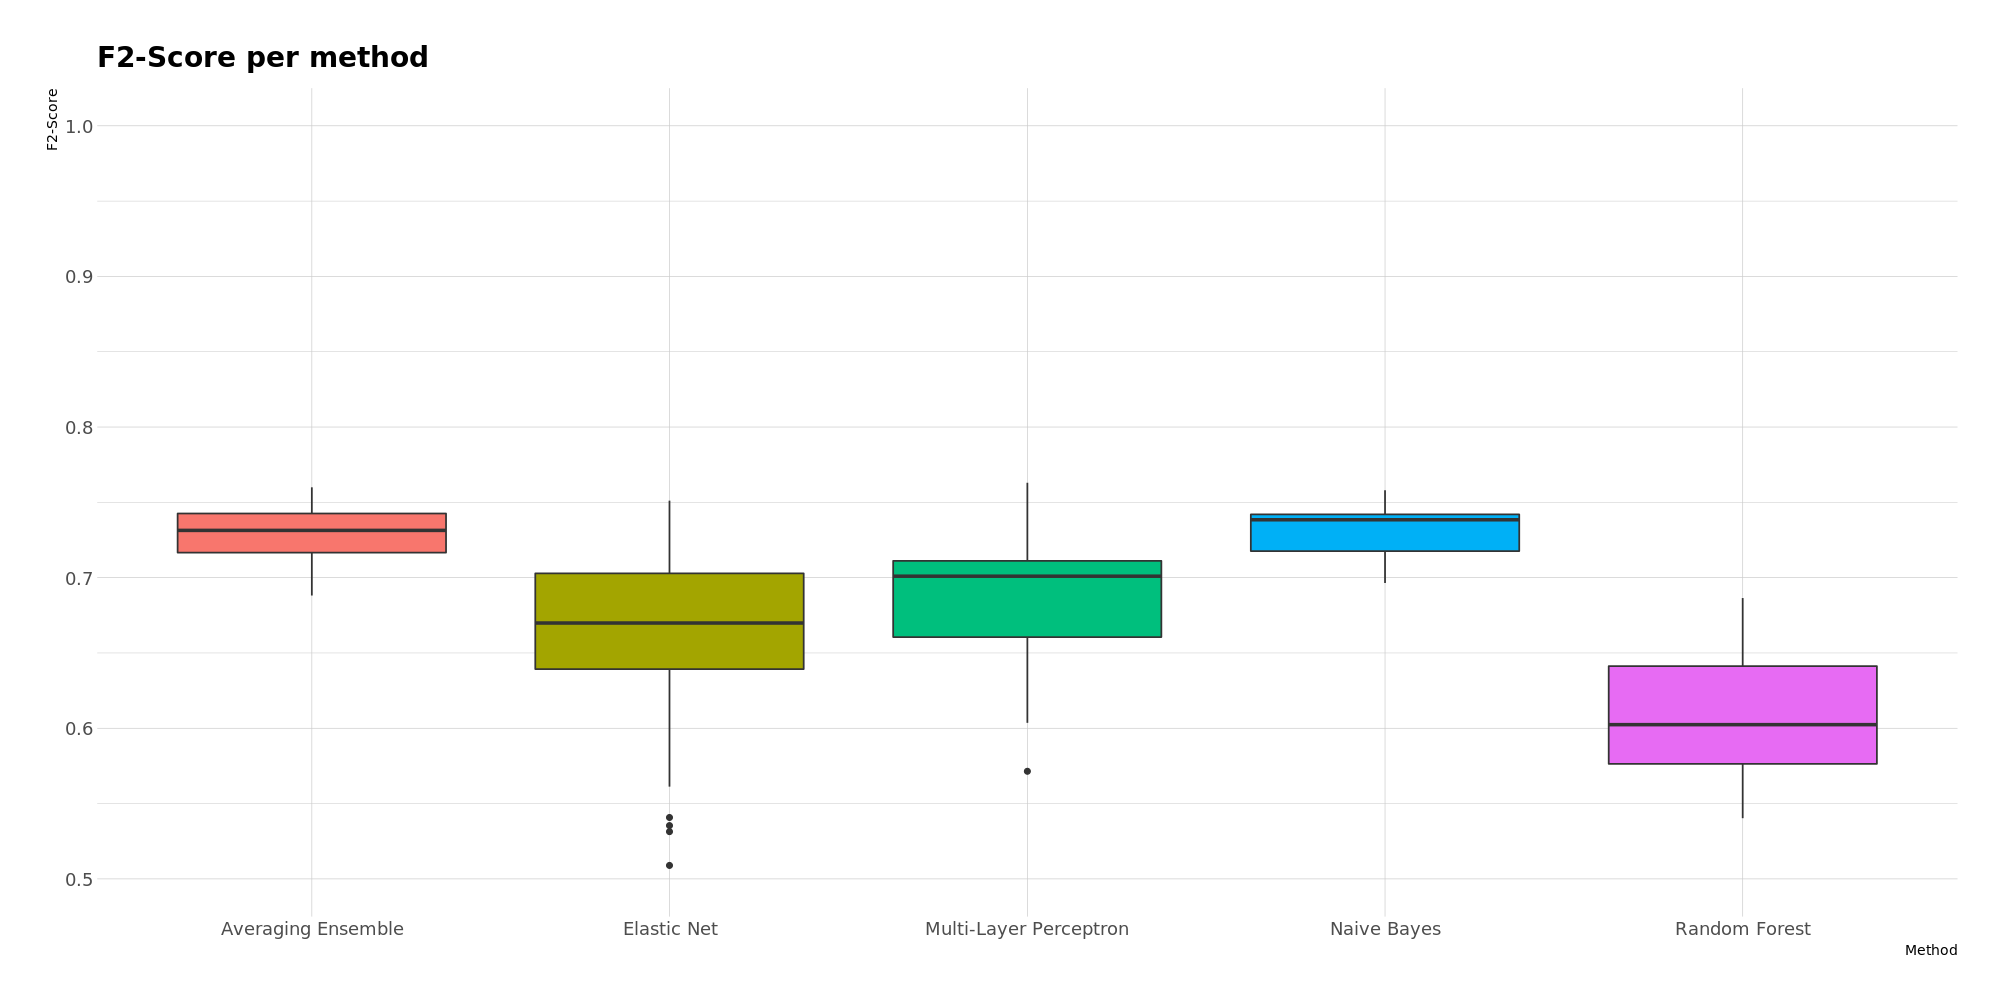
\includegraphics[scale=.2]{../reports/results/models_and_evals/summary/box_plot_f2.png}}
    \label{fig:boxplot-f2}
\end{figure}

\begin{figure}[H]
    \caption{Comparison of measured AUCROC for different algorithms}
    \centerline{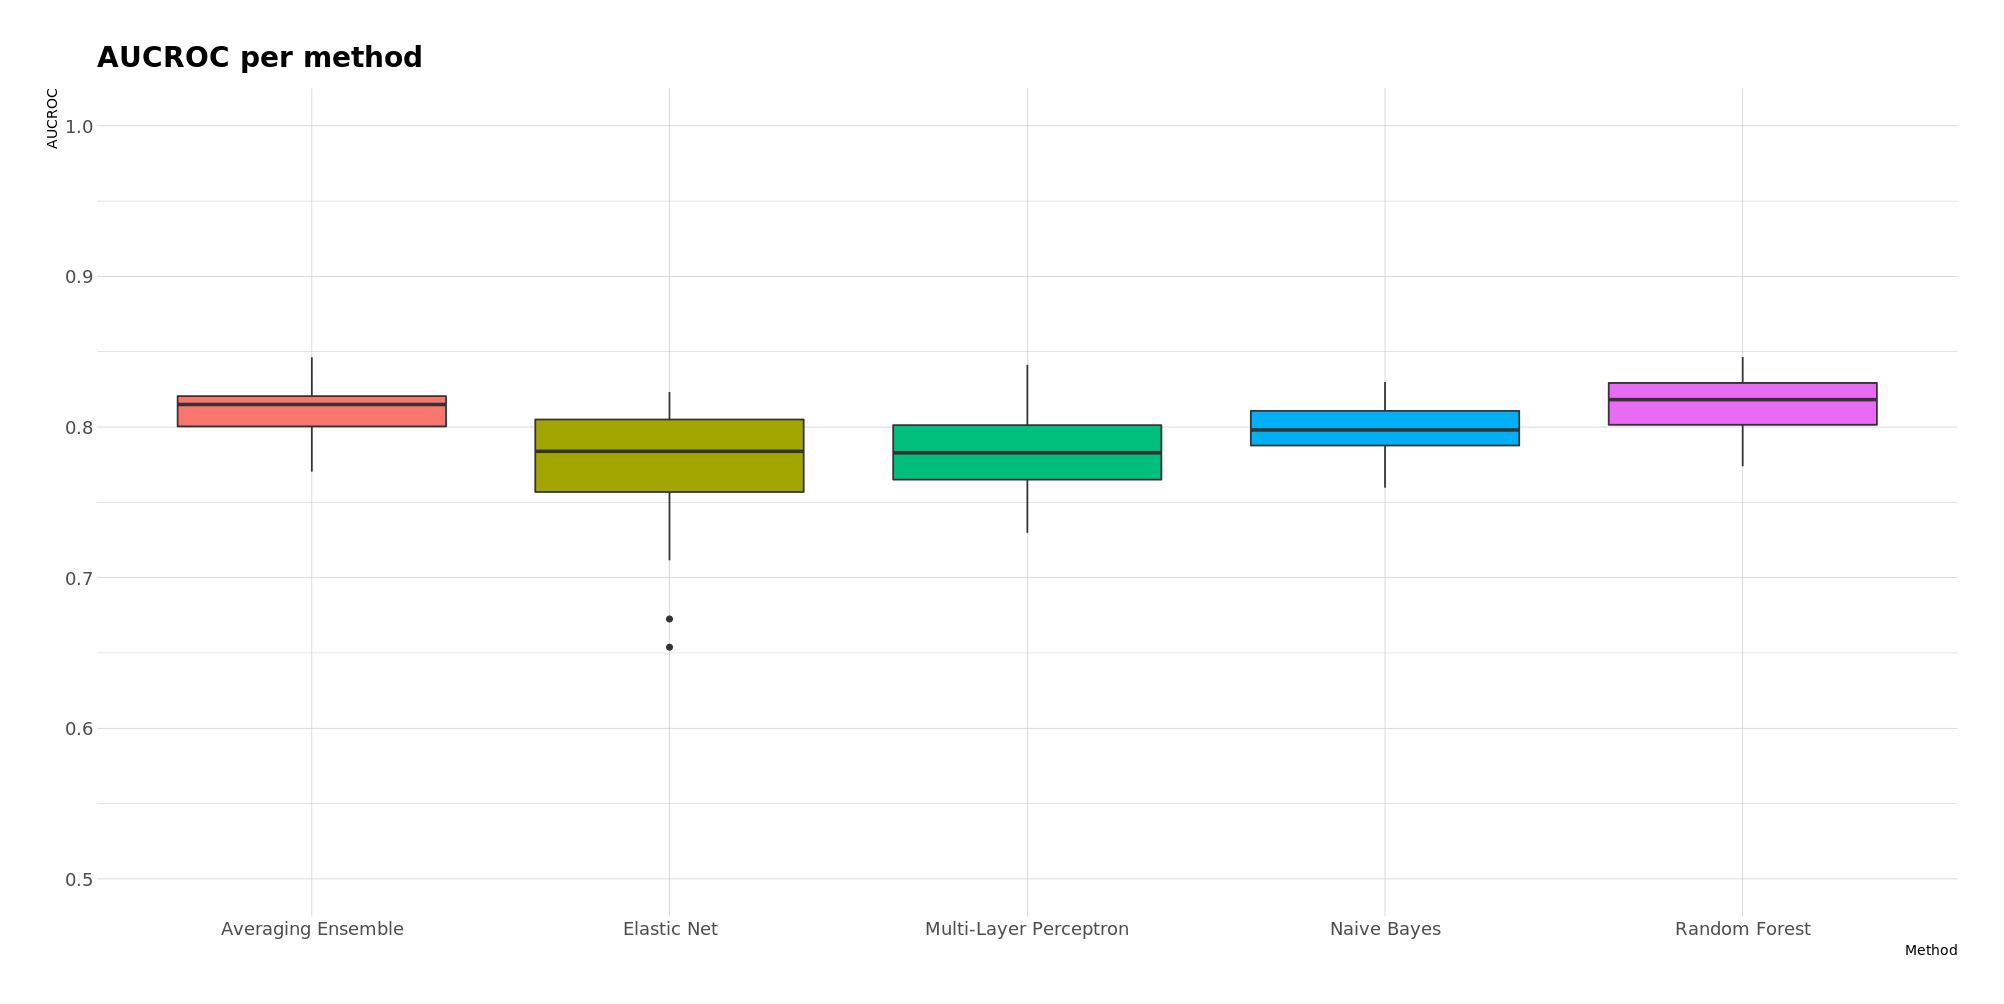
\includegraphics[scale=.2]{../reports/results/models_and_evals/summary/box_plot_aucroc.png}}
    \label{fig:boxplot-aucroc}
\end{figure}

\begin{figure}[H]
    \caption{Comparison of measured sensibility for different algorithms}
    \centerline{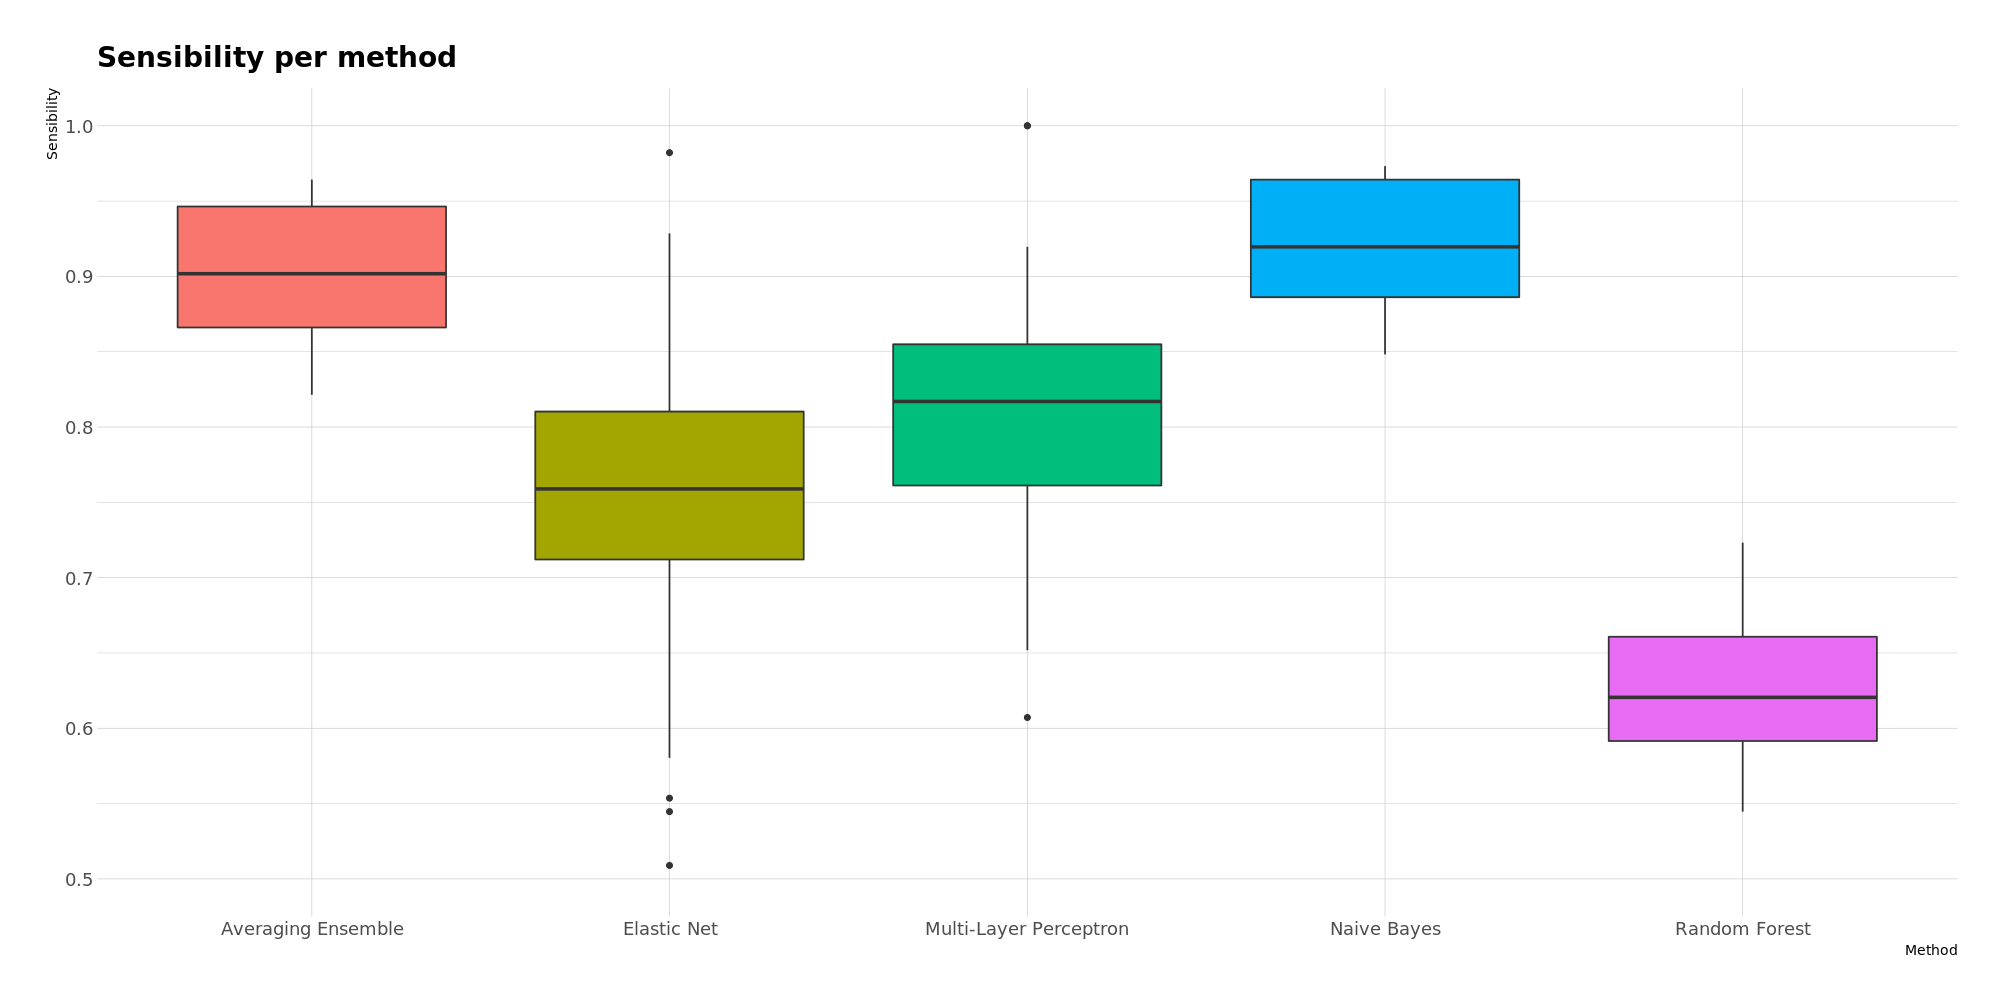
\includegraphics[scale=.2]{../reports/results/models_and_evals/summary/box_plot_sens.png}}
    \label{fig:boxplot-sens}
\end{figure}

\begin{figure}[H]
    \caption{Comparison of measured specificity for different algorithms}
    \centerline{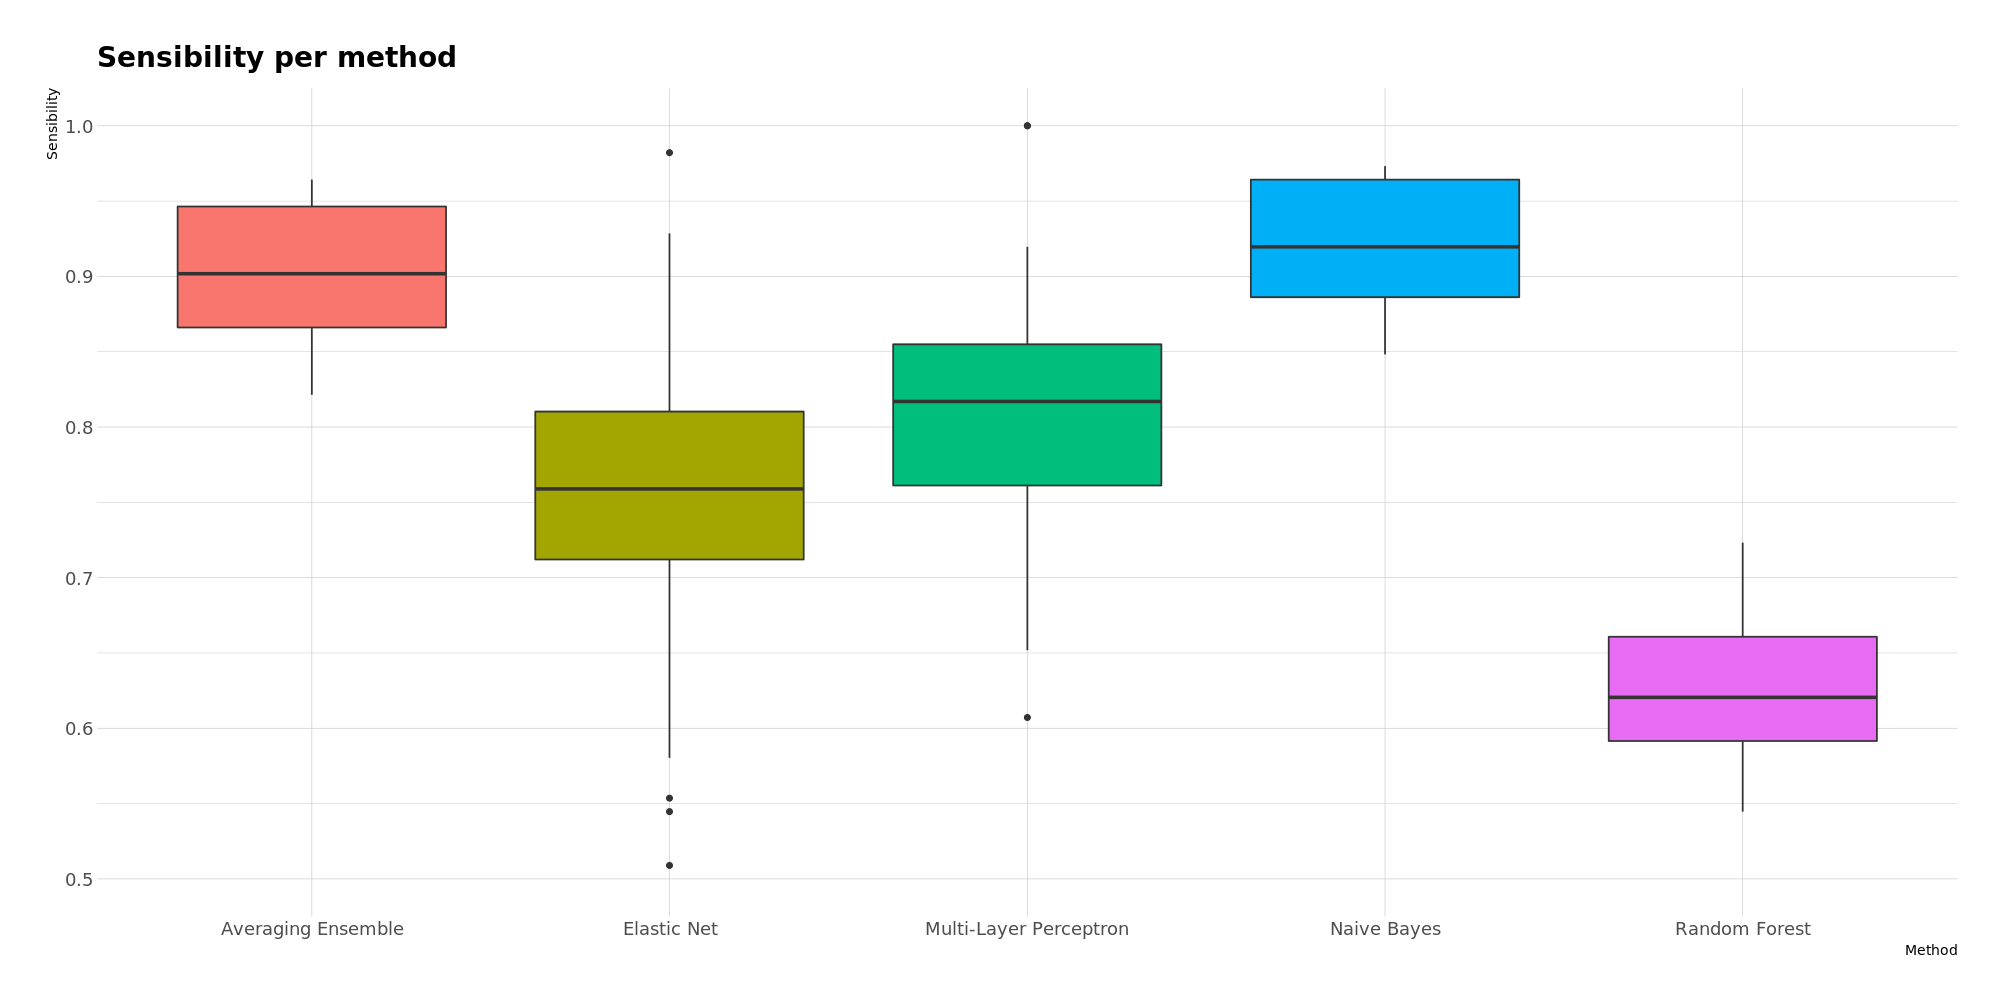
\includegraphics[scale=.2]{../reports/results/models_and_evals/summary/box_plot_spec.png}}
    \label{fig:boxplot-spec}
\end{figure}

\subsection{Hyperparameters Analysis}\label{subsec:hyperparameters-analysis}

\begin{table}[h]
    \caption{Hyperparameters most-frequently chosen in tuning}
    \begin{center}
        \begin{tabular}{l|c}
            \textit{Parameter}                    & \textit{Value}      \\
            \hline
            \hline
            Elastic Net - Alphas                  & 0.1                 \\
            Elastic Net - Lambda                  & 0.09                \\
            Neural Network - Layer 1 \#Units      & 1                   \\
            Neural Network - Layer 2 \#Units      & 1                   \\
            Random Forest - Node-splitting method & \textit{extratrees} \\
            Random Forest - \#Random-attributes   & 2                   \\
            \hline
        \end{tabular}
    \end{center}
    \label{tab:most-frequent-hyperparams}
\end{table}

For the analysis of the produced models internal characteristics, it is proper to first verify the results of the hyperparameters tuning process, as this plays an important role in models' performance.
The most frequently chosen hyperparameters values of the final models are summarized in Table~\ref{tab:most-frequent-hyperparams} and indicate that, in general, relatively simpler models tend to perform better in the training phase.
This is not surprising, since the best sizes of variables subsets are low and in the hyperparameters tuning phase the available data has a relatively small number of instances, thus it is probably the case the more complex models could overfit and perform poorly.

Figures~\ref{fig:params-ranger},~\ref{fig:params-mlp}, and ~\ref{fig:params-glmnet} show plots of the F\textsubscript{2}-Score during the training of the base-learners' model of a given resample, for multiple combinations of parameters of RFs, ANNs, and ENs (respectively).
We see that, at least for this fold (and we keep the graphical analysis limited to this single one for the sake of simplicity), performance estimates seem to vary in an orderly manner throughout the hyperparameter values planes.
More specifically, clear patterns are identifiable in every hyperparameters plot.

First, in the RF graph of Figure~\ref{fig:params-ranger}, where the \textit{extratrees} (extremely randomized trees) and the \textit{gini} tree-node-splitting methods are compared, we find that there is a big in the F\textsubscript{2}-Score between the two, but for both we observe relatively flat lines for higher values of randomly selected predictors (\textit{NRand}).
For the lower values (i.e.\ from the range between 2 and 20), with the increasing number of predictors, F\textsubscript{2}-Score increases in the \textit{gini} line, but decreases for the extremely randomized trees splitting method.
Most notably, the peak score is found in the left-most point of the \textit{extratrees} line.

\begin{figure}[H]
    \caption{Hyperparameter tuning for Random Forest in first CV resample}
    \centerline{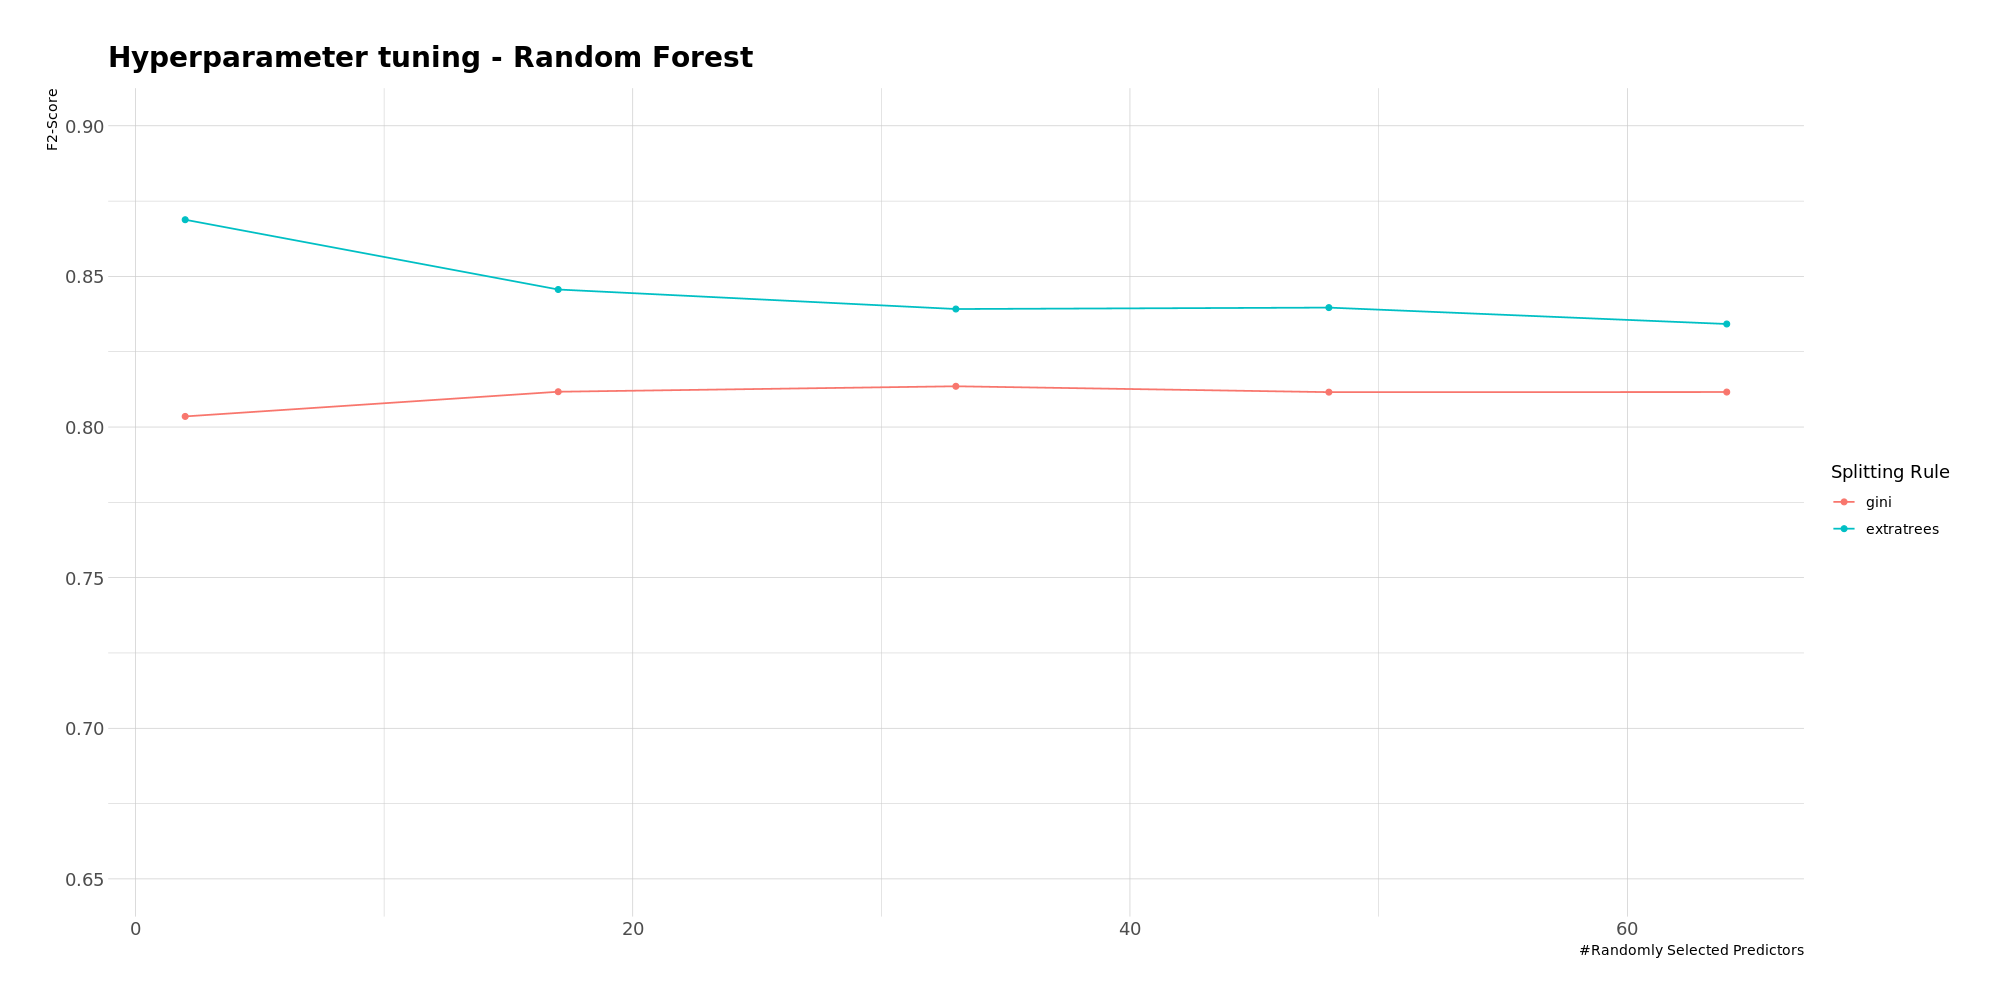
\includegraphics[scale=.21]{../reports/results/models_and_evals/summary/params_ranger_resample_1.png}}
    \label{fig:params-ranger}
\end{figure}

\begin{figure}[H]
    \caption{Hyperparameter tuning for Multilayer Perceptron in first CV resample}
    \centerline{\includegraphics[scale=.21]{../reports/results/models_and_evals/summary/params_mlpML_resample_1.png}}
    \label{fig:params-mlp}
\end{figure}

\begin{figure}[H]
    \caption{Hyperparameter tuning for Elastic Net in first CV resample}
    \centerline{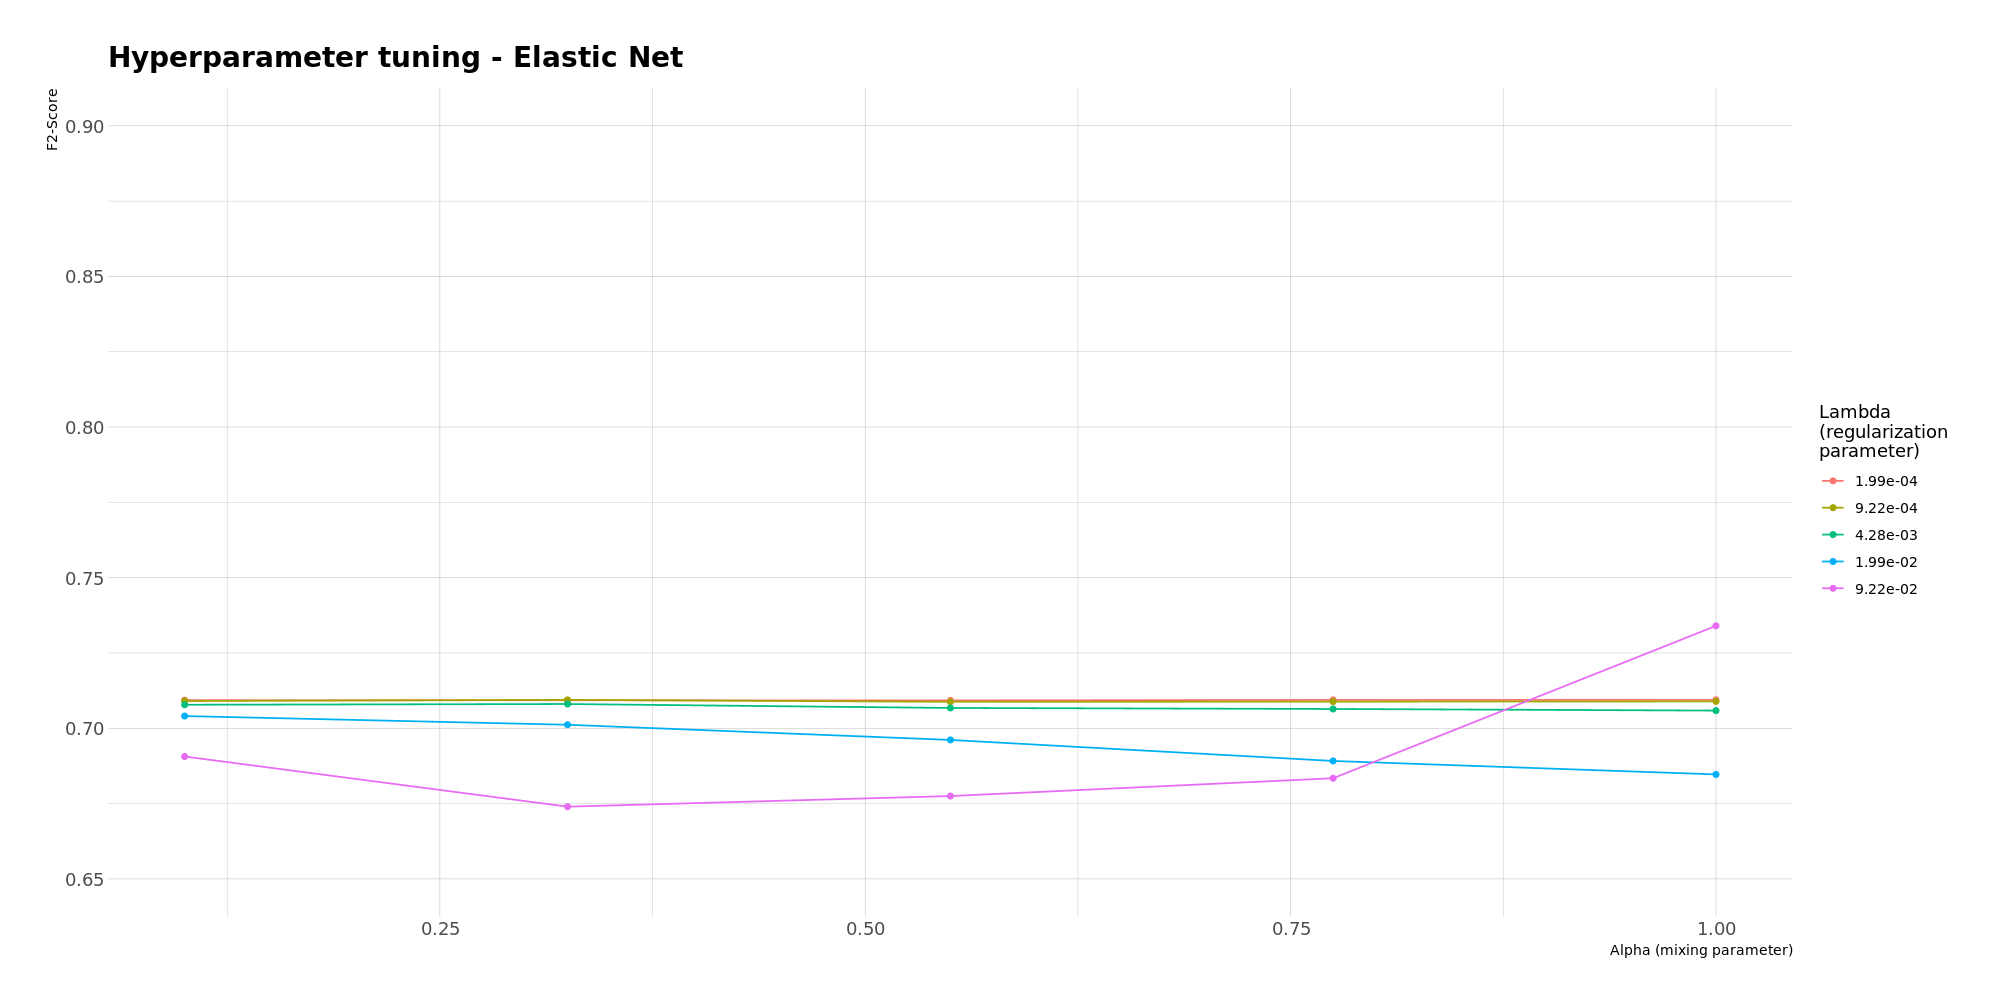
\includegraphics[scale=.21]{../reports/results/models_and_evals/summary/params_glmnet_resample_1.png}}
    \label{fig:params-glmnet}
\end{figure}

As for Figure~\ref{fig:params-mlp}, every colored line represents a neural network with a given number of neurons in the second (and last) hidden layer.
The commonalities between these slightly different architectures is that performance is lower for higher numbers of hidden units of layer 1 (although it varies in a bowl-shaped curve).
Increasing the number of neurons in layer 2 has a similar effect.
In other words, simpler ANNs, in our scenario, seem to carry out a better classification.

Lastly, the plot of EN's hyperparameters of Figure~\ref{fig:params-glmnet} indicates a similar behavior to the one seen for the random forest, in the sense that each line generally presents just small variations of F\textsubscript{2}-Score with respect to the variable from the horizontal axis (the lasso-ridge mixing parameter alpha in this case).
Also in the same manner as the RF's grid search, the maximum performance of this particular elastic net was achieved in an "extreme" value, the highest \textit{lambda} and highest \textit{alpha} pair (as it is with the lowest RF's \textit{NRand}).
This is curious to notice, as an \textit{alpha} value of 1 indicates a purely lasso regression.

\subsection{Feature Selection Analysis}\label{subsec:feature-selection-analysis}

Besides hyperparameters tuning, another characteristic worth examining is the models' predictive capabilities across different predictor sets of the RFE loops.
For each final RFE model produced, Figures~\ref{fig:rfe-glmnet},~\ref{fig:rfe-mlp}, and~\ref{fig:rfe-ranger} show the F\textsubscript{2}-Score variation depending on the number of variables considered in the base learners induction.
To analyse the algorithms' performance according to distinct features set sizes, it is useful to start the analysis of the results by the right side of the graph, which represents the original features set size.
This last mark in the horizontal axis indicates the data has as many variables as the cleansed dataset, which are then reduced in quantity down to about 600 by the base learners preprocessing.
As the RFE retrains and reassesses the variables importances at each iteration, the difference between the number of predictors before and after preprocessing should drastically diminish.
It is curious that both elastic nets (Figure ~\ref{fig:rfe-glmnet}) and ANNs (~\ref{fig:rfe-mlp}) tend to perform better with fewer variables, showing a smoothly varying F\textsubscript{2}-Score curve.
On the other hand, random forests present a performance peak at the predictor set size of 64 (Figure~\ref{fig:rfe-ranger}), which indicates that after further removal of variables, too much valuable information is taken out from the model training process.

\begin{figure}[H]
    \caption{Recursive feature elimination performance for Elastic Net}
    \centerline{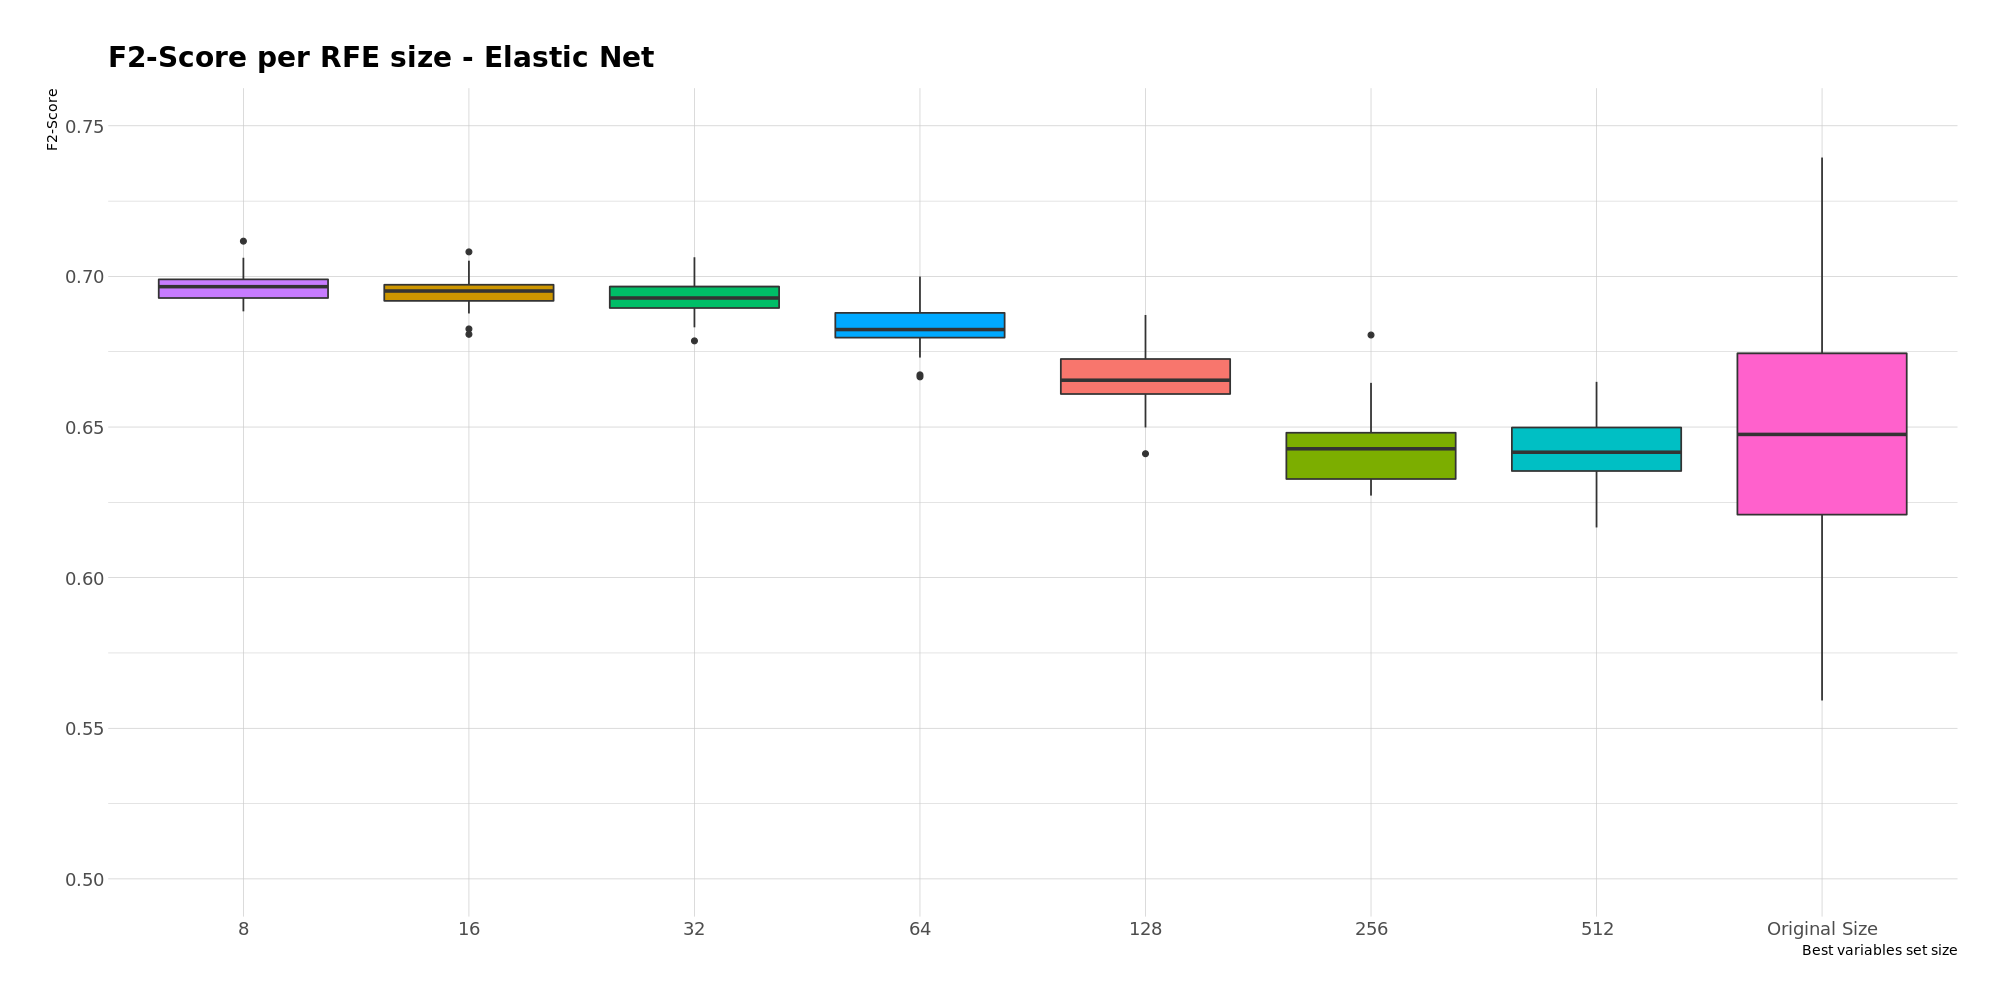
\includegraphics[scale=.21]{../reports/results/models_and_evals/summary/rfe_glmnet.png}}
    \label{fig:rfe-glmnet}
\end{figure}

\begin{figure}[H]
    \caption{Recursive feature elimination performance for Multilayer Perceptron}
    \centerline{\includegraphics[scale=.21]{../reports/results/models_and_evals/summary/rfe_mlpML.png}}
    \label{fig:rfe-mlp}
\end{figure}

\begin{figure}[H]
    \caption{Recursive feature elimination performance for Random Forest}
    \centerline{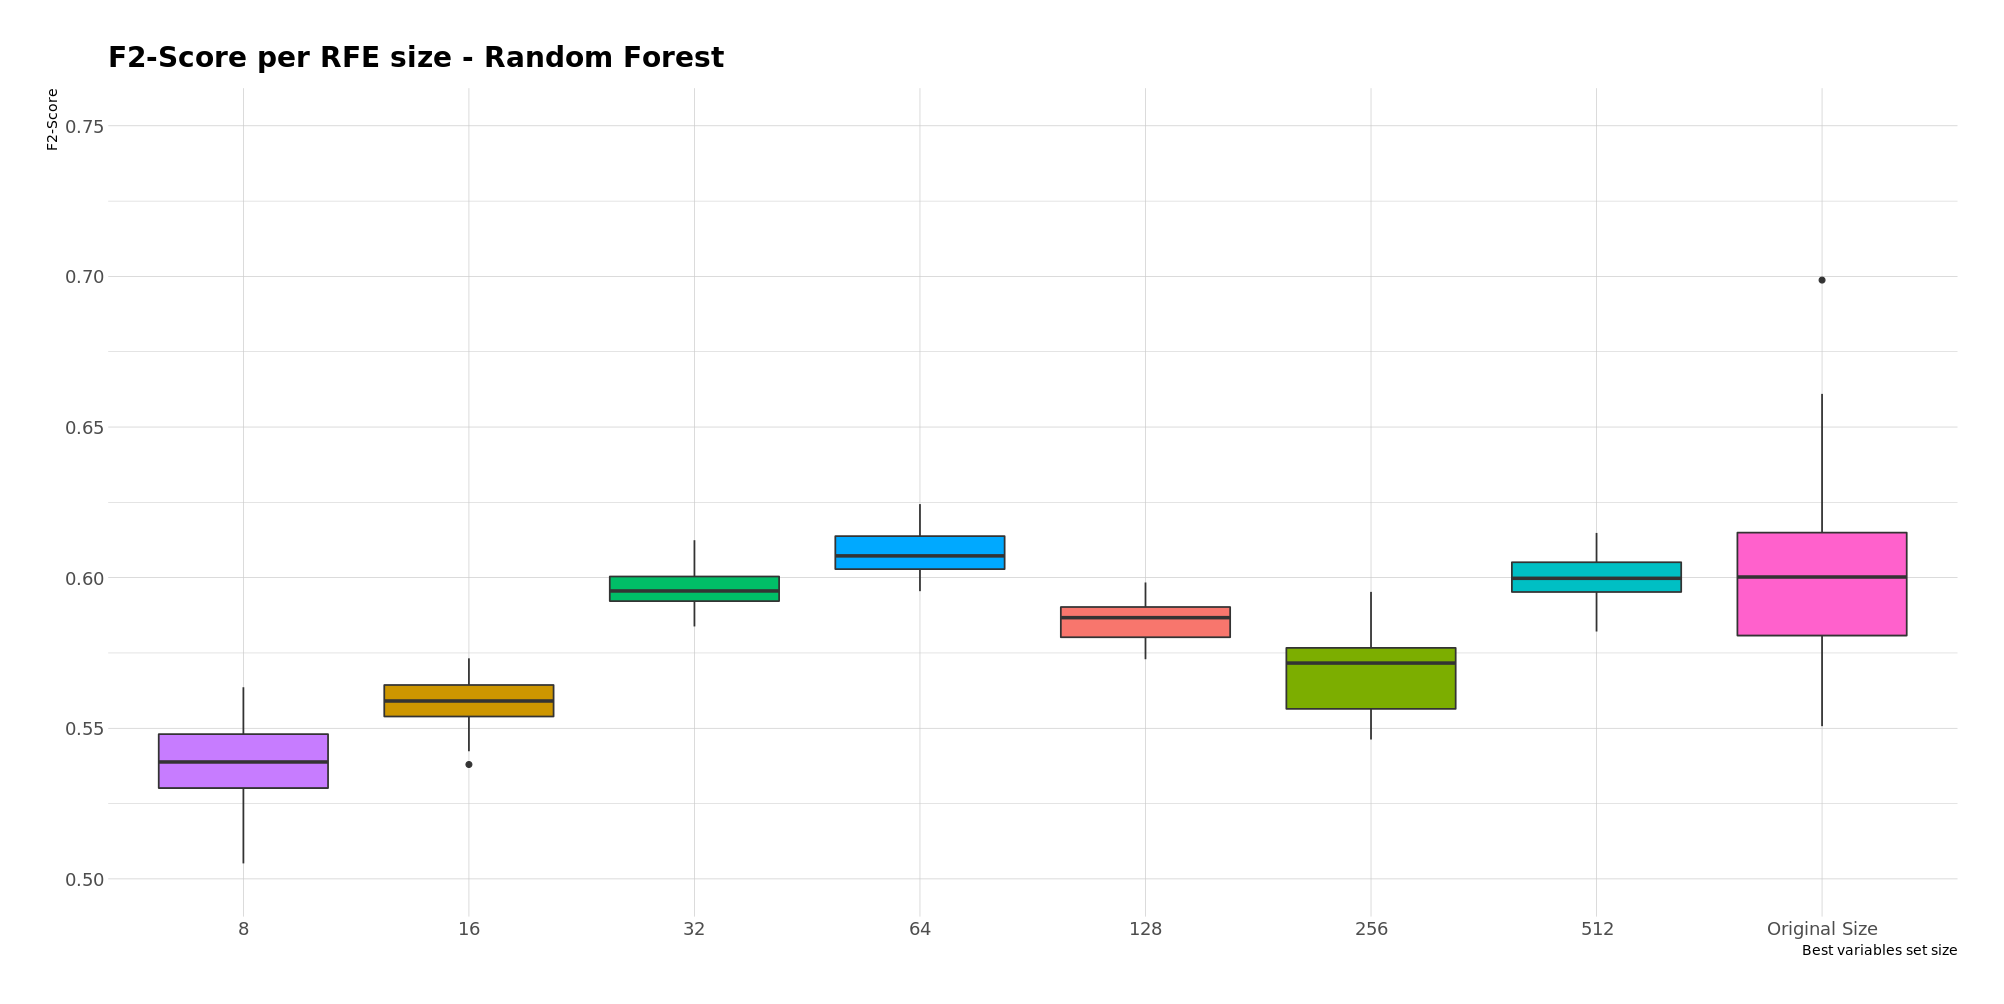
\includegraphics[scale=.21]{../reports/results/models_and_evals/summary/rfe_ranger.png}}
    \label{fig:rfe-ranger}
\end{figure}

To analyse the rankings of features importances for each algorithm, we produced "rank matrices" that can be plotted as heatmaps shown in Figures ~\ref{fig:heatmap-glmnet},~\ref{fig:heatmap-mlp}, and ~\ref{fig:heatmap-ranger}.
The idea of this visualization approach is the following: each predictor (in the vertical axis, ordered alphabetically for a naive semantical clustering) has its importance mapped to each of the trained models (with a 1:1 correspondence to a CV resample) by a ranking function \textit{F\textsubscript{rank}}.
The complete list of meanings of the top-30 most relevant attributes found using each algorithm is available in Table~\ref{tab:most-important-variables}.
The value of each attribute-to-model cell is zero when the variable does not appear in the list of most important predictors of the model.
Otherwise, it is defined as follows (where \textit{A\textsubscript{m}} is the set of best attributes of a model \textit{m}, and \textit{I(a, m)} is the index of the attribute \textit{a} in \textit{A\textsubscript{m}}):

\begin{equation}
    F_{rank}(a, m) = \frac{\#A_m - I(a, m)}{\#A_m}
\end{equation}

Our attribute-rank matrices then have higher values (indicated by brighter colors in the heatmaps) for the variables that are most important, but the magnitudes are relatively decreased given a fixed rank index for models that have larger best-variables sets.
Moreover, the values of these matrices range from 0 to 1 after normalization according to the variables sets sizes.
Thus, the intuitions to be derived from the heatmap plots of these matrices are that horizontal lines show how the feature relevances vary across the collection of trained models, and clusters of horizontal lines with uniform colors indicate the importance of semantically similar attributes.

For each algorithm, we can average the \textit{F\textsubscript{rank}}s of each predictor across the multiple resamples to obtain generalized variable importances.
More precisely, we calculate what we define as \textit{G\textsubscript{imp}(a)} (the general importance of an attribute \textit{a}), based on a set of models \textit{M}, as:

\begin{equation}
    G_{imp}(a) = \sum_{n=1}^{\#M} \frac{F_{rank}(a,m)}{\#M}
\end{equation}

In Figures ~\ref{fig:heatmap-glmnet},~\ref{fig:heatmap-mlp}, ~\ref{fig:heatmap-ranger}, we displayed only the top-30 \textit{G\textsubscript{imp}} features.
We chose 30 because it matches the number of resamples in this plot, yielding a more pleasant plot aesthetic, but most importantly because it is a sufficient and efficient size for a set of best variables to be considered in our analysis, in the sense that we do not need to discuss many predictors but the ones we discuss are relevant and insightful (especially given the best attribute sizes indicated in Figures~\ref{fig:rfe-glmnet},~\ref{fig:rfe-mlp} and~\ref{fig:rfe-ranger}).

The exception of this rule is Figure~\ref{fig:heatmap-mlp}, where only 17 features are shown.
We note that, for this algorithm, there are also relatively clearer horizontal and vertical patterns in the heatmap, and also low variance in its RFE plot (Figure~\ref{fig:rfe-mlp}).
This indicates that these models are more concise, and also homogeneous between each other.

\begin{figure}[H]
    \caption{Heatmap of attribute relevance for Elastic Net}
    \centerline{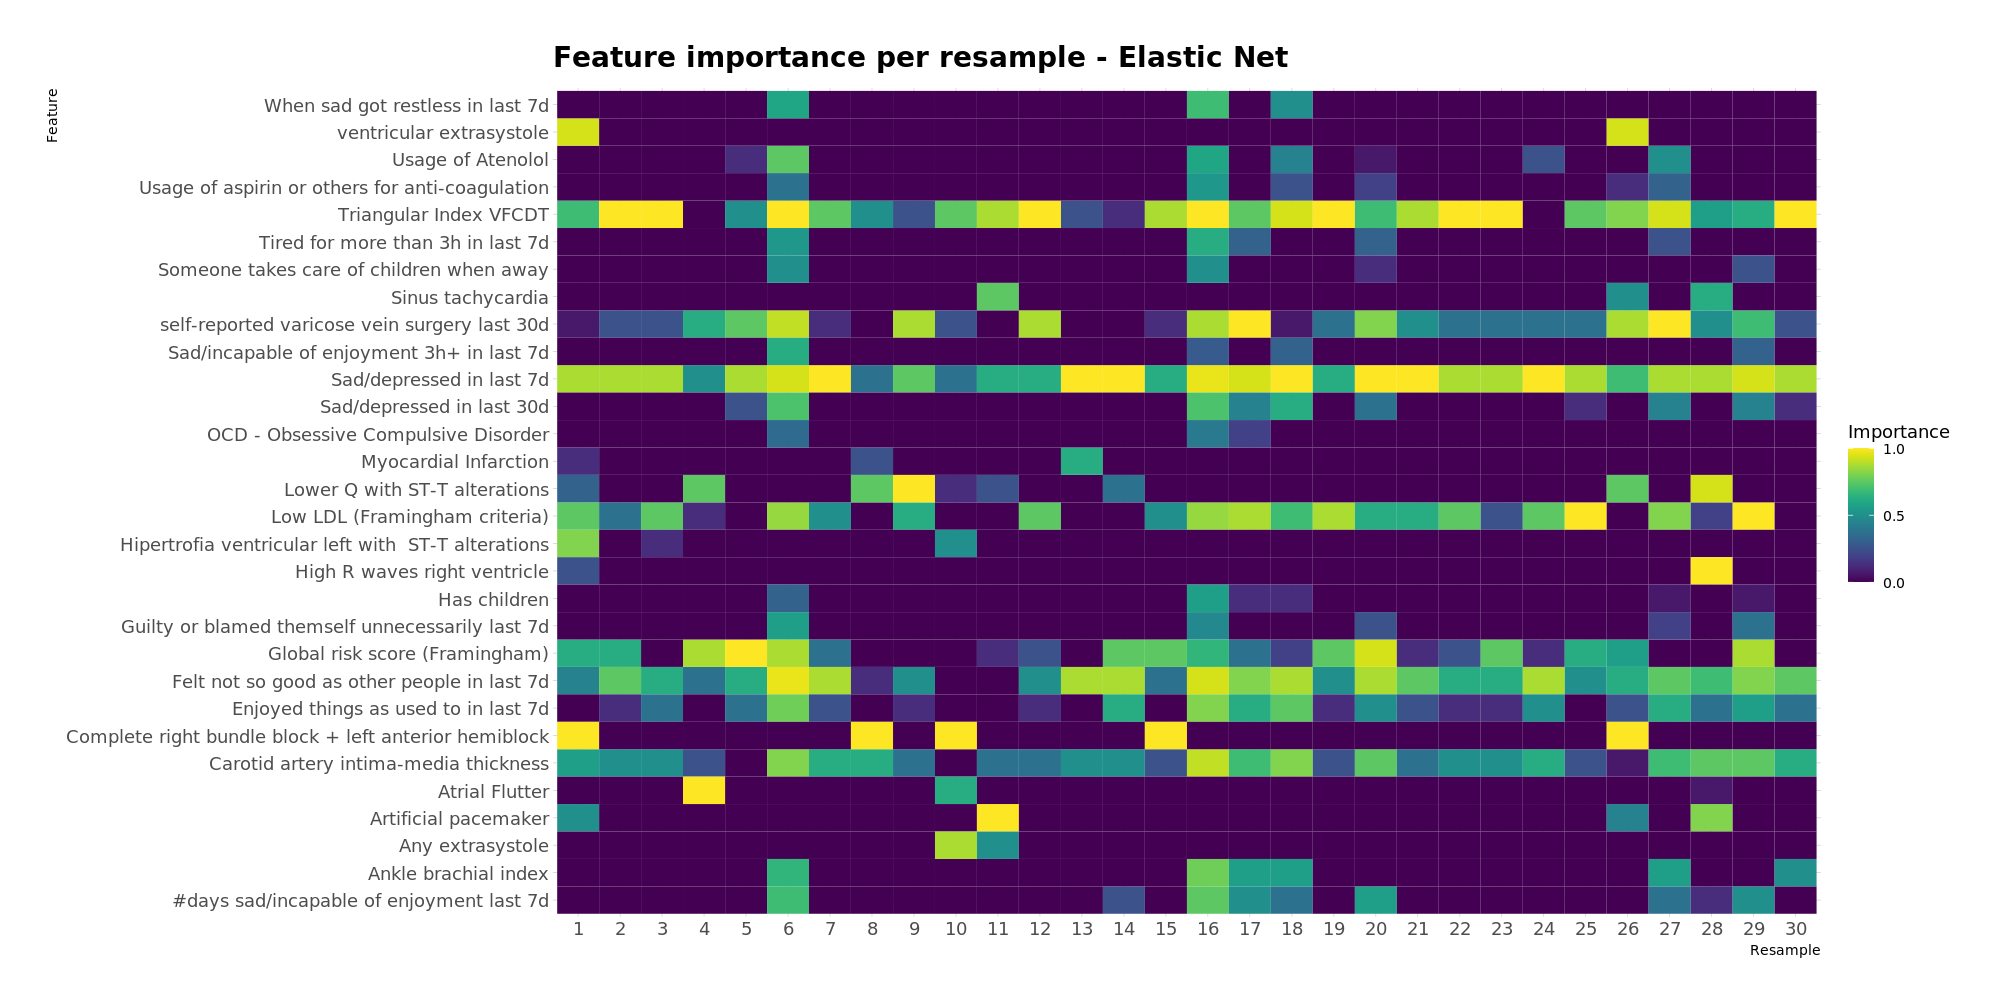
\includegraphics[scale=.21]{../reports/results/models_and_evals/summary/var_imp_resample_glmnet.png}}
    \label{fig:heatmap-glmnet}
\end{figure}

\begin{table}[H]
    \renewcommand{\arraystretch}{0.65} % Default value: 1
    \caption{Variables ranked as most important for trained models in alphabetical order}
    \begin{center}
        \begin{tabular}{l|l}
            \textit{Attribute}                & \textit{Description}                                  \\
            \hline
            \hline
            bp\_derivedA\_RAZAOPAS            & Ankle brachial index                                  \\
            cisab5                            & Tired for more than 3h in last 7d (B5)                \\
            cisae7                            & Argument fight in last 7d (E7)                        \\
            cisag1                            & Sad/depressed in last 30d (G1)                        \\
            cisag2                            & Enjoyed things as used to in last 30d (G2)            \\
            cisag4                            & Sad/depressed in last 7d (G4)                         \\
            cisag5                            & Enjoyed things as used to in last 7d (G5)             \\
            cisag6                            & \#days sad/incapable of enjoyment last 7d (G6)        \\
            cisag7                            & Sad/incapable of enjoyment 3h+ in last 7d (G7)        \\
            cisah1                            & Worst time of day for sadness last 7d (H1)            \\
            cisah2                            & Sexual desire in last 30d (H2)                        \\
            cisah3a                           & When sad, got restless in last 7d (H3a)               \\
            cisah3b                           & When sad, did things more slowly in last 7d (H3b)     \\
            cisah3c                           & When sad got less talkative in last 7d (H3c)          \\
            cisah4                            & Guilty or blamed themself unnecessarily last 7d (H4)  \\
            cisah5                            & Felt not so good as other people in last 7d (H5)      \\
            cisai8                            & How unpleasant was the worrying in last 7d (I8)       \\
            cisaj8                            & How unpleasant was the general anxiety last 7d (J8)   \\
            cisan1                            & Unpleasant thoughts kept appearing last 30d (N1)      \\
            cisao1                            & Feelings precluded things last 7d (O1)                \\
            cisao1a                           & Feelings precluded more than once last 7d (O1a)       \\
            derived\_A\_FRAMINGHAM\_CHD\_LDL  & Low LDL (Framingham criteria)                         \\
            derived\_A\_GLOBAL\_RISK          & Global risk score (Framingham)                        \\
            derived\_A\_RCPCIRVARIZESULT30D   & Self-reported varicose vein surgery in last 30d       \\
            derived\_A\_VIFA30\_PMCAT         & Familial income                                       \\
            derived\_cogA\_FLUENCIA\_LETRAF   & Fluency score with words with the letter F            \\
            derived\_nle                      & Any negative life event                               \\
            derived\_usga1                    & Carotid artery intima-media thickness                 \\
            EKG\_a\_ecgmc\_bcrd\_hae          & Complete right bundle block + left anterior hemiblock \\
            EKG\_a\_ecgmc\_esv                & ventricular extrasystole                              \\
            EKG\_a\_ecgmc\_fluttera           & Atrial Flutter                                        \\
            EKG\_a\_ecgmc\_hve\_stt           & Left ventricular hypertrophy with ST-T alterations    \\
            EKG\_a\_ecgmc\_im                 & Myocardial Infarction                                 \\
            EKG\_a\_ecgmc\_mp                 & Artificial pacemaker                                  \\
            EKG\_a\_ecgmc\_qmenor\_stt        & Lower Q with ST-T alterations                         \\
            EKG\_a\_ecgmc\_qualquer\_ex\_vent & Any extrasystole                                      \\
            EKG\_a\_ecgmc\_rvd                & High R waves right ventricle                          \\
            EKG\_a\_ecgmc\_ts                 & Sinus tachycardia                                     \\
            EKG\_a\_vfccl\_triangindex\_dt    & Triangular Index VFCDT                                \\
            home\_info\_vifa11                & Children (Q11)                                        \\
            meds\_atenolol                    & Usage of Atenolol                                     \\
            mentalvar\_\_TAG                  & GAD - Generalized Anxiety Disorder                    \\
            mentalvar\_\_TOC                  & OCD - Obsessive Compulsive Disorder                   \\
            mentalvar\_A\_SINTDEP             & Depression symptoms                                   \\
            mentalvar\_A\_SINTMEMORIA         & Concentration symptoms                                \\
            metadata\_ecga2                   & V4 value                                              \\
            negativelifeevents\_evea12        & Severe financial difficulties in last 12m (Q12)       \\
            neighborhood\_viza06              & Physical activities conditions in neighbourhood (Q6)  \\
            others\_cssa3                     & Usage of aspirin or others for anti-coagulation       \\
            others\_esca03                    & Work-related self-evaluation (Q3)                     \\
            social\_support\_capa57           & Someone takes care of children when away (Q57)        \\
            \hline
        \end{tabular}
    \end{center}
    \label{tab:most-important-variables}
\end{table}

\begin{figure}[H]
    \caption{Heatmap of attribute relevance for Multilayer Perceptron}
    \centerline{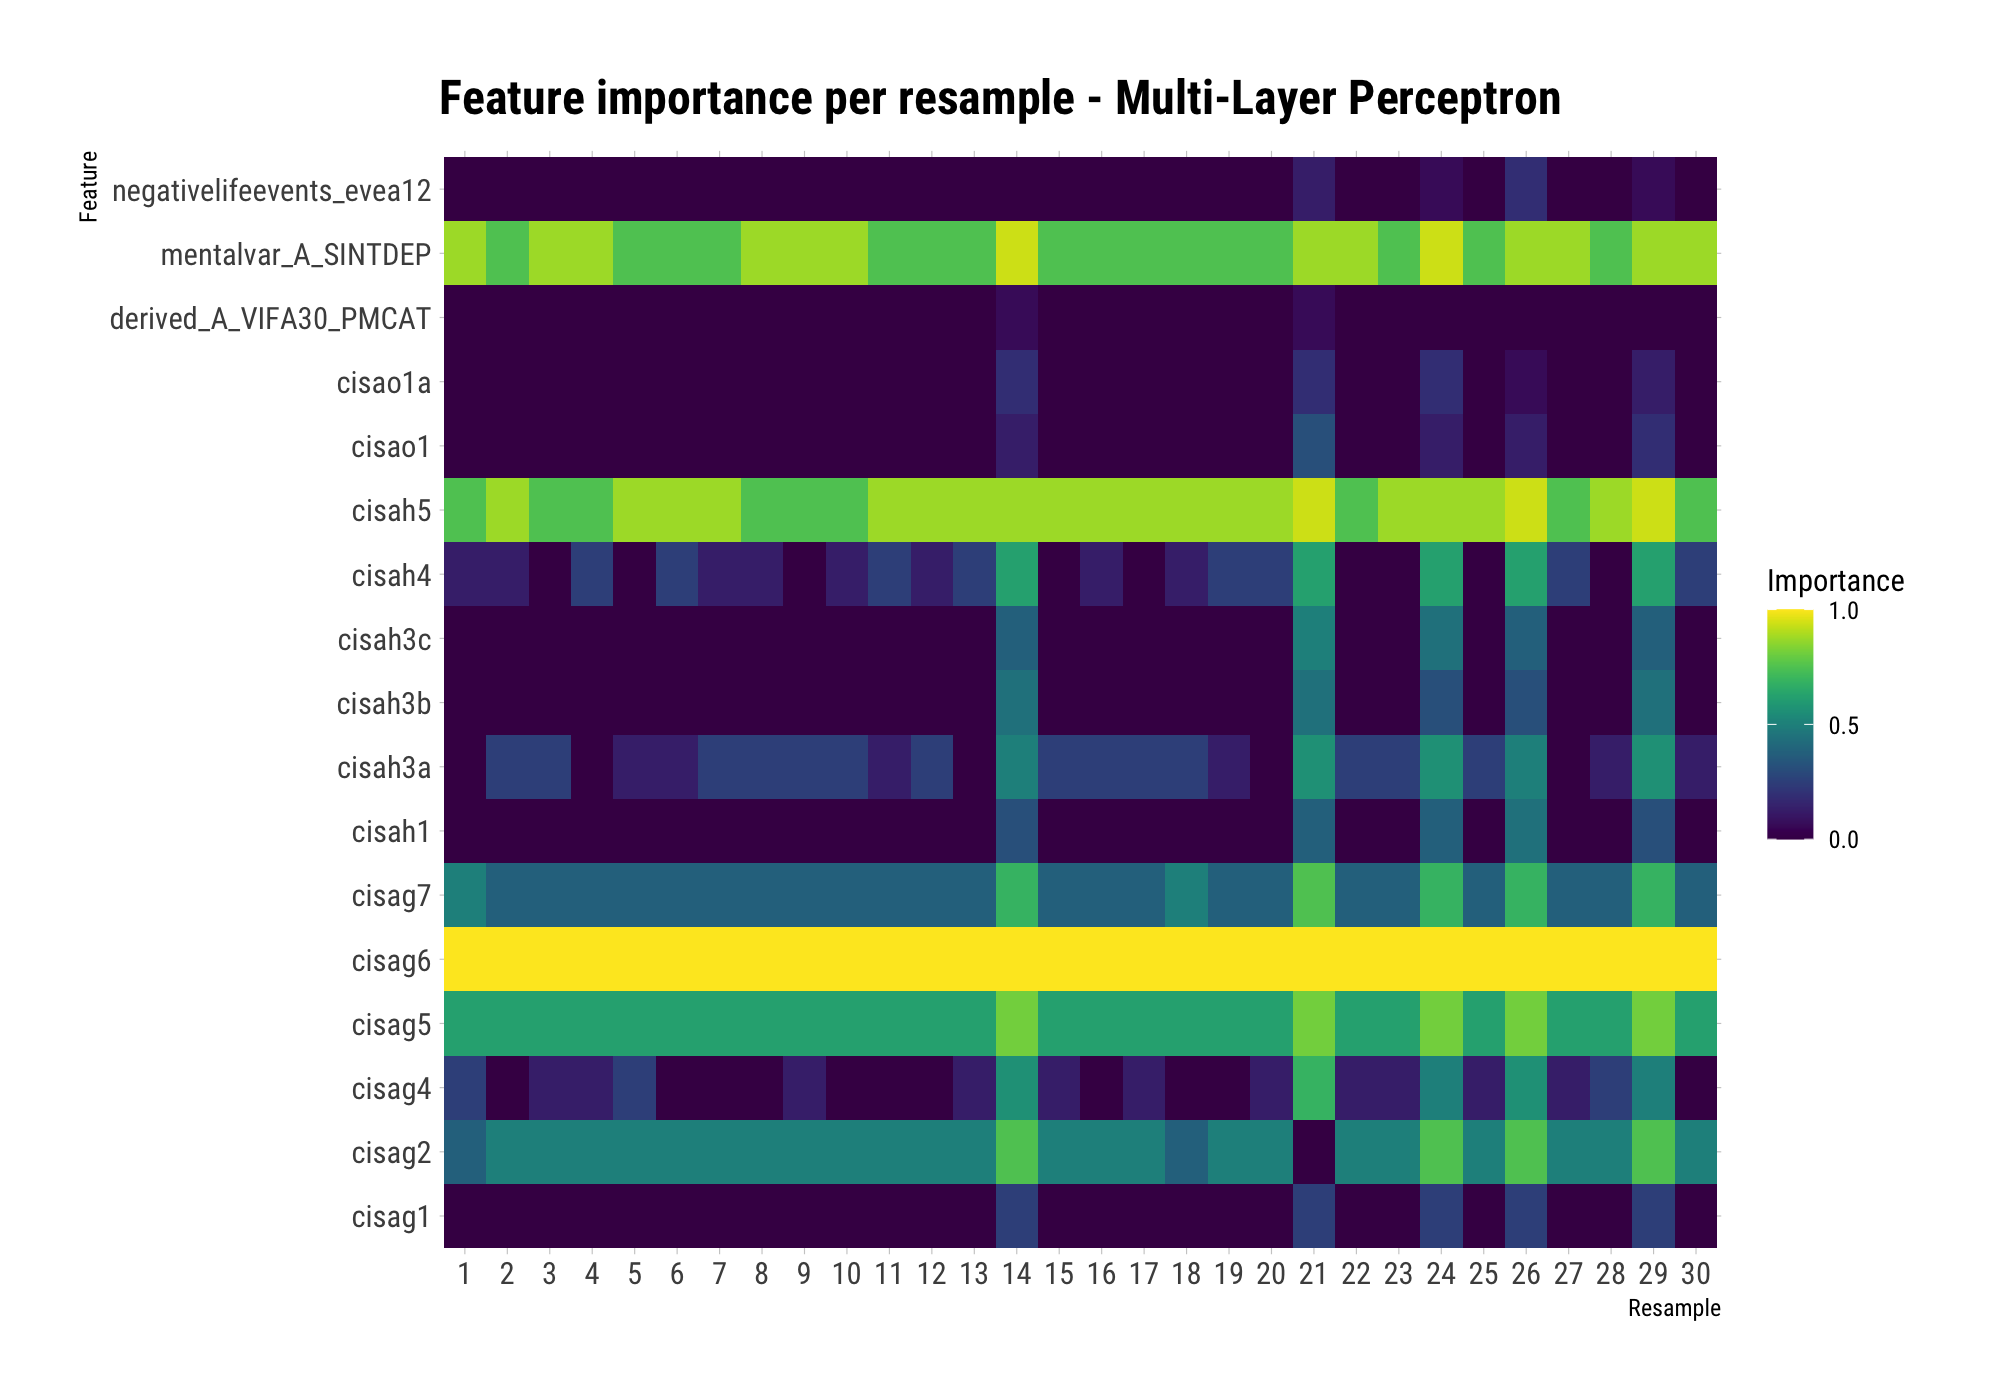
\includegraphics[scale=.21]{../reports/results/models_and_evals/summary/var_imp_resample_mlpML.png}}
    \label{fig:heatmap-mlp}
\end{figure}

\begin{figure}[H]
    \caption{Heatmap of attribute relevance for Random Forest}
    \centerline{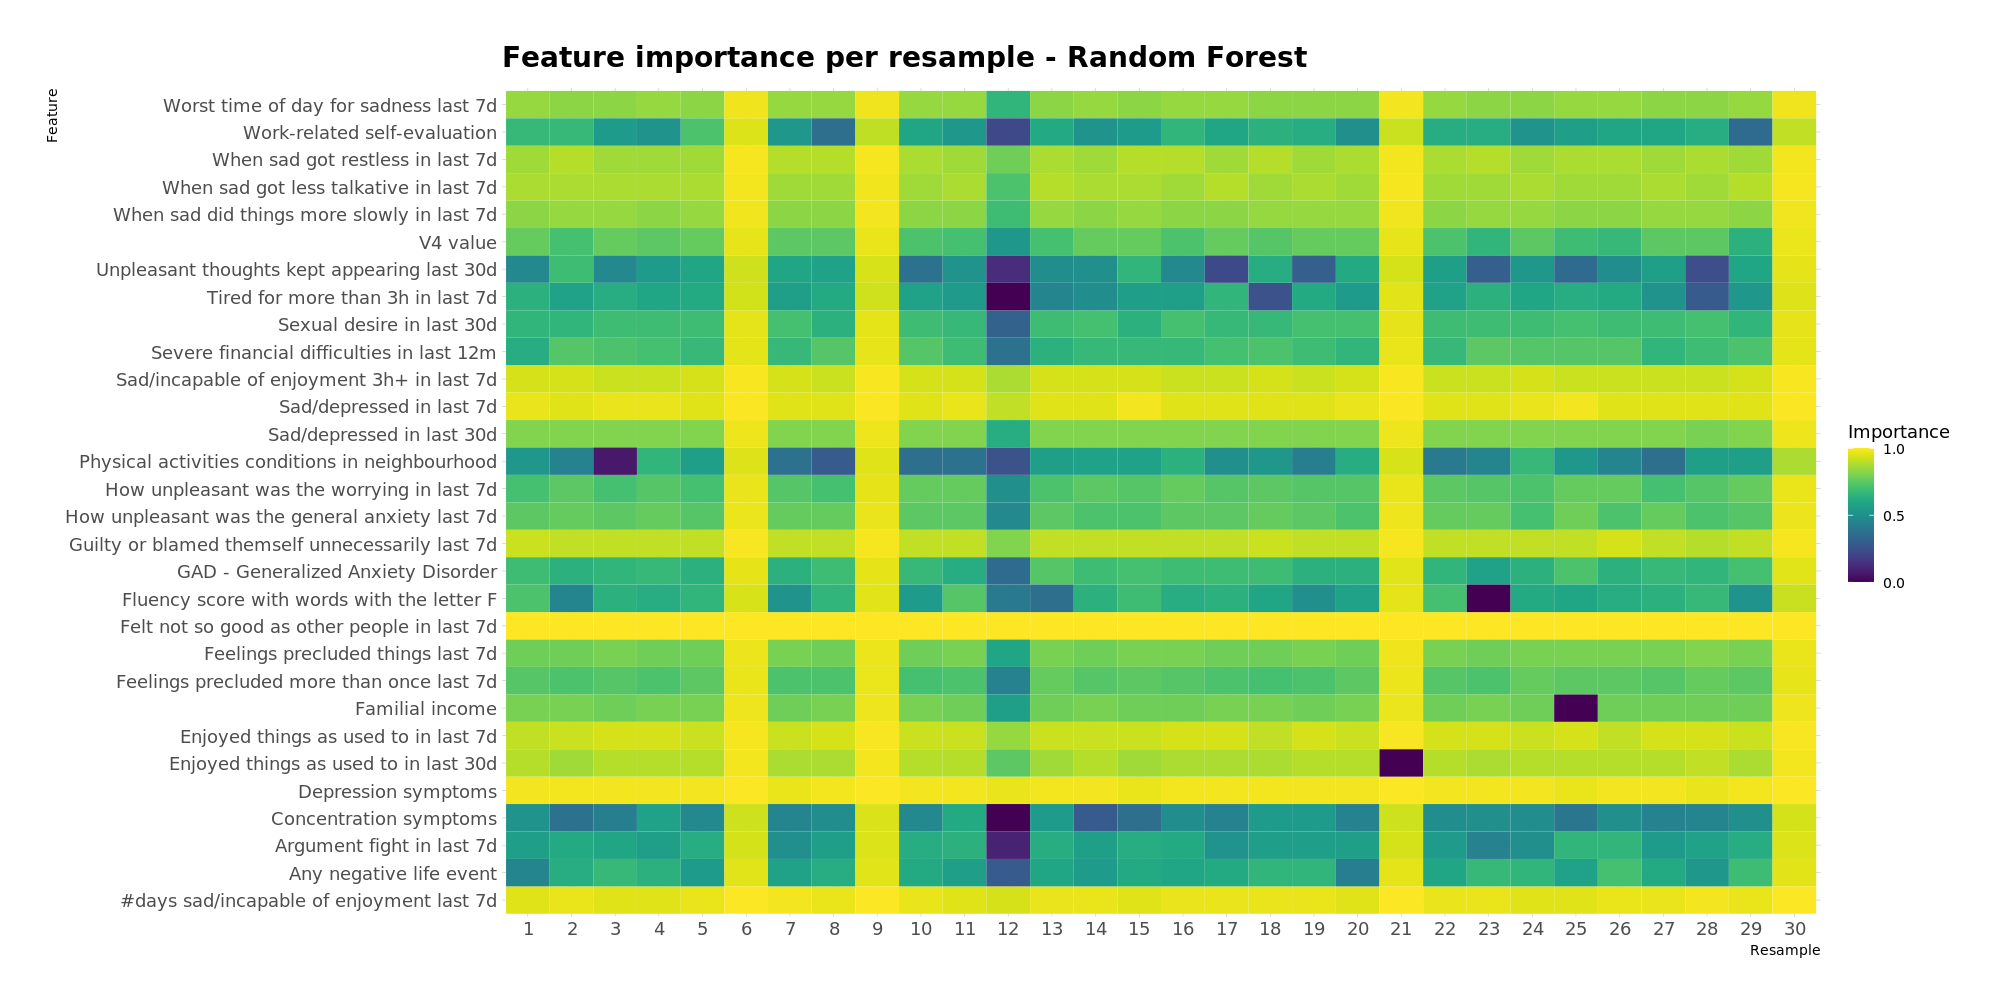
\includegraphics[scale=.21]{../reports/results/models_and_evals/summary/var_imp_resample_ranger.png}}
    \label{fig:heatmap-ranger}
\end{figure}

\pagebreak

Another useful employment of our \textit{G\textsubscript{imp}} metric is to arrange the variables according to it, ordered from highest to lowest, so that we can understand at a glance what each algorithm tends to consider most when predicting the classes of instances.
This is shown in Figures~\ref{fig:rank-glmnet},~\ref{fig:rank-mlp}, and~\ref{fig:rank-ranger}.

In diametrical opposition to the MLPs' simplicity, RFs learned that many more predictors are relevant for correct classification.
This is indicated by the already described performance peak at 64 RFE variables, by the \textit{F\textsubscript{rank}} heatmap (Figure ~\ref{fig:heatmap-ranger}) being overall brighter than the MLP's and EN's heatmaps, and by the top 30 attributes having small \textit{G\textsubscript{imp}} differences between each other (Figure ~\ref{fig:rank-ranger}).

On the other hand, based on the features heatmap and the rank plot of Figures~\ref{fig:heatmap-glmnet} and~\ref{fig:rank-glmnet}, we can place the elastic nets in an "intermediate" spot between the MLPs and the RFs regarding simplicity and homogeneity.
Figure~\ref{fig:heatmap-glmnet} indicates patterns of some features being considered relevant across different resamples, but the patterns are not so clear and uniform as the MLP's, and the variables are not so numerous or few as the RF's or MLP's, respectively.

\begin{figure}[H]
    \caption{Rank attribute relevance for Elastic Net}
    \centerline{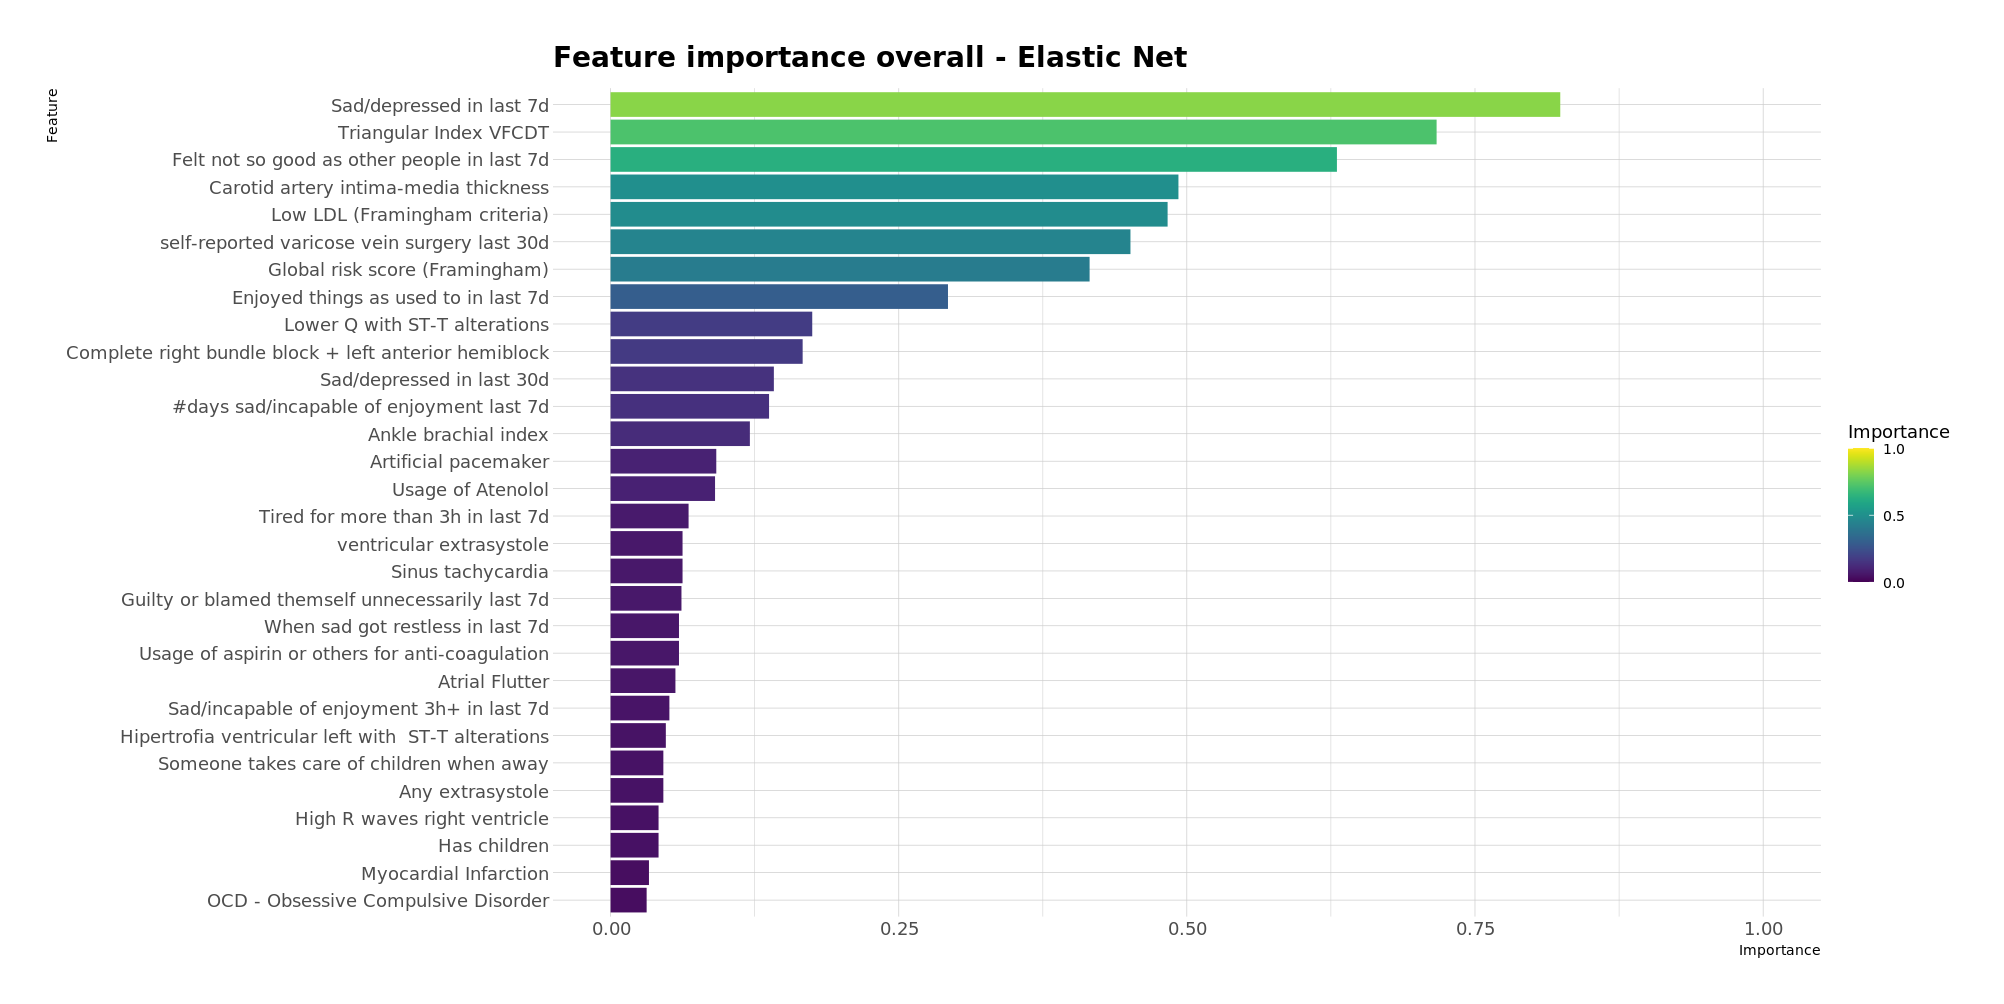
\includegraphics[scale=.21]{../reports/results/models_and_evals/summary/var_imp_glmnet.png}}
    \label{fig:rank-glmnet}
\end{figure}

\begin{figure}[H]
    \caption{Rank of attribute relevance for Multilayer Perceptron}
    \centerline{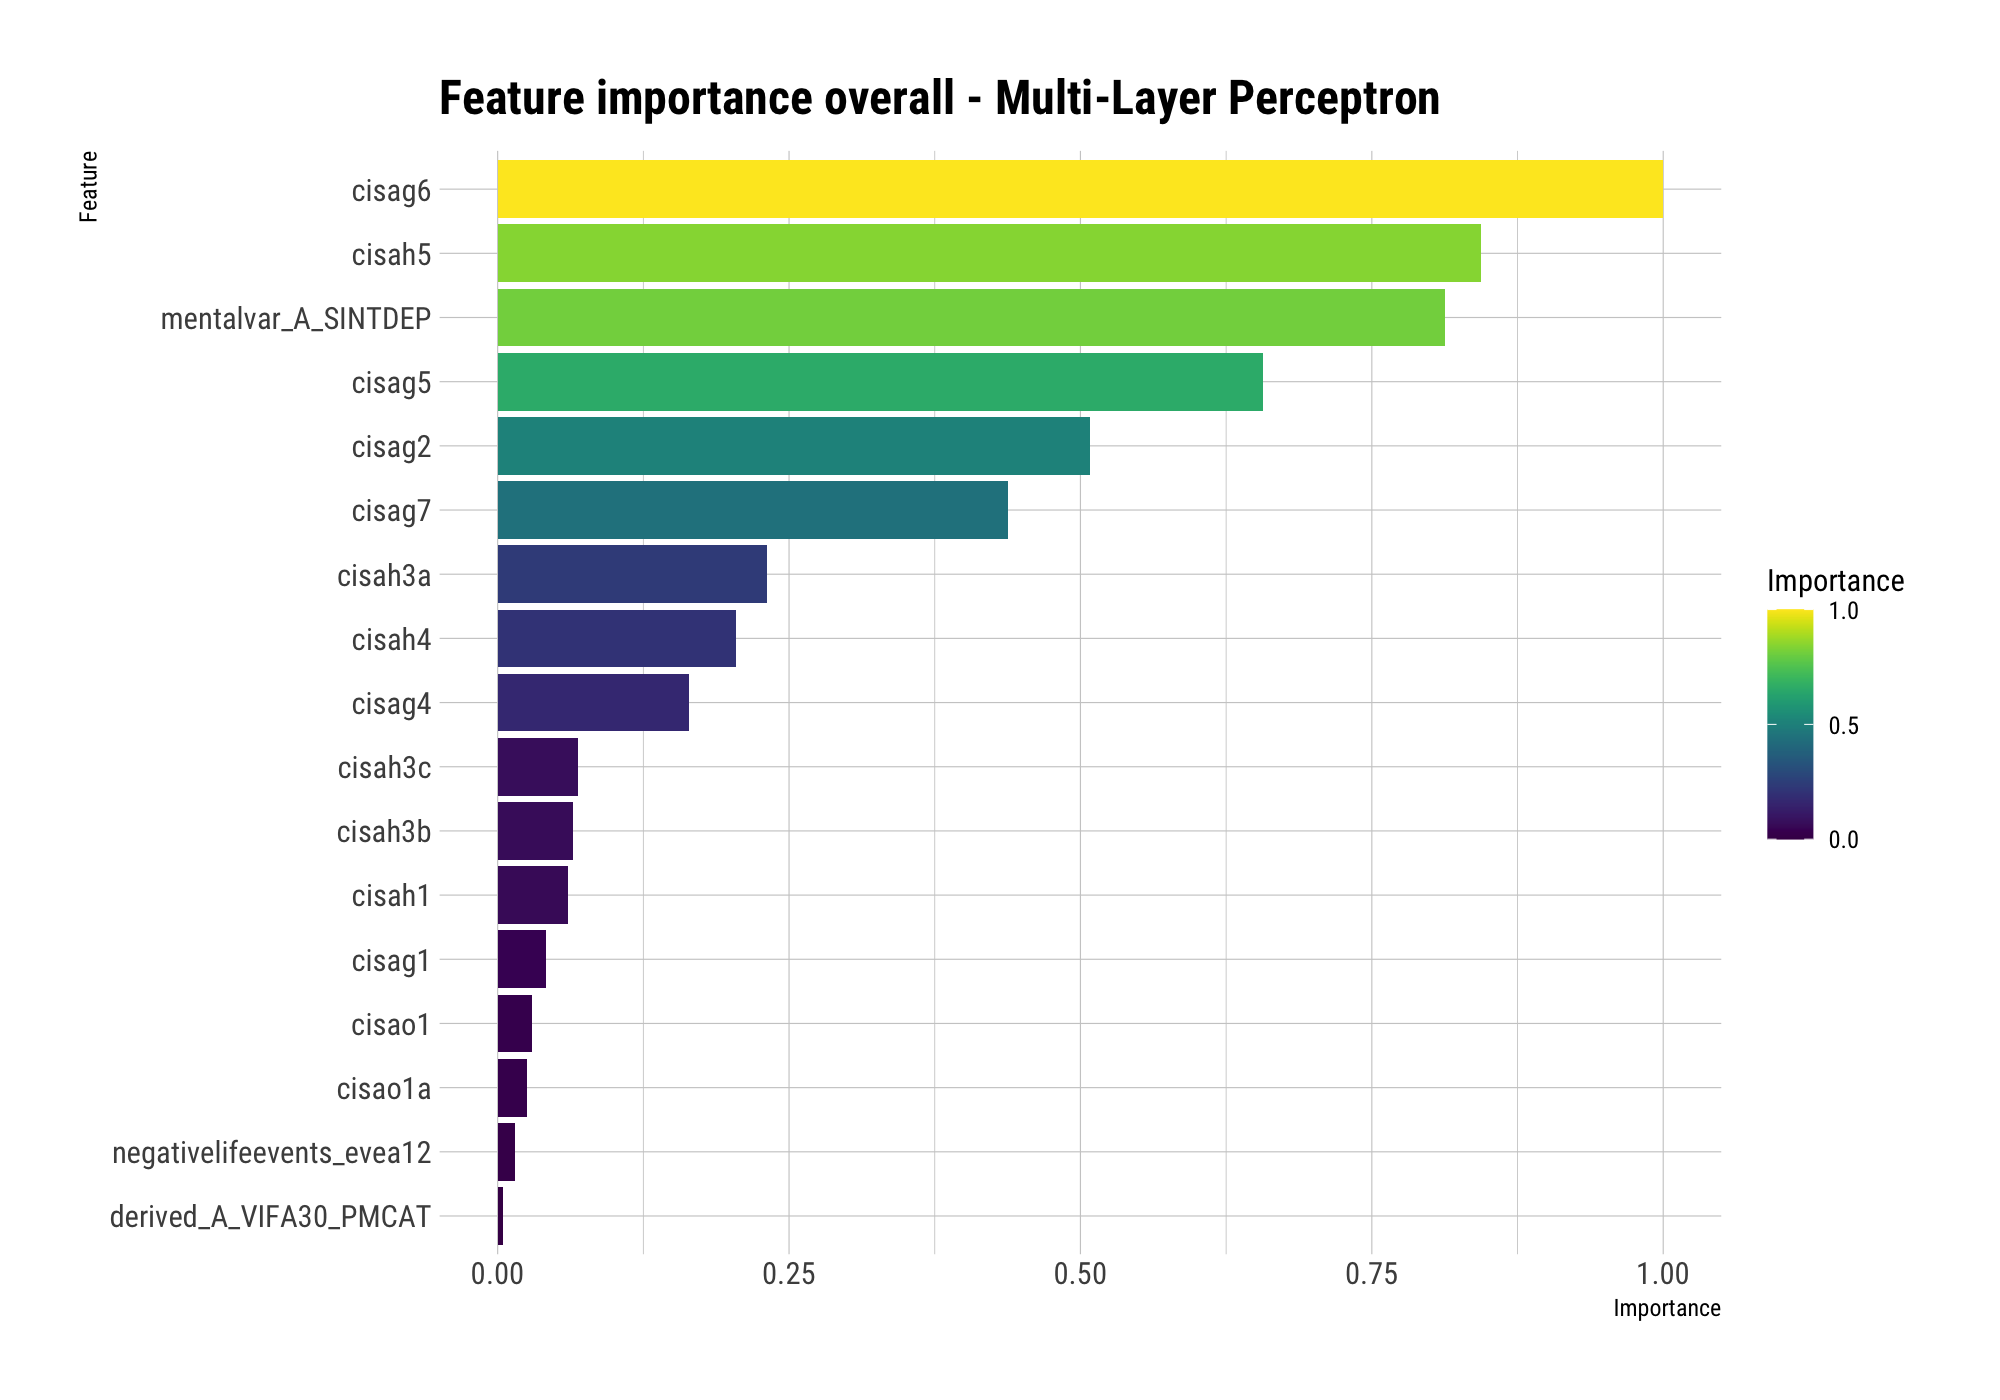
\includegraphics[scale=.21]{../reports/results/models_and_evals/summary/var_imp_mlpML.png}}
    \label{fig:rank-mlp}
\end{figure}

\begin{figure}[H]
    \caption{Rank of attribute relevance for Random Forest}
    \centerline{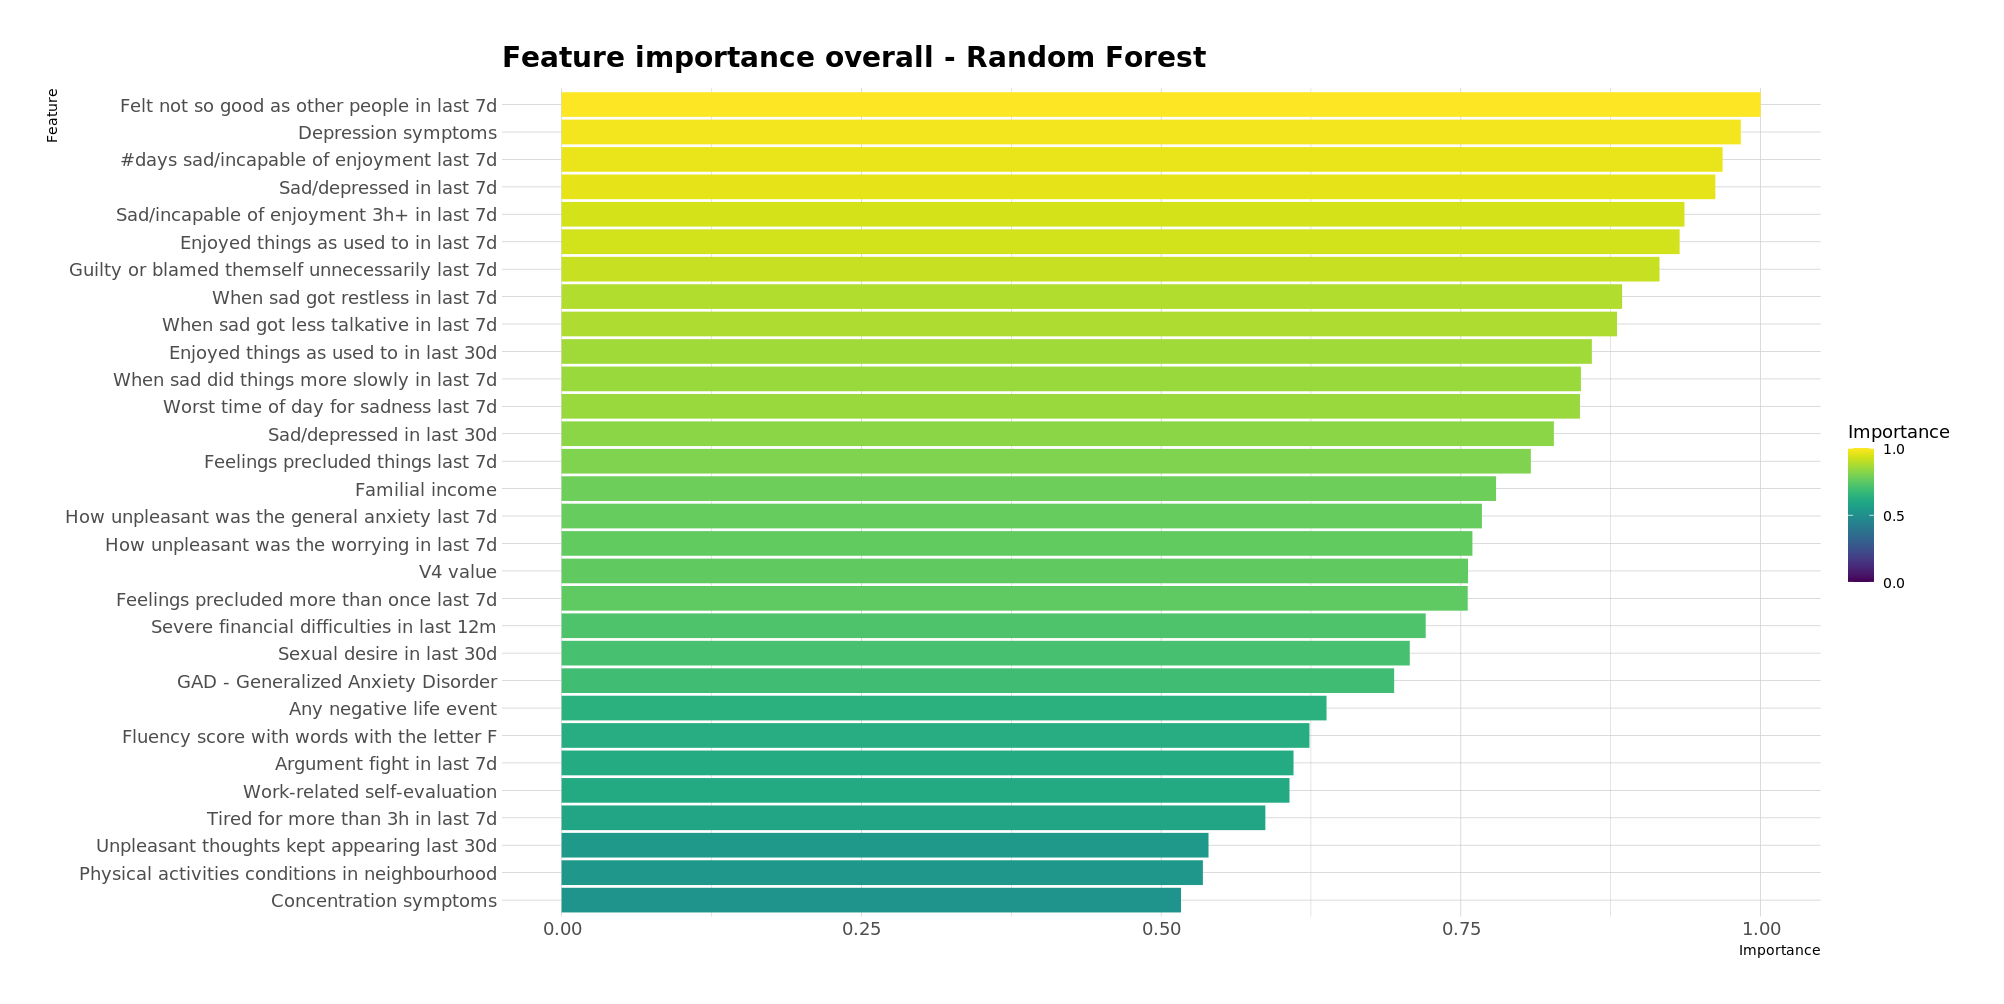
\includegraphics[scale=.21]{../reports/results/models_and_evals/summary/var_imp_ranger.png}}
    \label{fig:rank-ranger}
\end{figure}

\pagebreak

The combination of the three \textit{F\textsubscript{rank}} matrices (which, despite what is shown in Figures~\ref{fig:heatmap-glmnet},~\ref{fig:heatmap-mlp}, ~\ref{fig:heatmap-ranger}, and~\ref{fig:heatmap-ensemble}, includes \textit{all} predictors in the dataset) by averaging the values of the cells in matching positions gives us a form of condensed and summarized knowledge on the criteria used by our classifiers and roughly estimates the attribute importances of our class-probability-averaging ensemble.
We then calculate each predictor's \textit{G\textsubscript{imp}} to sort them by this quantity and again plot the top 30 in a heatmap and in a column chart as was done with the single classifiers.

\begin{figure}[H]
    \caption{Heatmap of attribute relevance for Averaging Ensemble}
    \centerline{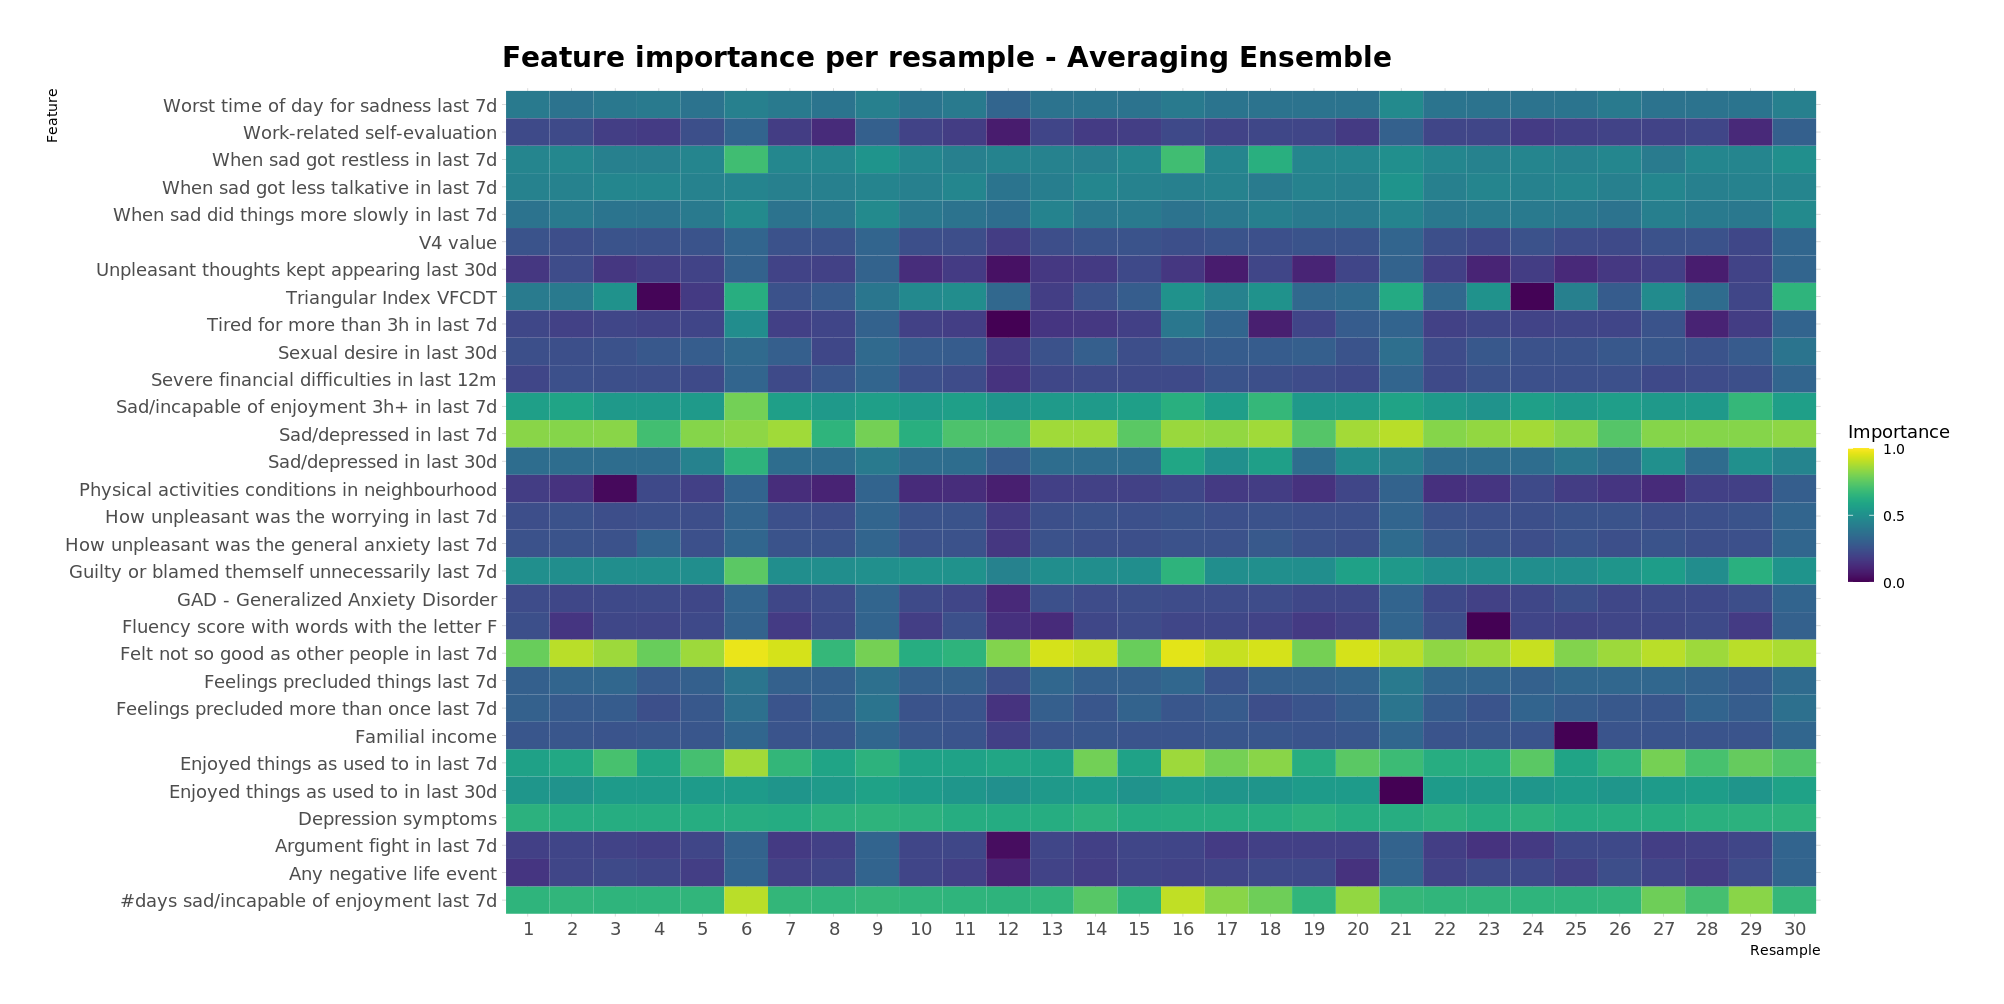
\includegraphics[scale=.22]{../reports/results/models_and_evals/summary/var_imp_resample_aggregation.png}}
    \label{fig:heatmap-ensemble}
\end{figure}

\begin{figure}[H]
    \caption{Rank of attribute relevance for Averaging Ensemble}
    \centerline{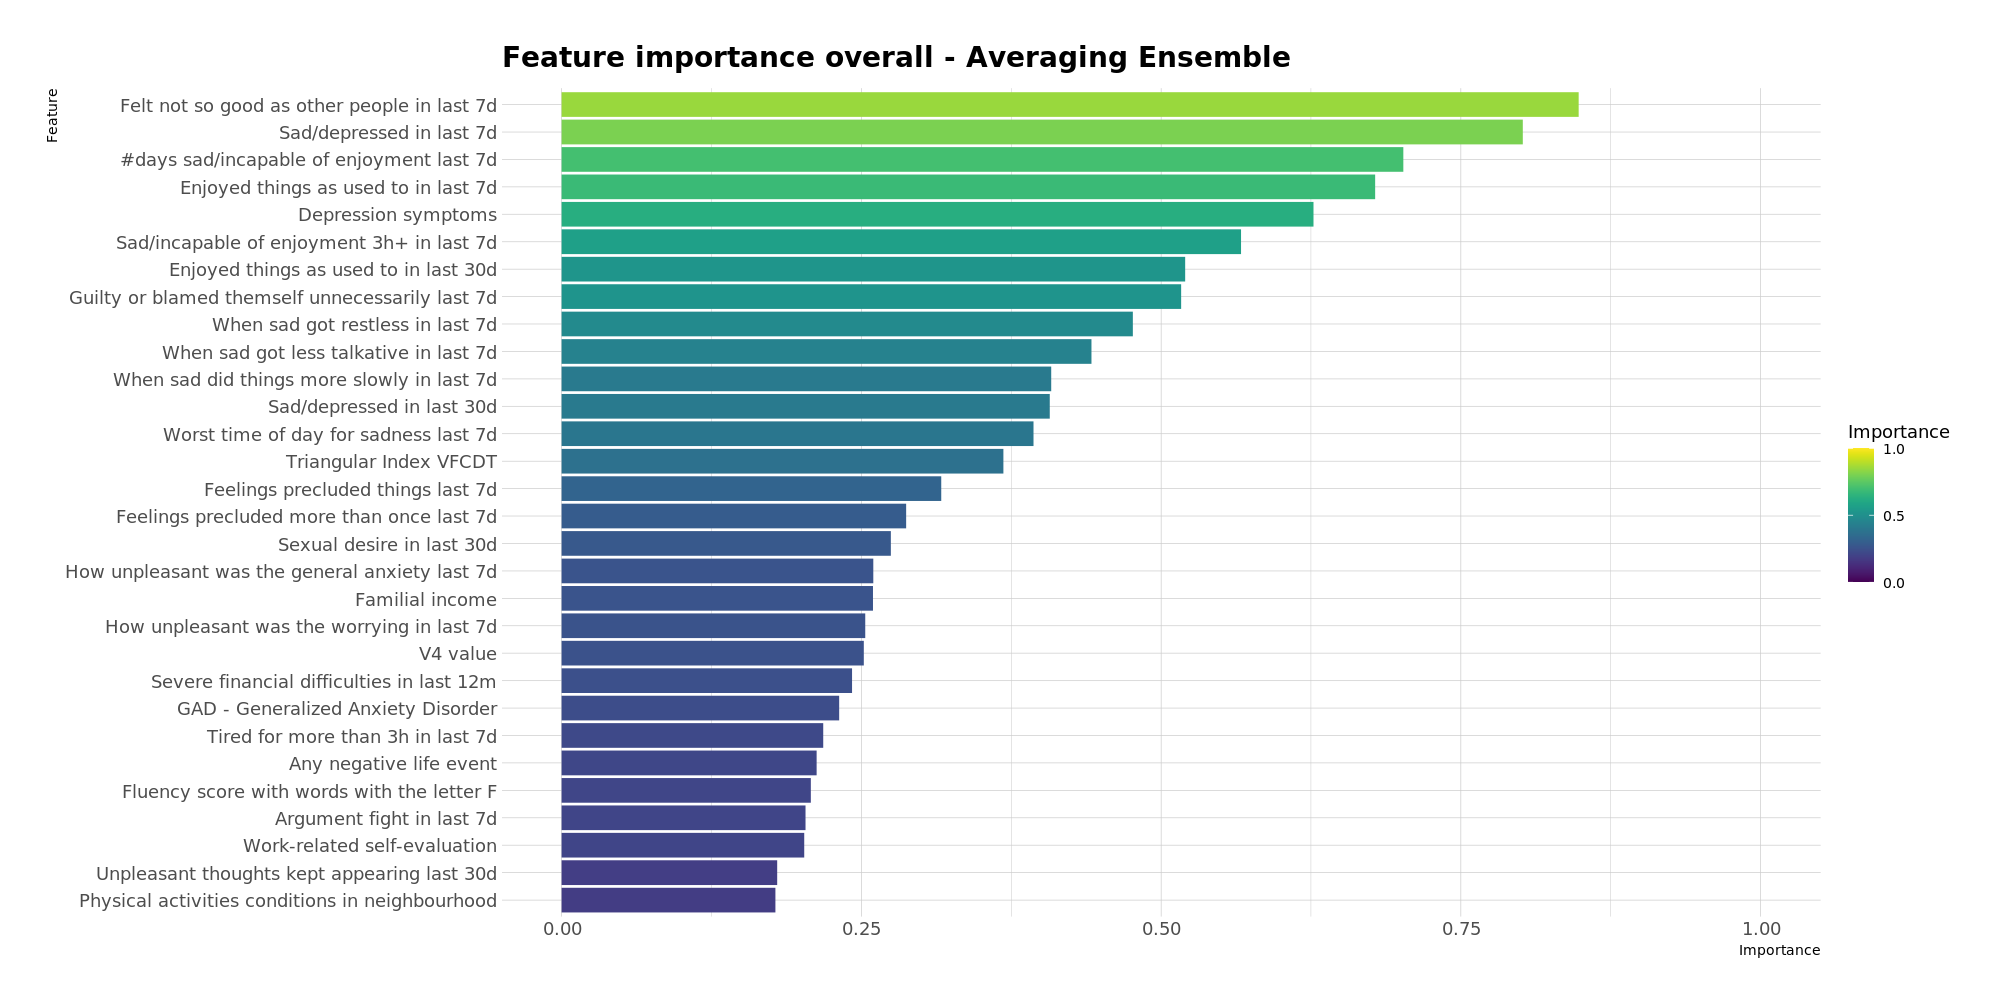
\includegraphics[scale=.21]{../reports/results/models_and_evals/summary/var_imp_aggregation.png}}
    \label{fig:rank-ensemble}
\end{figure}

Regarding the chosen variables per se, Figure~\ref{fig:rank-ensemble} gives us a clear top 5 indicated by the brightest colors and a rather abrupt \textit{G\textsubscript{imp}} jump from the fifth to sixth position, ordered by importance: \textit{cisah5}, \textit{cisag6}, \textit{cisag4}, \textit{cisag5}, and \textit{mentalvar\_A\_SINTDEP}.
All of these are responses to the CIS-R questionnaire, from section G (depression) and H (depressive ideas), safe for \textit{mentalvar\_A\_SINTDEP}, but it relates to the same general theme.
It is worth going over the exact definition of each of the respective questions here, for the analysis and understanding of the models.
Thus, the top-5 variables are, ordered by relevance:

\begin{itemize}
    \item CIS-H5: \textit{During the past week, have you been feeling you are not as good as other people?}
    \item CIS-G6: \textit{Since last (DAY OF WEEK) on how many days have you felt sad, miserable or depressed/unable to enjoy or take an interest in things?}
    \item CIS-G4: \textit{In the past week have you had a spell of feeling sad, miserable, or depressed? Use informant's own words if possible}
    \item CIS-G5: \textit{In the past week have you been able to enjoy or take an interest in things as much as usual? Use informant's own words if possible}
\end{itemize}

\pagebreak

Question H5 stands-out from the others, for its meaning and its calculated \textit{G\textsubscript{imp}} - this indicates our models have an overall consensus that feeling inferior to other people plays a decisive role in increasing the chance of presenting suicidality.
Both G4 and G6 reveal whether the interviewee had been feeling acute sadness, and the G5 and G6 pair provide information on people's loss of interest in things, such that they are not as enjoyable as before.

In short, our models consider as most relevant to their predictions degrees of:
\begin{enumerate}
    \item \textbf{feelings of inferiority} (\textit{cisah5});
    \item \textbf{sadness} (\textit{cisag4, cisag6, cisag7});
    \item \textbf{disappearance of interests} (\textit{cisag2, cisag7});
    \item \textbf{unnecessary guilt} (\textit{cisah4});
    \item \textbf{energy (disposition)} (\textit{cisah3a, cisah3b, cisah3c, cisab5});
    \item \textbf{preclusion} of activities including chores and leisure for bad feelings (\textit{cisao1, cisao1a});
    \item \textbf{income} (\textit{derived\_A\_VIFA30\_PMCAT, negativelifeevents\_evea12});
    \item \textbf{anxiety} (\textit{cisaj8, mentalvar\_A\_TAG});
    \item \textbf{worrying} (\textit{cisai8});
    \item \textbf{libido} (\textit{cisah2});
    \item \textbf{irritability} (\textit{cisae7});
    \item \textbf{obsessions} - or at least recurring bad thoughts (\textit{cisan1});
    \item \textbf{physical activities} (\textit{neighborhood\_viza06)}.
\end{enumerate}

Some outlier variables are found, which cannot be associated with another factor without being too speculative if no further studies on this particular variable are conducted, such as \textit{derived\_cogA\_FLUENCIA\_LETRAF}.
Some predictors relate to physical characteristics and conditions (e.g. \textit{EKG\_a\_vfccl\_triangindex}) in the overall score, but they are found more prominently in the elastic nets' \textit{G\textsubscript{imp}} rank (Figure~\ref{fig:rank-glmnet}), like \textit{derived\_A\_GLOBAL\_RISK} that relate to physical activities, overweight, obesity and metabolic syndrome, and smoking ~\cite{Coke2010}.



    \chapter{Conclusion}\label{ch:conclusions}
    In this chapter, we first reflect on our original goals and the contributions of the current work for the related literature.
Next, we discuss the limitations of the proposed solutions and enhancement opportunities that could be explored in future works.


\section{Contributions and Impact}\label{sec:contributions-and-impact}

\begin{table}[h]
    \caption{Performance estimates of related works compared to ours, ordered by F\textsubscript{2}-Score}
    \begin{center}
        \begin{tabular}{c|c|c|c|c|c}
            \textit{Paper} & \textit{Algorithm} & \textit{F\textsubscript{2}-Score} & \textit{AUCROC} & \textit{Sensitivity} & \textit{Specificity} \\
            \hline
            \hline
            A              & XGB                & \textbf{0.84}                     & 0.86            & 0.79                 & \textbf{0.79}        \\
            B              & ANNs + RF          & 0.71                              & \textbf{0.88}   & 0.80                 & 0.79                 \\
            Ours           & EN + ANN + RF      & 0.69                              & 0.81            & 0.78                 & 0.67                 \\
            C              & ANN                & 0.48                              & 0.88            & \textbf{0.81}        & 0.77                 \\
            D              & EN                 & 0.45                              & 0.79            & 0.67                 & 0.78                 \\
            \hline
        \end{tabular}
    \end{center}
    \legend{Source: The Author

    A: ~\cite{Jung2019};

    B: ~\cite{Roy2020};

    C: ~\cite{Oh2020};

    D: ~\cite{Librenza-Garcia2020}}.
    \label{tab:related-work-vs-ours}
\end{table}

This study proposed and thoroughly tested a solution for identifying patterns of suicidality in a population of Brazilian adults based on data available in the first wave of the ELSA-Brasil study.
Suicidality is defined as the presence of hopelessness, feelings that life is not worth living, and suicidal thoughts.
We made use of special ML techniques chosen based on the challenges and goals of our mission, such that our approach to the problem was focused on minimizing false negative errors (as they are extremely detrimental in our domain) by mitigating the effect of the fewer number of examples labeled as the positive class and yielding high interpretability and insightful knowledge for physicians and clinicians from the produced classifiers.
Thus, although our methodology could be applied to other datasets, our findings in this study elucidate patterns of suicidality in the specific population subset of Brazilian public servants with common mental disorders and do not necessarily directly apply to a more general population.
Nevertheless, we believe the attainment of our goals carries high practical and academic value for dealing with the grave worldwide problem of suicide.

Although direct comparisons to the studies mentioned in Chapter~\ref{ch:related_work} cannot yield fair rankings of performance estimates, given all of them use different datasets (except for~\citet{Librenza-Garcia2020}), it is important to contextualize the findings of this work among the related literature.
That said, in relation to other works with similar objectives but with varying domain particularities, the estimated performance of our models was decently comparable, specially for the F\textsubscript{2}-Score - our optimization metric.
As shown in Table~\ref{tab:related-work-vs-ours}, we achieved very good results in terms of F\textsubscript{2}-Score with our weighted-average ensemble model.
With a mean value of 0.69, our estimated F\textsubscript{2}-Score is close to the second-best work of the table~\cite{Roy2020}.
This promising performance indicator is considerably higher than the ones estimated in~\citet{Oh2020} and~\cite{Librenza-Garcia2020}, with similar data and objectives.

We note that most works do not report the F\textsubscript{2}-Score, and focus on AUCROC, sensitivity, and specificity instead.
The mean area under the ROC curve of our ensemble is, as the other work in the table using the ELSA-Brasil dataset~\cite{Librenza-Garcia2020}, close to 0.8, while other works are closer to the 0.9 mark.
Nonetheless, our results emphasize the importance of using metrics alternative to AUCROC as it does not take precision into account and, thus, can show very satisfactory results even when the models present low true positive rates.
Even though in this work sensitivity and specificity did not achieve results as high as the best ones reported in the related literature, our models presented acceptable scores for these metrics.

Also, our analysis provides important insights about the most relevant features associated with suicidality, which after further investigation by specialists may contribute to new strategies to prevent suicidal ideation and attempts.
Finally, we highlight that during the development of this work we were very careful regarding the methodological and reporting rigor of our research, especially concerning strategies to minimize data leakage and selection biases during model development, which although may result in lower performance provide us with higher confidence regarding the generalization power of our models.


\section{Possible Improvements}\label{sec:possible-improvements}

The first limitation of this work is that it was mainly focused on the computational aspects of the discussed matters, thus it did not examine with all the possible depth the relations between and the explanations of the attributes found to be of most importance to the models.
Also, although we went through what are the most relevant attributes to predict suicidality, since our models are non-linear (safe for the elastic net), we are not able to discuss how variations in each attribute affect the output with the provided analysis material.
Therefore, subsequent studies could analyse how the classification probability varies for each of them, or at least to the most important ones, using for instance Partial Dependence Plots.
With that, stakeholders would have more accurate quantitative insights on the factors related to the class of interest.
Similarly, the understanding of the models could be enriched by an analysis of the commonalities and patterns in the data that cause most classification errors (mainly the false negatives).

Considering the induction of the models to solve our problem, we could also explore different techniques.
Cost-sensitive learning could be implemented and integrated into the procedure, possibly introducing more variation and richness to the constitution of the ensemble, but also a great model by itself.
Other algorithm-level methods to mitigate the class-imbalance problem could be employed, using learners that naturally deal with this such as AdaBoost or eXtreme Gradient Boosting (XGB), or calibrating the probabilities predicted by our model~\cite{Niculescu-Mizil2005}.
These changes would not only provide richness and novelty to the body of literature of the suicidality prediction domain, but also preserve classification robustness in face of a smaller number of positive class instances, allowing future studies to also tackle other ELSA-Brasil dataset variations that are more unbalanced.
For example, studies could consider the whole population instead of only the people presenting CMD, have as outcome label just the suicide ideation variable without combining it with others, or attempt to predict the incidence of suicidality and other labels on ELSA-Brasil's wave 2 based on input data of wave 1.
In terms of data analysed, models could also be built by integrating ELSA-Brasil baseline features georeferenced data, as characteristics related to the geographic location of phenomena may play a role in its occurrence.

Finally, as a more practical application, one could develop user-facing applications to assist clinicians and/or patients and people with common mental disorders.
The programs could use the knowledge uncovered by this study as a basis for a score associated with or some form of journaling done by the user, such that therapists, psychiatrists, and doctors in general can assess their patients' mental health with more tools and have automated support in their decisions.

    \bibliography{biblio}

    \annex


    \chapter{Dataset Variables Descriptions}\label{ch:dataset-variiables-description}
    %\begin{table}[h]
%    \caption{Variables removed during cleansing for having too many absent values}
%    \begin{center}
%        \begin{tabular}{c|c}
%            \textit{Attribute}            & \textit{Description}  \\
%            \hline
%            \hline
%            \textcolor{red}{somevariable} & \textcolor{red}{TODO} \\
%            \hline
%        \end{tabular}
%    \end{center}
%    \legend{Source: The Author}
%    \label{tab:na-removed}
%\end{table}

\begin{table}[h]
    \renewcommand{\arraystretch}{1} % Default value: 1
    \caption{Variables removed during cleansing for being of free-text type}
    \begin{center}
        \begin{tabular}{l|l}
            \textit{Attribute}               & \textit{Description}                      \\
            \hline
            \hline
            anamnesis\_hmpa31h               & Which other join issue (Q31)              \\
            anamnesis\_hmpa37a               & Which cancer (Q37)                        \\
            anamnesis\_hmpa38                & Other health issues (Q38)                 \\
            derived\_A\_CLASSEMEDANTHIPERT   & SAH treatment - drug combinations         \\
            derived\_A\_RCPQOUTROPROBLULT12H & Any health issue last 12h                 \\
            derived\_A\_STATUSVOP            & VOP status                                \\
            dietary\_info\_diea130i          & Reason for diet (Q130)                    \\
            dietary\_info\_diea132p          & What supplement (Q132)                    \\
            dietary\_info\_diea134a          & What coffee (Q134)                        \\
            discrimination\_disa1al          & Work discrimination: reason (Q1a)         \\
            discrimination\_disa2al          & Domestic discrimination: reason (Q2a)     \\
            discrimination\_disa3al          & Police discrimination: reason (Q2a)       \\
            discrimination\_disa4al          & Public discrimination: reason (Q4a)       \\
            discrimination\_disa5al          & School discrimination: reason (Q5a)       \\
            familial\_hfda18d                & Which cancer (father) (Q18)               \\
            familial\_hfda18i                & Which cancer (mother) (Q18)               \\
            familial\_hfda18n                & Which cancer (sibling 1)                  \\
            familial\_hfda18s                & Which cancer (sibling 2)                  \\
            familial\_hfda18y                & Which cancer (sibling 3)                  \\
            home\_info\_vifa03a              & Other conjugal situation (Q4)             \\
            home\_info\_vifa08a              & Partner occupation (Q8)                   \\
            home\_info\_vifa10a              & Who is the other head of family (Q10)     \\
            job\_related\_hoca03             & Main activities in work (Q3)              \\
            job\_related\_hoca14a            & Main activities in work (Q14)             \\
            job\_related\_hoca23a            & Occupation in first job (Q3)              \\
            job\_related\_hoca24a            & Other type of first job (Q4)              \\
            job\_related\_hoca25a            & Who is the other head of family (Q5)      \\
            job\_related\_hoca26             & Other head of family occupation (Q6)      \\
            job\_related\_hoca27a            & Other head of family type of work (Q7)    \\
            job\_related\_hoca32a            & Which other "on duty" scheme (Q12)        \\
            metadata\_centroa                & Investigation center                      \\
            metadata\_ecga3                  & Time (mm:ss)                              \\
            metadata\_rcpadataapini          & CPR date of application                   \\
            negativelifeevents\_evea05a      & Hospitalized 1x: reason (Q5)              \\
            negativelifeevents\_evea07a      & Hospitalized +1x: reasons (Q7)            \\
            others\_cssa11qou                & What other interference in overload       \\
            others\_cssa6                    & Start of ingestion of overload            \\
            others\_cssa7                    & End of ingestion of overload              \\
            others\_esca04                   & End time for interview                    \\
            religion\_hvsa14a                & What other religion (Q14)                 \\
            socio\_economic\_psea05a         & Color or race (Q5)                        \\
            socio\_economic\_psea08a         & What other condition of the property (Q8) \\
            women\_mula17m                   & What other contraceptive (Q17)            \\
            women\_mula20b                   & Missing medical data                      \\
            women\_mula22h                   & \textit{<No description>}                 \\
            women\_mula30b                   & Missing medical data hormonal             \\
            women\_mula5g                    & What reasons stopped menstruating (Q5)    \\
            \hline
        \end{tabular}
    \end{center}
    \label{tab:free-text-removed}
\end{table}

%\begin{table}[h]
%    \caption{All variables made available from the ELSA-Brasil dataset, after cleansing}
%    \begin{center}
%        \begin{tabular}{c|c}
%            \textit{Attribute}            & \textit{Description}  \\
%            \hline
%            \hline
%            \textcolor{red}{somevariable} & \textcolor{red}{TODO} \\
%            \hline
%        \end{tabular}
%    \end{center}
%    \legend{Source: The Author}
%    \label{tab:elsa-dataset-all-variables}
%\end{table}


    \chapter{CIS-R Questionnaire}\label{ch:cis-r}
    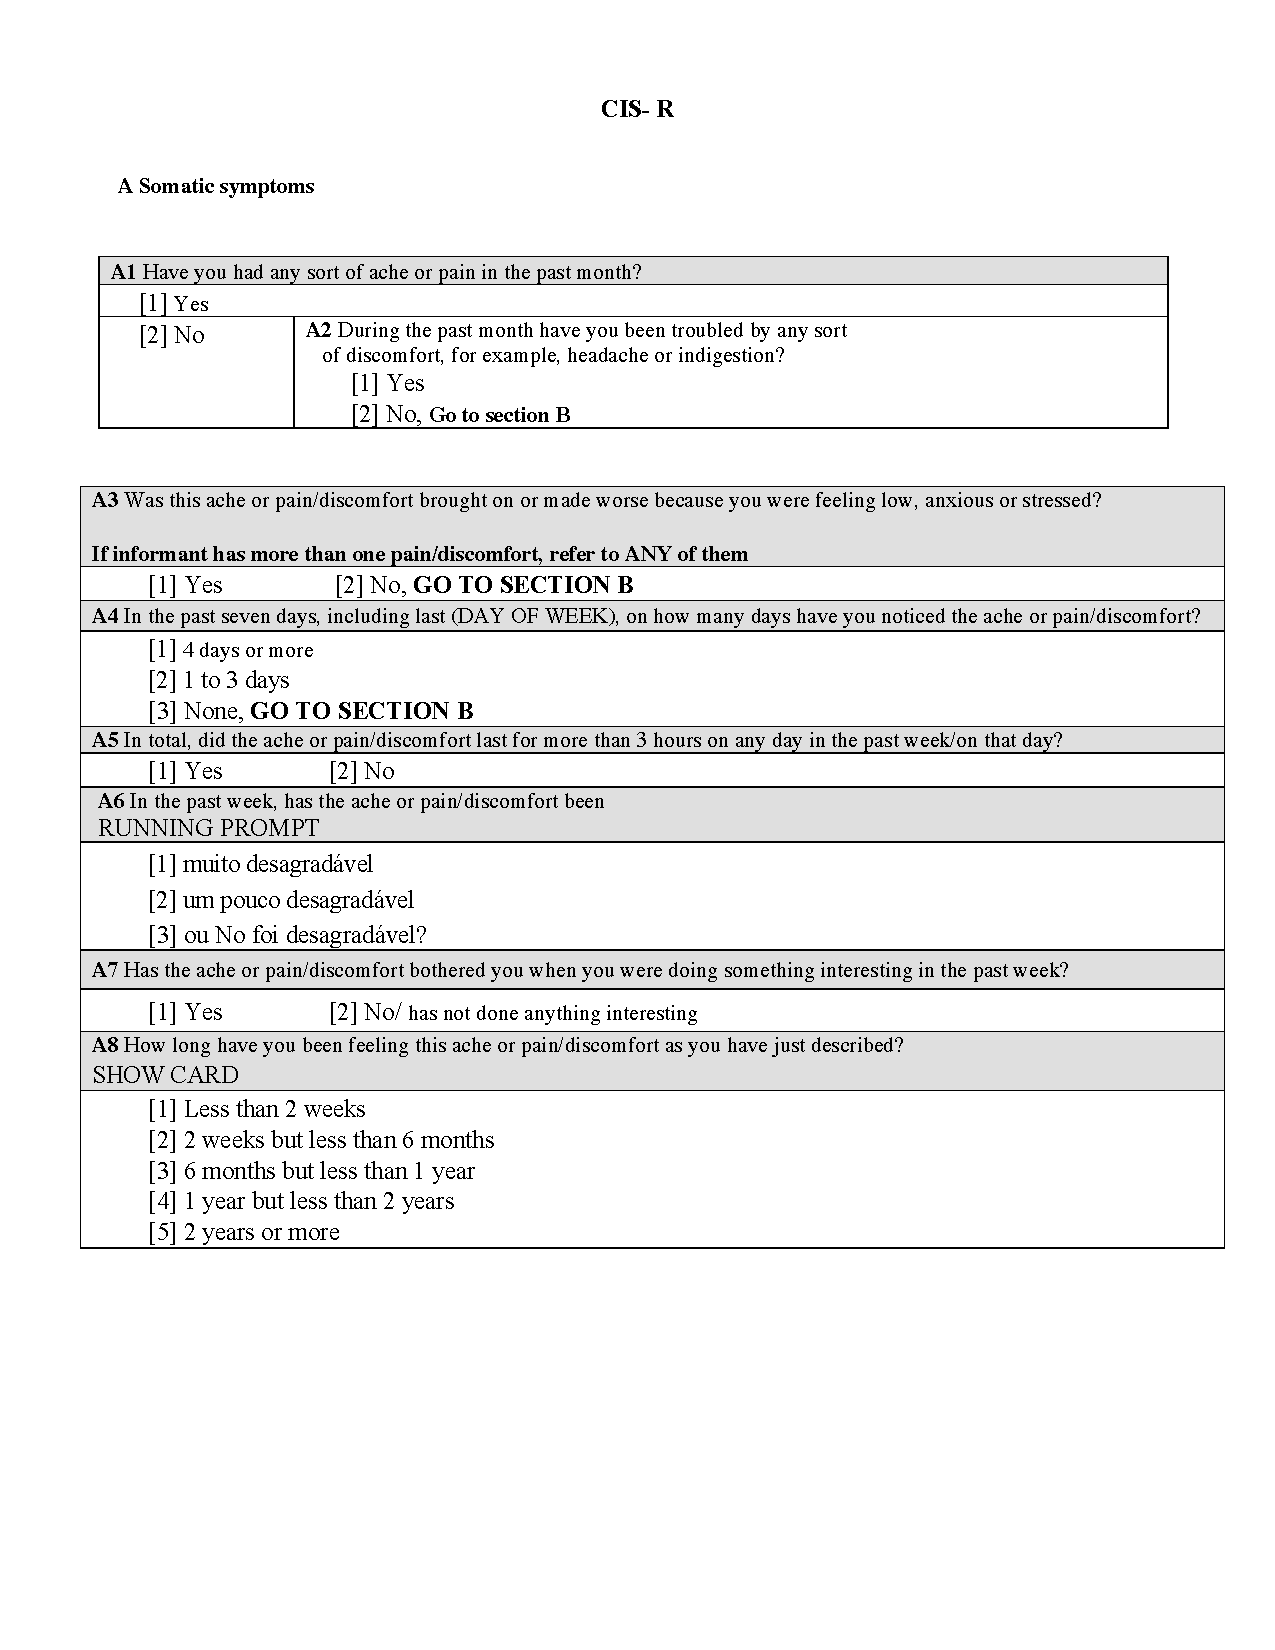
\includepdf[pages=-]{cis-r.pdf}

\end{document}
